%\usepackage[utf8]{inputenc}
%\usepackage[round,authoryear]{natbib}


\documentclass[11pt]{article}
\usepackage[margin=1in]{geometry}
\usepackage{url,hyperref}
\usepackage{graphicx}
\usepackage{amsmath,amssymb,array,eucal, amsthm}
\linespread{1.45}
\setlength\parindent{35pt}
\DeclareMathOperator{\sgn}{sgn}
\newcommand{\e}{\mathbf{e}}
\renewcommand{\P}{\mathbf{P}}
\newcommand{\F}{\mathbf{F}}
\newcommand{\mat}[1] {\mathbf{#1}}
%\newcommand{\ind}{\mathrel{\mathop{\sim}\limits^{\mathit{ind}}}}
%\newcommand{\iid}{\mathrel{\mathop{\sim}\limits^{\mathit{iid}}}}
\newcommand{\SE}{\textsf{SE}}
\newcommand{\SSE}{\textsf{SSE}}
\newcommand{\RSS}{\textsf{RSS}}
\newcommand{\FSS}{\textsf{FSS}}
\renewcommand{\SS}{\textsf{SS}}
\newcommand{\MSE}{\textsf{MSE}}
\newcommand{\SSR}{\textsf{SSR}}
\newcommand{\Be}{\textsf{Beta}}
\newcommand{\St}{\textsf{St}}
\newcommand{\Ca}{\textsf{C}}
\newcommand{\Exp}{\textsf{Exp}}
\newcommand{\TruncExp}{\textsf{TruncExp}}
\newcommand{\TruncWeibull}{\textsf{TruncWeibull}}
\newcommand{\GDP}{\textsf{GDP}}
\newcommand{\NcSt}{\textsf{NcSt}}
\newcommand{\Bin}{\textsf{Bin}}
\newcommand{\NB}{\textsf{NegBin}}
\renewcommand{\NG}{\textsf{NG}}
\newcommand{\No}{\textsf{N}}
\newcommand{\Ber}{\textsf{Ber}}
\newcommand{\Poi}{\text{Poi}}
\newcommand{\Gam}{\textsf{Gamma}}
\newcommand{\BB}{\textsf{BB}}
\newcommand{\Gm}{\textsf{G}}
\newcommand{\Un}{\textsf{Unif}}
\newcommand{\Ex}{\textsf{Exp}}
\newcommand{\DE}{\textsf{DE}}
\newcommand{\tr}{\textsf{tr}}
\newcommand{\cF}{{\cal{F}}}
\newcommand{\cL}{{\cal{L}}}
\newcommand{\cI}{{\cal{I}}}
\newcommand{\cB}{{\cal{B}}}
\newcommand{\cP}{{\cal{P}}}
\newcommand{\bbR}{\mathbb{R}}
\newcommand{\bbN}{\mathbb{N}}
\newcommand{\pperp}{\mathrel{{\rlap{$\,\perp$}\perp\,\,}}}
\newcommand{\OFP}{(\Omega,\cF, \P)}
\newcommand{\eps}{\boldsymbol{\epsilon}}
\newcommand{\1}{\mathbf{1}_n}
\newcommand{\gap}{\vspace{8mm}}
\newcommand{\ind}{\mathrel{\mathop{\sim}\limits^{\rm ind}}}
\newcommand{\simiid}{\ensuremath{\mathrel{\mathop{\sim}\limits^{\rm
iid}}}}
\newcommand{\eqindis}{\ensuremath{\mathrel{\mathop{=}\limits^{\rm D}}}}
\newcommand{\iid}{\textit{i.i.d.}}
\newcommand{\SSZ}{S_{zz}}
\newcommand{\SZW}{S_{zw}}
\newcommand{\Var}{\textsf{Var}}
\newcommand{\corr}{\textsf{corr}}
\newcommand{\diag}{\textsf{diag}}
\newcommand{\var}{\textsf{var}}
\newcommand{\Cov}{\textsf{Cov}}
\newcommand{\Sam}{{\cal S}}
\def\H{\mathbf{H}}
\newcommand{\Y}{\mathbf{Y}}
\newcommand{\tY}{\tilde{\mathbf{Y}}}
\newcommand{\Yhat}{\hat{\mathbf{Y}}}
\newcommand{\Yobs}{\mathbf{Y}_{{\cal S}}}
\newcommand{\barYobs}{\bar{Y}_{{\cal S}}}
\newcommand{\barYmiss}{\bar{Y}_{{\cal S}^c}}

\newcommand{\iton}{i=1,\dots,n}
\newcommand{\itom}{i=1,\dots,m}
\newcommand{\ktoK}{k=1,\dots,K}

\def\bv{\mathbf{b}}
\def\av{\mathbf{a}}
\def\X{\mathbf{X}}
\def\tX{\tilde{\mathbf{X}}}
\def\x{\mathbf{x}}
\def\xbar{\bar{\mathbf{x}}}
\def\Xbar{\bar{\mathbf{X}}}
\def\Xg{\mathbf{X}_{\boldsymbol{\gamma}}}
\def\Ybar{\bar{\Y}}
\def\ybar{\bar{y}}
\def\y{\mathbf{y}}
\def\Yf{\mathbf{Y_f}}
\def\W{\mathbf{W}}
\def\L{\mathbf{L}}
\def\w{\mathbf{w}}
\def\U{\mathbf{U}}
\def\V{\mathbf{V}}
\def\Q{\mathbf{Q}}
\def\Z{\mathbf{Z}}
\def\z{\mathbf{z}}
\def\v{\mathbf{v}}
\def\u{\mathbf{u}}


\def\R{\mathbb{R}}
\def\N{\mathbb{N}}
\def\E{\mathscr{E}}
\def\I{\mathscr{I}}
\def\s{\sigma}
\def\ra{\rightarrow}

\def\zero{\mathbf{0}}
\def\one{\mathbf{1}}

\def\EE{(E, \E)}

\newcommand{\taub}{\boldsymbol{\tau}}
\newcommand{\betav}{\boldsymbol{\beta}}
\newcommand{\alphav}{\boldsymbol{\alpha}}
\newcommand{\A}{\mathbf{A}}
\def\a{\mathbf{a}}
\def\K{\mathbf{K}}
\newcommand{\B}{\mathbf{B}}
\def\b{\boldsymbol{\beta}}
\def\bhat{\hat{\boldsymbol{\beta}}}
\def\btilde{\tilde{\boldsymbol{\beta}}}
\def\tb{\boldsymbol{\theta}}
\def\bg{\boldsymbol{\beta_\gamma}}
\def\bgnot{\boldsymbol{\beta_{(-\gamma)}}}
\def\mub{\boldsymbol{\mu}}
\def\tmub{\tilde{\boldsymbol{\mu}}}
\def\muhat{\hat{\boldsymbol{\mu}}}
\def\tb{\boldsymbol{\theta}}
\def\tk{\boldsymbol{\theta}_k}
\def\tj{\boldsymbol{\theta}_j}
\def\Mk{\boldsymbol{{\cal M}}_k}
\def\M{\boldsymbol{{\cal M}}}
\def\Mj{\boldsymbol{{\cal M}}_j}
\def\Mi{\boldsymbol{{\cal M}}_i}
\def\Mg{{\boldsymbol{{\cal M}_\gamma}}}
\def\Mnull{\boldsymbol{{\cal M}}_{N}}
\def\gMPM{\boldsymbol{\gamma}_{\text{MPM}}}
\def\gHPM{\boldsymbol{\gamma}_{\text{HPM}}}
\def\Mfull{\boldsymbol{{\cal M}}_{F}}
\def\tg{\boldsymbol{\theta}_{\boldsymbol{\gamma}}}
\def\g{\boldsymbol{\gamma}}
\def\eg{\boldsymbol{\eta}_{\boldsymbol{\gamma}}}
\def\G{\mathbf{G}}
\def\cM{\cal M}
\def\D{\Delta}
\def \shat{{\hat{\sigma}}^2}
\def\uv{\mathbf{u}}
\def\l {\lambda}
\def\d{\delta}
\def\Sigmab{\boldsymbol{\Sigma}}
\def\Lambdab{\boldsymbol{\Lambda}}
\def\lambdab{\boldsymbol{\lambda}}
\def\Mg{{\cal M}_\gamma}
\def\S{{\cal{S}}}
\def\qg{p_{\boldsymbol{\gamma}}}
\def\pg{p_{\boldsymbol{\gamma}}}
%\def\t{\mathbf{t}}
\def\T{\boldsymbol{\Theta}}
\def\Tb{\boldsymbol{\Theta}}

\usepackage{algorithm}
\usepackage{algorithmic}
\usepackage{caption}
\usepackage{subcaption}
\usepackage{color}


\graphicspath{ {../Figures/} }

\newcommand{\jx}[1]{{\color{blue}{ #1}}}
\newcommand{\ram}[1]{{\color{green}{ #1}}}
\newcolumntype{C}[1]{>{\centering\let\newline\\\arraybackslash\hspace{0pt}}m{#1}}

\newtheorem{theorem}{Theorem}[section]
\newtheorem{proposition}{Proposition}[section]
\newtheorem{lemma}{Lemma}[section]

\begin{document}
	
	% Keywords command
	\providecommand{\keywords}[1]
	{
		\small	
		\textbf{\textit{Keywords---}} #1
	}
	
	
	\title{%Efficient Likelihood-Based Inference for Fitting Stochastic Epidemic Models to Incidence Data via Data Augmentation
		Uniformly Ergodic Data-Augmented MCMC for Fitting the General Stochastic Epidemic Model to Incidence Data}
		
	\author{
	Rapha\"{e}l Morsomme$^{1}$\footnote{raphael.morsomme@duke.edu} \ and Jason Xu$^{1}$ \\
	\small $^{1}$Department of Statistical Science, Duke University \\
	}
	\date{
	\today
	}	
	\maketitle
	
	\begin{abstract}
		Stochastic epidemic models provide an interpretable probabilistic description of the spread of a disease through a population. Yet, fitting these models when the epidemic process is only partially observed is a notoriously difficult task due to the intractability of the likelihood for many classical models. To remedy this issue, this article introduces a novel data-augmented MCMC algorithm for fast and exact inference for the stochastic SIR model given discretely observed incidence counts of infection. In a Metropolis-Hastings step, the algorithm jointly proposes the augmented data from a surrogate stochastic process whose dynamics closely resemble those of the SIR process, and from which we can efficiently generate an epidemic that is compatible with the observed data. Not only is the algorithm fast, but since the augmented data are generated from a faithful approximation of the target model, the method can update large portions of the latent space per iteration without prohibitively lowering the acceptance rate. We find that the method explores the high-dimensional latent space efficiently and show that the Markov chain underlying the algorithm is uniformly ergodic.
		The proposed algorithm enables exact Bayesian inference that scales to outbreaks with hundreds of thousands of individuals,  even on a single laptop. We validate its performance via thorough simulation experiments and a case study on the 2013-2015 Ebola outbreak in Western Africa.
	\end{abstract}
	\keywords{Stochastic SIR model; incidence data; exact Bayesian inference; data-augmented MCMC; likelihood-based methods; uniform ergodicity}
	
	\section{Introduction}
	% Outline: SEM; intractable likelihood; existing methods: approximation (Cauchemez 2008, Fintzi 2020), particle filtering, ABC, data augmentation; poor mixing; 
	
	The efficient control of a disease outbreak requires an understanding of the mechanisms underlying its spread. Mechanistic compartmental models, which describe the transition of individuals between various states, have a long mathematical modeling tradition in epidemiology \cite{Kermack.1927}. Due to their interpretability, they are commonly used to describe the dynamics of an outbreak and typically serve as the main source of information for predicting the course of an outbreak and identifying interventions that could be effective. Originally, deterministic versions of the models were employed by mathematicians and epidemiologists. These models are simple to analyze, but fail to capture the inherent randomness characterizing the spread of a disease. For instance, they cannot be used to estimate the probability of a large-scale outbreak or its expected duration, and do not allow for uncertainty quantification when used within inferential procedures. Stochastic epidemic models (SEM), on the other hand, incorporate the random nature of infections and recoveries and therefore provide more realistic descriptions of the spread of a disease, and in turn more reliable inference from observed data.
	
	Conducting inference on SEMs is, however, a notably difficult task. Challenges stem from the fact that the observed data typically provide incomplete information on a process that evolves continuously through time, making the likelihood of the model intractable. %Were the infection and recovery times of each individual of the population observed, inference would be straightforward, but this is rarely the case. 
	In practice, one often has access to either incidence data such as weekly counts of new infections, or prevalence data such as the numbers of infectious individuals at discrete reporting times. The marginal likelihood of such partially observed data becomes a computational bottleneck, as it requires a large integration step that accounts for all possible configurations of the missing epidemic process. In particular, direct computation of this likelihood requires the transition probabilities between observation times for which no closed form is available. Moreover, given the size of the transition matrix, classical matrix exponentiation is intractable. %\jx{to do: cite recent papers from Simon Spencer's group too that do so for discrete-time models, and mention classical matrix exponentiation being intractable}.
	Numerical methods to obtain transition probabilities have only recently been developed in \cite{Ho.2018b, Ho.2018}, but the high computational costs limit their approach to moderate sized outbreaks.
	
	In this article, we employ data augmentation to explore configurations of the missing data through latent variables. We introduce a uniformly ergodic data-augmented MCMC (DA-MCMC) algorithm that targets the exact joint posterior of model parameters and these latent variables under the stochastic SIR model, a commonly used SEM, from discretely observed incidence counts of infections. Rather than marginalizing directly, our approach accounts for the latent space via sampling. The algorithm updates the event times of the augmented data by jointly proposing infection and removal times from a surrogate stochastic process whose dynamics closely resemble those of the SIR process, and from which we can efficiently generate an epidemic that is compatible with the observed data. Its success lies in the design of this surrogate process serving as an efficient proposal scheme within a Metropolis-Hastings algorithm. Since the latent spaces are generated from a faithful approximation of the target epidemic model, the algorithm can update a large portion of the event times per iteration while maintaining a high acceptance rate, thereby exploring the high-dimensional latent space efficiently. Our approach is fully Bayesian and therefore allows representation of parameter uncertainty through posterior distributions.
	
	The remainder of the article is structured as follows. Section \eqref{sec:set} provides background information on the inference task. It introduces the stochastic SIR model and explains why conducting inference from partially observed data is a difficult task. Previous works addressing this problem are also presented. Section \eqref{sec:pds} introduces the DA-MCMC algorithm and describes the surrogate process from which the latent data are generated in the Metropolis-Hastings step. The similarity between the surrogate and the target processes is assessed in Section \eqref{sec:qua} and the DA-MCMC is shown to be uniformly ergodic in Section \eqref{sec:uni}. In Section \eqref{sec:sim}, we examine the performance of our algorithm on simulated data and then turn to an analysis of the 2013-2015 Ebola outbreak in Gu\'eck\'edou, Guinea, in Section \eqref{sec:ebo}. Finally, Section \eqref{sec:dis} discusses the findings and concludes the article.
	
	\section{Background and Prior Work}
	\label{sec:set}
	%Outline: compartmental model; CTMC; rates; likelihood; inference (MLE, gamma conjugacy)
	
	\subsection{The Stochastic SIR Model}
	\label{sec:sir}
	%Outline: stochastic SIR; X; parameters; transition rate12
	
	Our point of departure is to consider the stochastic SIR model -- also referred to as the general stochastic epidemic model \cite{Bailey.1975} -- which offers a parsimonious and interpretable representation of the mechanistic dynamics of an epidemic. The stochastic SIR model is a compartmental model in which individuals transition through three states or compartments: susceptible (S), infectious (I) and removed (R). The only possible moves are from S to I (infections) and from I to R (removals). A susceptible individual becomes infected through contact with an infectious individual. Once infected, she is immediately infectious and remains so for some period of time after which she is removed from the process without the possibility of reinfection. In this formulation, demographic dynamics such as births and deaths are ignored since they usually occur at a much slower rate than infections and removals.
	
	Assuming a closed population of size $n$, the stochastic SIR model consists of a continuous-time vector-valued process
	\begin{equation}
		\label{eq:X}
		\X = \left\lbrace \X(t), t>0\right\rbrace \in \chi_{\X}
	\end{equation}
	with
	\begin{equation}
		\X(t) = \left(X_1(t), \dots, X_n(t)\right) \in \{s, i, r\}^n
	\end{equation}
	where the agent-level subprocess
	$$ X_j(t) = 
	\begin{cases}
		s, & t \in [0, \tau^I_j] \\
		i, & t \in (\tau^I_j, \tau^R_j] \\
		r, & t \in (\tau^R_j, \infty)
	\end{cases}
	,\quad \iton
	$$
	denotes the compartment of individual $j$ at time $t$ with $\tau^I_j$ and $\tau^R_j$ respectively the infection and removal times of individual $j$. If individual $j$ never becomes infectious, we set $\tau^I_j = \tau^R_j = \infty$ and $X_j(t) = s$ for $t \in [0, \infty)$. Since removed individuals do not contribute to the pandemic, it is safe to ignore the individuals removed at time $0$ and write $n = S(0) + I(0)$. Here the space $\chi_{\X}$ denotes the set of trajectories compatible with the evolution of a disease---that is, the set of trajectories in which no infection occurs when the infectious compartment is depleted:
	\begin{equation}
		\label{eq:chi}
		\chi_{\X} = \{\X:\X(t) \in \{s,r\}^n \Rightarrow \X(t+u) = \X(t), \forall u>0 \}.
	\end{equation}
	
	The stochastic SIR model is specified by the rates at which individuals move from one compartment to another. If we assume a homogeneously mixing population where contacts between individuals occur independently at some constant rate $\beta$, the contacts between two given individuals are said to follow a Poisson process with rate $\beta$. This parameter can be interpreted as the \textit{infection rate}: when a susceptible individual comes into contact with an infectious individual, she immediately becomes infectious.
	If we also make the common assumption that the infectious periods follow independent exponential distributions with rate $\gamma$, then the process \eqref{eq:X} is a time–homogeneous continuous time Markov chain, whose instantaneous transition rates
	are given by the matrix $\Lambda = [\lambda_{\x, \x'}]$ with
	\begin{equation}
	\label{eq:rate}
    	\lambda_{\x, \x'} = 
    	\begin{cases}
    		\beta I(t), & \x \text{ and } \x' \text{ only differ at position } j \text{ with } x_j = s \text{ and } x_j' = i, \\
    		\gamma, & \x \text{ and } \x' \text{ only differ at position } j \text{ with } x_j = i \text{ and } x_j' = r, \\
    		0, & \text{ otherwise.}
    	\end{cases}
	\end{equation}
	where $I(t) = \#\{x_j(t) = i\}$ is the total number of infectious individuals at time $t$. Thus, the individual-level infection and removal rates at time $t$ are respectively $\beta I(t)$ and $\gamma$.

	%Equivalently \jx{The following is not an exact equality, but needs the $o(dt)$ term or similar}
	%	$$
	%	P(\X_t = \x, \X_{t+dt} = \x') =
	%	\begin{cases}
	%		\beta I(t) dt + o(dt), & \x \text{ and } \x' \text{ only differ at position } j \text{ with } x_j = S \text{ and } x_j' = I, \\
	%		\gamma dt + o(dt), & \x \text{ and } \x' \text{ only differ at position } j \text{ with } x_j = I \text{ and } x_j' = R, \\
	%		o(dt), & \text{otherwise}
	%	\end{cases}
	%	$$
	%	where $dt>0$ is small.
	
	
	\subsection{Inference with Complete Data}
	\label{sec:icd}
	%Outline: complete-data likelihood; MLE; gamma conjugacy
	
	When the Markov process \eqref{eq:X} is completely observed until time $t_{end}$, we obtain the following likelihood \cite{Streftaris.2002}
	\begin{align}
		L(\theta; \X)
		& = \prod_{j \in \mathcal{I}} \beta I(\tau^I_j) \prod_{k \in \mathcal{R}} \gamma \exp\left\lbrace - \int_{0}^{t_{end}}\beta S(t)I(t) + \gamma I(t) dt \right\rbrace  \nonumber \\
		\label{eq:cdl}
		& = \beta^{n_I} \gamma^{n_R}\prod_{j \in \mathcal{I}} I(\tau^I_j) \exp\left\lbrace - \beta \int_{0}^{t_{end}} S(t)I(t) - \gamma \int_{0}^{t_{end}} I(t) dt \right\rbrace
	\end{align}
	describing the complete data trajectory.
	To establish notation,
	$\theta = (\beta, \gamma) \in \chi_{\theta}$ are the model parameters 
	and $\chi_{\theta} = (0, \infty) \times (0, \infty)$ denotes the parameter space, 
	the index sets $\mathcal{I} = \{j: \tau^I_j \in (0, t_{end}]\}$ and $\mathcal{R} = \{j: \tau^R_j \in (0, t_{end}]\}$ denote the individuals that are respectively infected and removed during the observation interval $(0, t_{end}]$,
	$n_I = |\mathcal{I}|$ and $n_R = |\mathcal{R}|$ are the numbers of observed infections and removals,
	and	$S(t) = \#\{X_i(t) = s\}$ is the number of susceptible individuals at time $t$.
	
	It is straightforward to conduct inference in this continuously observed scenario \cite{Guttorp.2018}. The likelihood \eqref{eq:cdl} belongs to the exponential family, and maximum likelihood estimates of its parameters can be expressed in terms of the sufficient statistics defined above as 
	$$
	\hat{\beta} = \dfrac{n_I}{ \int_{0}^{t_{end}} S(t)I(t)dt}, \qquad \hat{\gamma} = \dfrac{n_R}{ \int_{0}^{t_{end}} I(t)dt}.
	$$
	Note that since the functions $I(t)$ and $S(t)$ are constant between event times, the two integrals correspond to finite sums which are straightforward to compute.
	Furthermore, in a Bayesian context, inference is facilitated by the conjugacy of \eqref{eq:cdl} with the gamma distribution. If we use independent gamma priors
	\begin{equation}
		\label{eq:pri}
		\beta \sim G(a_{\beta}, b_{\beta}), \qquad \gamma \sim G(a_{\gamma}, b_{\gamma})
	\end{equation}
	where $G(a,b)$ denotes the parametrization of the gamma distribution with mean $a/b$ and variance $a/b^2$, we obtain the independent posterior distributions
	\begin{align}
		\label{eq:posterior_theta}
		\beta | \X & \sim G\left( a_{\beta} + n_I , b_{\beta} + \int_{0}^{t_{end}} I(t)S(t) dt\right) \\
		\gamma | \X & \sim G\left( a_{\gamma} + n_R, b_{\gamma} + \int_{0}^{t_{end}} I(t) dt\right)
	\end{align}
	from which one can easily generate independent values to explore the distribution $\pi(\theta|\X)$ via Monte Carlo.
	
	The likelihood \eqref{eq:cdl} can also be parameterized in terms of $\tilde{\theta} = (\beta, R_0)$ where $R_0 := S(0) \beta / \gamma$ is called the basic reproduction number and corresponds to the expected number of secondary infections caused by an infectious individual in a susceptible population. Using $\tilde{\theta}$ with the independent prior distributions
	\begin{equation}
		\label{eq:pri2}
		\beta \sim G(a_{\beta}, b_{\beta}), \qquad R_0 \sim IG(a_{R}, b_{R}),
	\end{equation}
	where $IG$ denote the inverse-gamma distribution, yields the closed-form full conditional distributions.
	\begin{align}		\label{eq:posterior_theta2}
		\beta | \X, R_0 & \sim G\left( a_{\beta} + n_I + n_R, b_{\beta} + \int_{0}^{t_{end}} S(t)I(t) dt + \frac{S(0)}{R_0} \int_{0}^{t_{end}} I(t) dt\right) \\
		R_0 | \X, \beta & \sim IG\left( a_{R} + n_R, b_{R} + \beta S(0) \int_{0}^{t_{end}} I(t) dt\right)
	\end{align}
	We have observed that the parameterization $\tilde{\theta}$ results in a Markov chain that mixes better and therefore employ it in the simulation studies and data analysis of Section \eqref{sec:per}.
	
	
	%	\begin{equation}
%	    \label{eq:lik2}
%	    L(\X|\tilde{\theta}) = \beta^{n_I + n_R} R_0^{-n_R} S(0)^{n_R} \prod_{j\in\mathcal{I}} I(\tau^I_j) \exp\left\lbrace - \beta \int_{0}^{t_{end}} I(t)S(t) - \frac{\beta S(0)}{R_0} \int_{0}^{t_{end}} I(t) dt \right\rbrace,
%	\end{equation}


	
	\subsection{Inference with Incomplete Data}
	\label{sec:iid}
	%Outline: observed data; intractable posterior; DAMCMC; parameters update; latent space update
	
	In practice, inference is complicated by the fact that the epidemic process \eqref{eq:X} is only partially observed. When we do not observe all event times, we do not have access to the sufficient statistics needed to evaluate the likelihood \eqref{eq:cdl}. Various types of partially observed data typify real data and have been considered in the literature, such as observing only the removal times \cite{Gibson.1998, ONeill.1999} or the number of infectious individuals at discrete points in time \cite{Fintzi.2017}. For instance, the former arises in animal experiments in which positive cases are immediately isolated from the rest of the population and no longer contribute to disease spread. In such cases, exact times of removals are known, but this information is unavailable in a typical observational study.
	
	In this article, we focus our attention on partial data consisting of \textit{incidence} counts of infections during given time intervals, e.g.\ weekly infection counts. Such data arise when an infectious individual is identified some time after onset and may continue to infect others after being tested positive for the disease. Given an observation schedule $t_{0:K}$ ($K \ge 1$) with $0 = t_0 < t_1 < \dots < t_K = t_{end}$, the observed data consist of the $K$-dimensional vector $\Y = I_{1:K}$ where $I_k = \#\{\tau^I_j \in (t_{k-1}, t_k]\}$ is the number of infections during the $k^{\text{th}}$ interval.
	
	This form of observed data is motivated by the $2013$–$2016$ outbreak of the Ebola virus, the largest outbreak since the discovery of the virus in 1976, which resulted in at least 11,000 deaths, mainly in three Western African countries (Guinea, Liberia and Sierra Leone). The data available for this outbreak consist of weekly number of positive tests. This outbreak was characterized by the large number of infections that occurred after individuals were tested positive for the virus, giving rise to noisy incidence data. Numerous infections took place at the hospitals where infected individuals received treatment as well as at the funerals of people deceased from the virus\footnote{In most regions impacted by the Ebola virus, touching the body of the deceased during funerals is a tradition. Since the Ebola virus is transmitted via bodily fluids such as sweat, numerous infections occurred at funerals.} \cite{Coltart.2017}. We therefore decide to model the weekly number of positive tests as the weekly number of infections in a SIR model.
	
	%It therefore seems appropriate to model a positive test for the virus as an indication that the individual became infectious some time prior to the test rather than as a removal time.
	
	In a Bayesian framework, the posterior distribution of the parameters given the observed data is formally related to the complete data likelihood \eqref{eq:cdl} via integration:
	\begin{equation}
		\label{eq:pdl}
		\pi(\theta|\Y) 
		\propto \pi(\theta) L(\theta; \Y) = \pi(\theta) \int_{\chi_\x} L(\theta; \x) \delta_{\Y}(\x) d\x
		%\mathbf{1}\{\Y \overset{\Delta}{=} \x\}
	\end{equation}
	where $\pi(\theta)$ is the prior distribution on $\theta$, and
	$\delta_{\Y}(\x) = 1$ if $\x$ is compatible with the observed infection counts $\Y$ and $0$ otherwise; that is, the partial data likelihood $L(\theta; \Y)$ consists of a high-dimensional integral over all epidemic paths that agree with the observed data. This marginalization step has no known closed-form solution and presents computational challenges even for a population of moderate size.
	
	\subsection{Prior Work}
	\label{sec:pre}
	Researchers have explored several approaches for conducting inference on partially observed stochastic epidemic processes. Early approaches include the use of martingale-based equations \cite{Becker.1977, Watson.1981, Sudbury.1985}. However, such methods are difficult to apply to dynamic models with partially observed data and are therefore not suitable to the stochastic SIR model with incomplete data.
	More recently, researchers have based their computation on a simpler process that approximates the model's dynamics and whose likelihood in the presence of partially observed data is tractable. Popular approximations include chain binomial models \cite{Greenwood.1931, Abbey.1952}, diffusion processes \cite{Cauchemez.2008, Fintzi.2020} and Gaussian processes \cite{Jandarov.2014}. While these approximation-based approaches bypass the intractability of the partial data likelihood \eqref{eq:pdl}, the assumptions on which they are based are questionable when the population is small, and, as a result, the dynamic of the stochastic process differs from its asymptotic behavior.
	%Recently, \cite{Ho.2018} proposed an exact analytical method to directly compute the likelihood of the stochastic SIR process given discretely observed data.
	
	Since the popularization of Markov chain Monte Carlo (MCMC) methods in statistics \cite{Tanner.1987, Gelfand.1990, Tierney.1994}, researchers have developed sampling-based methods to directly work with the SIR likelihood instead of an approximation thereof. MCMC algorithms fall into two categories: model-based forward simulation and data-augmented MCMC (DA-MCMC).
	Particle filtering \cite{King.2015} is an example of the former category that is popular among practitioners. Its plug-and-play feature makes it applicable to a wide variety of models. However, model-based forward simulation suffers from two drawbacks: simulating data from a model as complex as the SIR that is compatible with the observed data is prohibitively slow, and these methods can fail to converge when the model does not fit the data well. The approximate Bayesian computation (ABC) framework  \cite{McKinley.2018} offers a solution to the latter problem, but its inference is based on an approximation of the model's likelihood. As a result, the inference can be biased, and it is difficult to evaluate the degree of approximation involved. %quantify how closely the approximate posterior resembles the original target distribution.
	
	The second family of MCMC-based inferential methods treats the unobserved event times as nuisance parameters; that is, the observed data are augmented with latent variables that consist of the times and types of unobserved epidemic events.
	Researchers have mostly focused on the development of more efficient proposal schemes to explore this high-dimensional latent space. Early attempts employed reversible-jump MCMC \cite{Green.1995} to explore models with different numbers of unobserved events \cite{Gibson.1998, ONeill.1999}. These authors augment the observed data which consist of the recovery times with the unobserved infection times and explore the latent space by uniformly inserting, deleting or moving an element of the latent data per iteration of the MCMC algorithm. 
	More recently, Fintzi et al.\ \cite{Fintzi.2017} proposed a MCMC algorithm to conduct inference with discretely observed prevalence data of infection. They constructed latent data consisting of the infection and recovery times of each individual. The algorithm explores this latent space by updating the event times of an individual per iteration of the algorithm. These event times are sampled from a distribution that approximate the exact dynamics of the epidemic process.
	In the discrete-time setting, Touloupou et al.\ \cite{Touloupou.2020} used a Gibbs sampler to update the trajectory of an individual per iteration.
	These DA-MCMC methods suffer from poor mixing in the presence of large epidemics. Since they update a very small number of latent variables per iteration, the resulting Markov chains is sticky: it makes very small jumps in the latent space and therefore requires a large number of iterations to explore it completely.
	Although the update of a slightly larger number of event times per iteration in \cite{Pooley.2015} and the non-centered parameterization of \cite{Neal.2005} may improve the performance of the algorithms, the gains are modest; the Markov chains still suffer from a high level of auto-correlation and do not possess satisfactory mixing properties in populations over a few hundred individuals.
	By a slight abuse of language, we will refer to these DA-MCMC algorithms as \textit{single}-site-update (SSU) DA-MCMC algorithms to contrast them to the method proposed in this article in which the entire latent data are jointly updated.
	
	%An advantage of DA-MCMC methods is the possibility to conduct inference in more complex models. For instance, Streftaris and Renshaw \cite{Streftaris.2002} generalized the approach of \cite{Gibson.1998} to a non-Markovian stochastic SIR model where the amount of time spent infectious is not necessarily exponentially distributed but follows an arbitrary distribution, and Bu et al. \cite{Bu.2020} analyzed models in which the population does not mix homogeneously but is characterized by a dynamic social network, and Kypraios  model the infection dynamics in a nonparameteric framework.
	
	\section{Exact Inference with a  Data-Augmented Approach}
	\label{sec:con}
	
	We adopt a data-augmented MCMC approach that bridges the challenging partially observed setting to the tractable complete data likelihood by way of latent variables. Our method hinges on the efficacy of a carefully designed proposal process for the latent variables that faithfully approximates the SIR process dynamics.
	The Metropolis-Hastings sampler for the latent data targets the exact posterior distribution under the SIR model given partially observed incidence data, and enjoys the efficiency of fast proposals in the high-dimensional latent space as well as fast computations involving the complete data likelihood.
	
	As shown in Section \eqref{sec:icd}, the complete data likelihood \eqref{eq:cdl} is amenable to computation. This suggests augmenting the observed data $\Y$ with latent data $\Z$ such that the likelihood $L(\theta; (\Y, \Z))$ has the closed form \eqref{eq:cdl}, and constructing an ergodic Markov chain $\{(\theta^{(m)}, \Z^{(m)})\}_{m=0}^M$ on $\chi = \chi_{\theta} \times \chi_{\z}$ whose limiting distribution is the joint posterior $\pi(\theta, \X|\Y)$ \cite{Gibson.1998, ONeill.1999, Fintzi.2017}. Given the draws $\{(\theta^{(m)}, \Z^{(m)})\}_{m=0}^M$, the sequence $\{\theta^{(m)}\}_{m=0}^M$ provides an approximation of the marginal posterior distribution of interest $\pi(\theta|\Y)$.
	
	We consider the latent data $\Z = \left\lbrace (z^I_j, z^R_j)\right\rbrace_{j=1}^{n}$ which consist of the times of the two types of unobserved epidemic events, where the infection and removal times of individual $j$ are respectively
	$$z^I_j \begin{cases}
		\in [0, t_{end}) & \text{if individual } j \text{ is infected before } t_{end} \\
		= \infty & \text{if individual } j \text{ is not infected before } t_{end} \\
	\end{cases}$$
	and
	$$z^R_j \begin{cases}
		\in (z^I_j, t_{end}] & \text{if individual } j \text{ is removed before } t_{end} \\
		= \infty & \text{if } z^I_j = \infty \text{ or individual } j \text{ is not removed before } t_{end}. \\
	\end{cases}$$
	Since $\Y = I_{1:K}$ is a deterministic function of the infection events, the joint posterior distribution is
	\begin{align*}
	    \pi(\theta, \Z|\Y)
	    & \propto \delta_{\Y}(\Z) L(\theta; \Z) \pi(\theta)
	\end{align*}
	where $L(\theta; \Z)$ is the complete data likelihood \eqref{eq:cdl}.
	
	We construct a DA-MCMC algorithm that alternates between updates of the parameters $\theta$ given the current configuration of the latent data $\Z$, and updates of the latent data given the current values of the parameters. A one-step transition from $\x_1 = (\theta_1, \z_1)$ to $\x_2 = (\theta_2, \z_2)$ therefore looks like
	$$\x_1 = (\theta_1, \z_1) \rightarrow (\theta_2, \z_1) \rightarrow (\theta_2, \z_2) = \x_2.$$
	The first update for $\theta$ is straightforward due to the Gamma conjugacy of the complete-data likelihood \eqref{eq:cdl}. We can simply draw from the two full conditional distributions \eqref{eq:posterior_theta}. In these expressions, the sufficient statistics from $\Z$, $n_I, n_R, \int S(t)I(t) dt, \int I(t) dt$ are easy to compute.
	The second update for $\Z$, on the other hand, is difficult. Though unrestricted forward simulation of the stochastic SIR process is straightforward \cite{Gillespie.1977}, drawing trajectories conditionally on the observed data amounts to \textit{conditional} simulation of a Markov process, a notoriously difficult task \cite{Hobolth.2009}. Since given the $\Y = I_{1:K}$ the end-point of the process are not known, the methods proposed in \cite{Hobolth.2009} are not immediately applicable.
	Instead, we generate the latent data conditionally on $\Y$ from a surrogate process, and accept or reject them in a Metropolis-Hastings (MH) step. Given some current $\theta$ and $\z$, the MH step proceeds by simulating a candidate $\z^\star$ from a surrogate process $Q(.|\theta)$ with density $q(.|\theta)$, which we present in Section \eqref{sec:pds}. Then $\z^\star$ is accepted with probability
	\begin{equation}
		\label{eq:alpha}
		\alpha\left( \left( \theta, \z\right) , \left( \theta, \z^\star\right) \right) =	\min\left\lbrace 1, \dfrac{L\left( \theta; \z^\star\right) q\left( \z|\theta\right)}{L\left( \theta;\z\right) q\left( \z^\star|\theta\right)}\right\rbrace,
	\end{equation}
	and otherwise the current $\z$ is retained \cite{Tierney.1994}. Note that it is not necessary to compute $\delta_{\Y}(\z)$ in the MH acceptance ratio \eqref{eq:alpha} since $\z^\star$ is compatible with $\Y$ by construction. Algorithm \ref{alg:DA-MCMC} provides the details of the DA-MCMC algorithm.
	
	\begin{algorithm}
		\caption{Data-Augmented MCMC}
		\label{alg:DA-MCMC}
		\begin{algorithmic}
			\REQUIRE $\theta^{(0)}$
			\RETURN $\{(\z^{(m)}, \theta^{(m)})\}_{m=0}^N$ 
			\STATE $\z^{(0)} \sim Q(.|\theta^{(0)})$ (generate the initial latent data from the PD-SIR process)
			\FOR {$j = 1, \dots, N$}
			\STATE $\beta^{(j)}|\z^{(j - 1)} \sim Ga\left( a_{\beta} + n_I^{(j - 1)}, b_{\beta} + \int_{0}^{t_{end}} I^{(j - 1)}(t)S^{(j - 1)}(t)dt\right)$ (Gibbs update)
			\STATE $\gamma^{(j)}|\z^{(j-1)} \sim Ga\left( a_{\gamma} + n_R^{(j - 1)}, b_{\gamma} + \int_{0}^{t_{end}} I^{(j - 1)}(t) dt\right)$ (Gibbs update)
			\STATE $\theta^{(j)} \leftarrow (\beta^{(j)}, \gamma^{(j)})$
			\STATE $\z^\star \sim Q(.|\theta^{(j)})$ (generate latent data from the PD-SIR process)
			\STATE $\alpha = \min\left\lbrace 1, \dfrac{L(\theta^{(j)}; \z^\star)q(\z^{(j - 1)}|\theta^{(j)})}{L(\theta^{(j)}; \z^{(j - 1)})q(\z^\star|\theta^{(j)})}\right\rbrace  $
			\STATE $u \sim U(0,1)$
			\IF{$u<\alpha$}
			\STATE $\z^{(j)} \leftarrow \z^*$			
			\ELSE
			\STATE $\z^{(j)} \leftarrow \z^{(j - 1)}$
			\ENDIF
			\ENDFOR
		\end{algorithmic}
	\end{algorithm}
	
	\subsection{Efficient Proposal Process for Latent Data}
	\label{sec:pds}
	% Outline: define PD-SIR; generate PD-SIR

	The surrogate process that we consider for generating the latent data in the MH step consists of a stochastic process whose dynamics closely resemble those of the SIR and which is designed for efficient simulation of epidemic trajectories compatible with the incidence data $\Y = I_{1:K}$. We refer to this surrogate process as the \textit{piecewise decoupled SIR} process (PD-SIR).
	Similarly to the SIR, the PD-SIR process corresponds to a compartmental model in which individuals move from the compartments $S$ to $I$ and from $I$ to $R$.
	The removal dynamics are identical under both processes: infectious periods follow independent exponential distributions with rate $\gamma$.
	
	%The population-level infection rate at time $t$ is $\mu_T(t) = \beta S(t)I(t)$ and so, from the perspective of each susceptible individual, the individual-level infection rate is $\mu(t) = \frac{\mu_T(t)}{S(t)} = \beta I(t)$. 
	The infection dynamics, however, vary slightly.
	In the SIR process, the individual-level infection rate at time $t$ is $\mu(t) = \beta I(t)$ (see Equation \eqref{eq:rate}).
	Note that $\mu$ varies after every event since the value of $I$ changes after an infection or a removal.
	In contrast, in the PD-SIR process, the infection rate is kept constant over small periods of time. Consider the observation schedule of $\Y$, $t_{0:K}$. For $t \in (t_{k-1}, t_k]$, the infection rate of the PD-SIR process is defined as
	$$\tilde{\mu}(t) := \beta I(t_{k - 1}) = \mu_k$$
	where $I(t_{k-1})$ denotes the number of infectious individuals at the beginning of the $k$th interval. As shown in Figure \ref{fig:mu}, the infection rate $\tilde{\mu}$ and the variable $I$ are decoupled during each interval, and the infection rate is reset at the beginning %or left endpoint
	of the intervals. Over a single interval, the PD-SIR process is equivalent to a recent two-type branching process approximation of the SIR dynamics  \cite{Ho.2018}. 
	
	\begin{figure}
		\centering
		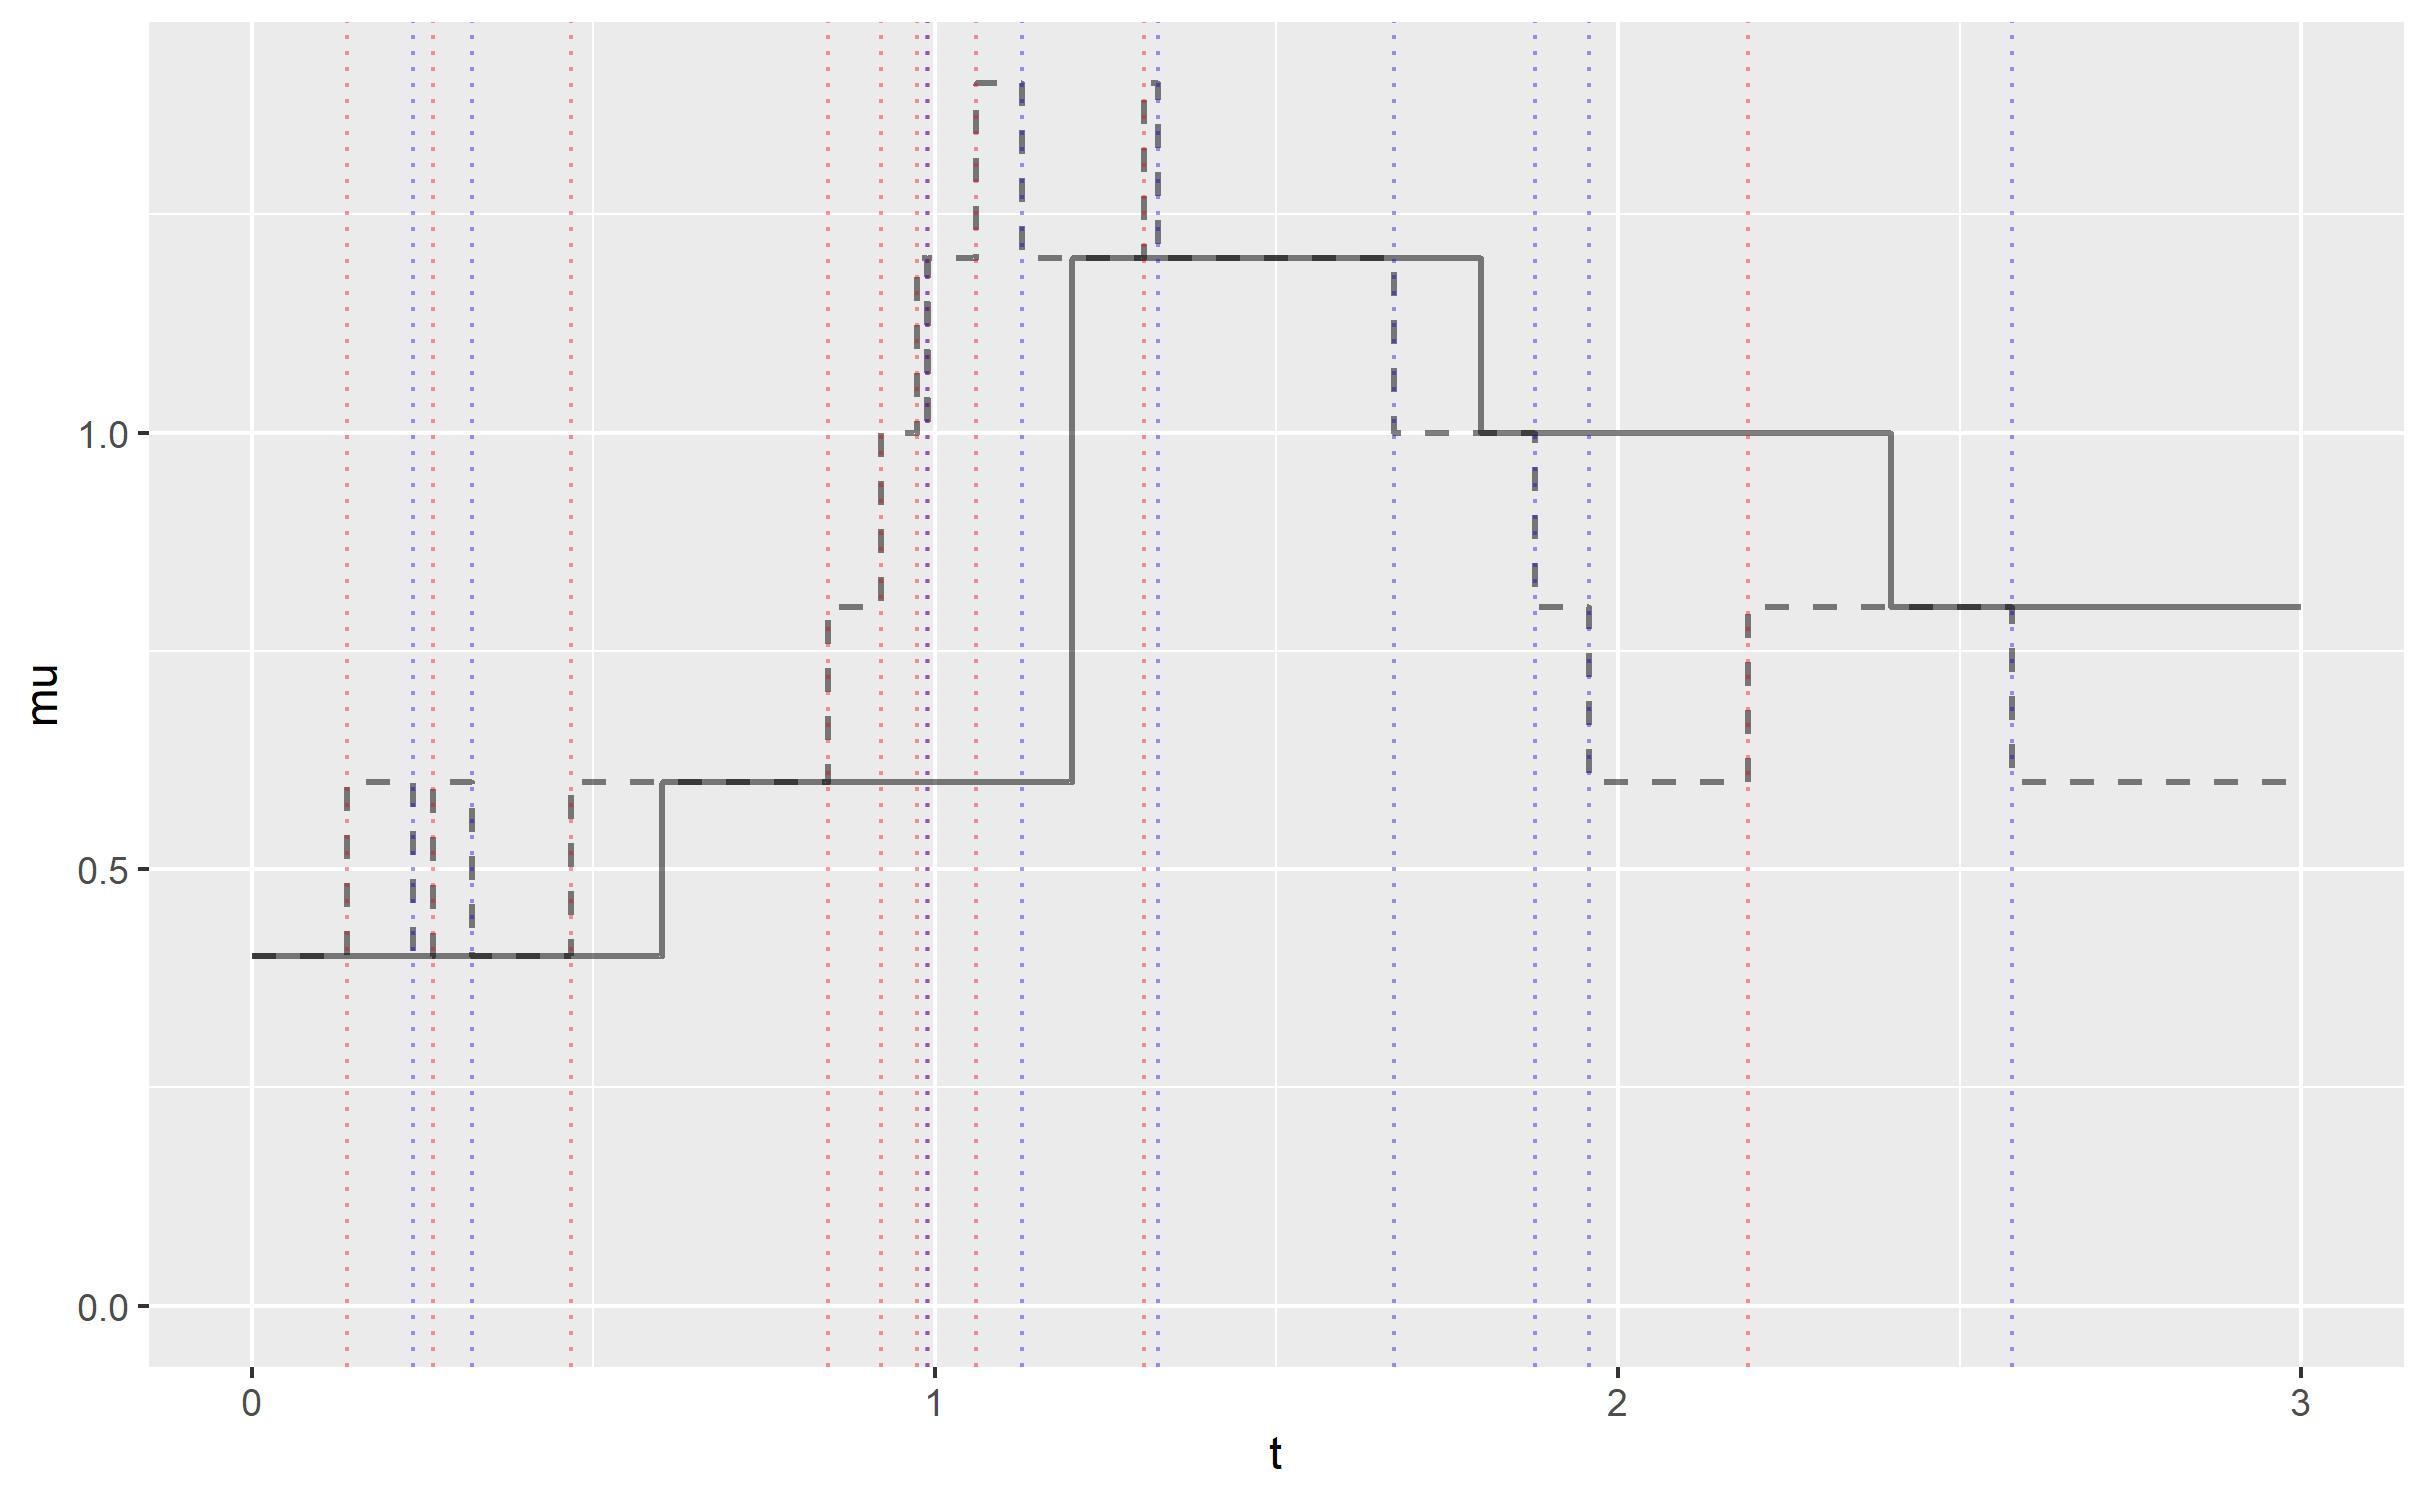
\includegraphics[scale = 0.4]{infection_rate_SIR_PDSIR.jpg}
		\caption{Infection dynamics of the SIR (dashed line) and PD-SIR (solid line) processes in a small population ($(S(0), I(0)) = (10,2)$) with $\beta=1$. The schedule of the PD-SIR is $t_{0:3}=(0, 0.2, 0.4, 0.6)$.
		The vertical dotted lines indicate the infection (red) and removal (blue) times.}
		\label{fig:mu}
	\end{figure}
	
	It now becomes straightforward to simulate realizations from the PD-SIR process conditionally on the observations $\Y = I_{1:K}$. By construction, under the PD-SIR model the variable $S(t)$ follows a linear death process (LDP) during each interval with death rate $\mu_k = \beta I(t_{k-1})$. 
	The LDP is a counting process possessing the so-called order statistics property \cite{Neuts.1971}; that is, given the number of events registered on some interval, the event times are distributed as the order statistics of independent and identically distributed (i.i.d.) random variables following, in the case of the LDP, a exponential distribution truncated to that interval.
	\begin{theorem}
		\label{theo:ldp}
		Consider a linear death process with death rate $\mu$ and let $\tau_{1:N} \in (t_l, t_u]$ be the times of the $N$ deaths occurring between times $t_l$ and $t_u$. Then 
		$$\tau_j \,{\buildrel d \over =}\, X_{(j)}, \quad j = 1, \dots, N$$
		where $X_{(j)}$ is the $j^{\text{th}}$ order statistics of $N$ i.i.d.\ random variables following a truncated exponential distribution with rate $\mu$, lower bound $t_l$ and upper bound $t_u$.
	\end{theorem}
	Appendix \ref{app:ldp} contains the proof of this theorem. Generating values from a truncated exponential distribution can be done extremely efficiently with the inverse cumulative distribution function method \cite{Devroye.2006}. 
	
	We can use Theorem \ref{theo:ldp} to generate latent data  $\z = \left\lbrace (z^I_i, z^R_i)\right\rbrace_{i=1}^{n}$ compatible with $\Y = I_{1:K}$ from the PD-SIR process as follows. For each time interval $[t_{k-1}, t_k)$, we compute $\mu_k = \beta I(t_{k-1})$ and $U_k = I(0) + \sum_{l=1}^{k-1} I_l$, the cumulative number of infections that happened before $t_{k-1}$. The index set $\mathcal{I}_k = \{U_k + 1, \dots, U_k + I_k\}$ therefore denotes the $I_k$ individuals infected during the $k$th interval. Note that $I(t_{k-1})$ only depends on past events and can therefore be computed given the PD-SIR process up to time $t_{k-1}$. Algorithm \ref{alg:PD-SIR} provides a simple recursion to compute this variable efficiently. For $j \in \mathcal{I}_k$, following Theorem \ref{theo:ldp}, we sample the infection times $z^I_j \sim \TruncExp(\mu_k; t_{k-1}, t_k)$, a truncated exponential distribution with rate $\mu_k$ bounded between $t_{k-1}$ and $t_k$. For the same indices $j$, we then generate the removal times $z^R_j$ from the removal dynamics of the SIR. To accomplish this, we sample the removal time of individual $j$ from the mixed distribution
	$$z^R_j|z^I_j \sim (1 - p_j) \delta_{\infty} + p_j \TruncExp(\gamma; z^I_j, t_{end})$$
	placing point mass $(1 - p_j)$ at $\infty$ and continuous mass on the interval $(z^I_j, t_{end}]$,
	where $\delta_{\infty}$ corresponds to the Dirac distribution with mass $1$ on the element $\infty$, and
	$$p_j = 1 - \exp\{-\gamma (t_{end} - z^I_j)\} = P(z^R_j \le t_{end} | z^I_j)$$
	is the cumulative distribution function of an exponential distribution with rate $\gamma$. % and corresponds to the probability that particle $j$ is removed before $t_{end}$ given that it was infected at time $z^I_j$,
	
	By construction, this scheme generates latent data from the PD-SIR process that are compatible with $\Y = I_{1:K}$. The density $q$ of the proposal kernel $Q$ for the PD-SIR process corresponds to
	\begin{alignat}{3}
	\label{eq:q}
		q(\z|\theta) 
		& = && \prod_{k=1}^K \prod_{j\in\mathcal{I}_k} \TruncExp(z^I_j; \mu_{k}, t_{k-1}, t_{k}) \\
		& && \times \prod_{i=1}^{n} \left( 1 - p_i \right)^{\mathbf{1}(z^R_i = \infty)} \left( p_i \TruncExp(z^R_i; \gamma, z^I_i, t_{end}) \right)^{\mathbf{1}(z^R_i \le t_{end})}
	\end{alignat}
	where %$\mu_k = \beta I(t_{k-1})$ and
	$$\TruncExp(x; \mu, l, u) = \dfrac{\mu \exp\{-\mu x\}}{\exp\{-\mu l\} - \exp\{-\mu u\}}, \quad x \in (l, u)$$
	denotes the density of a truncated exponential distribution with parameters as notated previously. Algorithm \ref{alg:PD-SIR} provides a summary of the proposal scheme in pseudo-code.
	
	\begin{algorithm}
		\caption{Generating a PD-SIR process conditionally on the observed data $\Y = I_{1:K}$}
		\label{alg:PD-SIR}
		\begin{algorithmic}
			\REQUIRE $I_{1:K}, \theta = (\beta, \gamma)$, $I(0)$
			\FOR {$j = 1, \dots, I(0)$}
    			\STATE $z^I_j \leftarrow 0$ (by the memoryless property of the exponential distribution).
    			\STATE $p_j \leftarrow 1 - \exp\{-\gamma (t_{end} - 0)\}$
    			\STATE $z^R_j \sim (1 - p_j) \delta_\infty + p_j \TruncExp(\gamma, 0, t_{end})$
			\ENDFOR
			
			\FOR {$k = 1, \dots, K$}
    			\STATE $U_k \leftarrow I(0) + \sum_{l=1}^{k-1} I_l$
    			\STATE $\mathcal{I}_k \leftarrow \{U_k + 1, \dots, U_k + I_k\}$
    			\STATE $\mu_k \leftarrow \beta I(t_{k-1})$
    			\STATE $X_{\mathcal{I}_k} \sim \TruncExp(\mu_k, t_{k-1}, t_k)$ i.i.d.\
    			
    			\FOR {$j \in \mathcal{I}_k$}
        			\STATE $z^I_j \leftarrow X_{(j)}$ (infection times)
        			\STATE $p_j \leftarrow 1 - \exp\{-\gamma(t_{end} - z^I_j)\}$
        			\STATE $z^R_j \sim (1 - p_j) \delta_\infty + p_j \TruncExp(\gamma, z^I_j, t_{end})$ (removal times)
    			\ENDFOR
    			\STATE $R_k \leftarrow \#\{i:\tau^R_i \in (t_{k-1}, t_k]\}$ (number of removals in the $k^{\text{th}}$ interval)
    			\STATE $I(t_k) \leftarrow I(t_{k-1}) + I_k - R_k$
			\ENDFOR
		\end{algorithmic}
	\end{algorithm}
	
	The following four characteristics of our DA-MCMC algorithm are worth noting.
	First, initializing the Markov chain only requires values for the initial parameters $\theta^{(0)} = (\beta^{(0)}, \gamma^{(0)})$ since $\Z^{(0)}$ can be generated conditionally on $\Y$ and $\theta^{(0)}$ alone from the PD-SIR process.
	Second, since the PD-SIR closely approximates the SIR model, the acceptance rate in the MH step for the latent data is typically high. For large populations, however, the acceptance rate may drop considerably, thereby hindering the mixing of the Markov chain. To address this issue, we introduce a tuning parameter $\rho \in (0, 1]$ which determines the proportion of individuals whose trajectory is updated per iteration. That is, in a given MH step, we only update the infection and removal times of a subset of $\lceil\rho n\rceil$ individuals chosen uniformly at random.
	Smaller values for $\rho$ result in smaller jumps in the latent space and a larger MH acceptance rate, which may lead to better overall mixing in large populations.
	Third, if all event times are updated ($\rho = 1$), then the proposed and current latent data are independent conditionally on the current values of the parameters: $\Z^{(k-1)} \perp \Z^* | \theta^{(k)}$. Our proposal scheme can therefore be said to be semi-independent, a characteristic that is crucial for proving the uniform ergodicity of the resulting Markov chain (see Section \eqref{sec:uni}). This contrasts with existing DA-MCMC algorithms which only update a small fraction of the latent data per iteration and generate consecutive configurations of the latent data that are mostly identical. 
	Moreover, since the dimension of the latent data remains constant across iterations in our approach, we do not need to rely of reversible jump MCMC unlike \cite{Gibson.1998} and \cite{ONeill.1999}.
	%Fourth, since the latent data are generated from a process that only resembles the SIR model, we ensure that the Markov chain converges to the correct distribution $\pi(\theta, \Z|\Y)$ by proposing and accepting the latent data according to a Metropolis-Hastings scheme. This results in exact Bayesian inference targeting the posterior distribution under the original SIR model.
	%Even though the latent spaces are generated from an approximation of the SIR process, the Metropolis-Hastings step ensures that the Markov chain converges to the posterior distribution of the parameters under the SIR model; in other words, the inference is exact.
	Finally, not only is proposing latent data from the PD-SIR process extremely fast since all the necessary random variables can be generated with the inverse cumulative distribution function method, but ensuring that the proposed latent data are compatible with the observed data can be done at no additional cost, making the proposal scalable to large outbreaks.
	
	\subsection{Quality of Approximation}
	\label{sec:qua}
	% Outline: spaghetti plot, compare distribution of a particular infection time under SIR v approximation process (plot density and compute KS distance).
	
	In the special case $\rho=1$, the latent data proposal is independent of the current configuration of the latent data. The efficiency of the DA-MCMC algorithm to explore the latent space is therefore directly related to the acceptance rate of the MH step, which in turn depends on how faithfully the surrogate process resembles the target process. If the two processes are similar, then the proposed latent data will often be accepted and the Markov chain will have better mixing properties.
	
	The PD-SIR process only differs from the SIR process in its infection dynamics, with the removal dynamics being identical in the two processes. Figure \ref{fig:comparison} compares the trajectories of the compartments $S$, $I$ and $R$ of a SIR process of moderate size ($(S(0), I(0)) = (1000, 10)$ with $(\beta, \gamma) = (0.003, 1)$ and $t_{end} = 6$) and those of four PD-SIR processes constrained to be compatible with the observed incidence data $I_{1:K}$ from the SIR process for $K \in \{5, 10, 50, 1000\}$. We see that the PD-SIR is qualitatively close to the SIR, even for small values of $K$. Unsurprisingly, the quality of the approximation improves as $K$ increases. The seemingly piece-wise linear trajectory of the S compartment in the PD-SIR visible for small $K$ comes from it following a LDP with piece-wise constant death rate. In the limit as $K \rightarrow \infty$, the infection times are effectively known under the PD-SIR and the two processes are equivalent.
	The fact that the PD-SIR faithfully approximates  the SIR, even for moderate $K$, yields a high acceptance rate in the MH step. As a result, our algorithm can make large jumps in the high-dimensional latent space and thus explores it efficiently. 
	
	\begin{figure}
		\centering
		\begin{subfigure}[b]{0.49\textwidth}
			\centering
			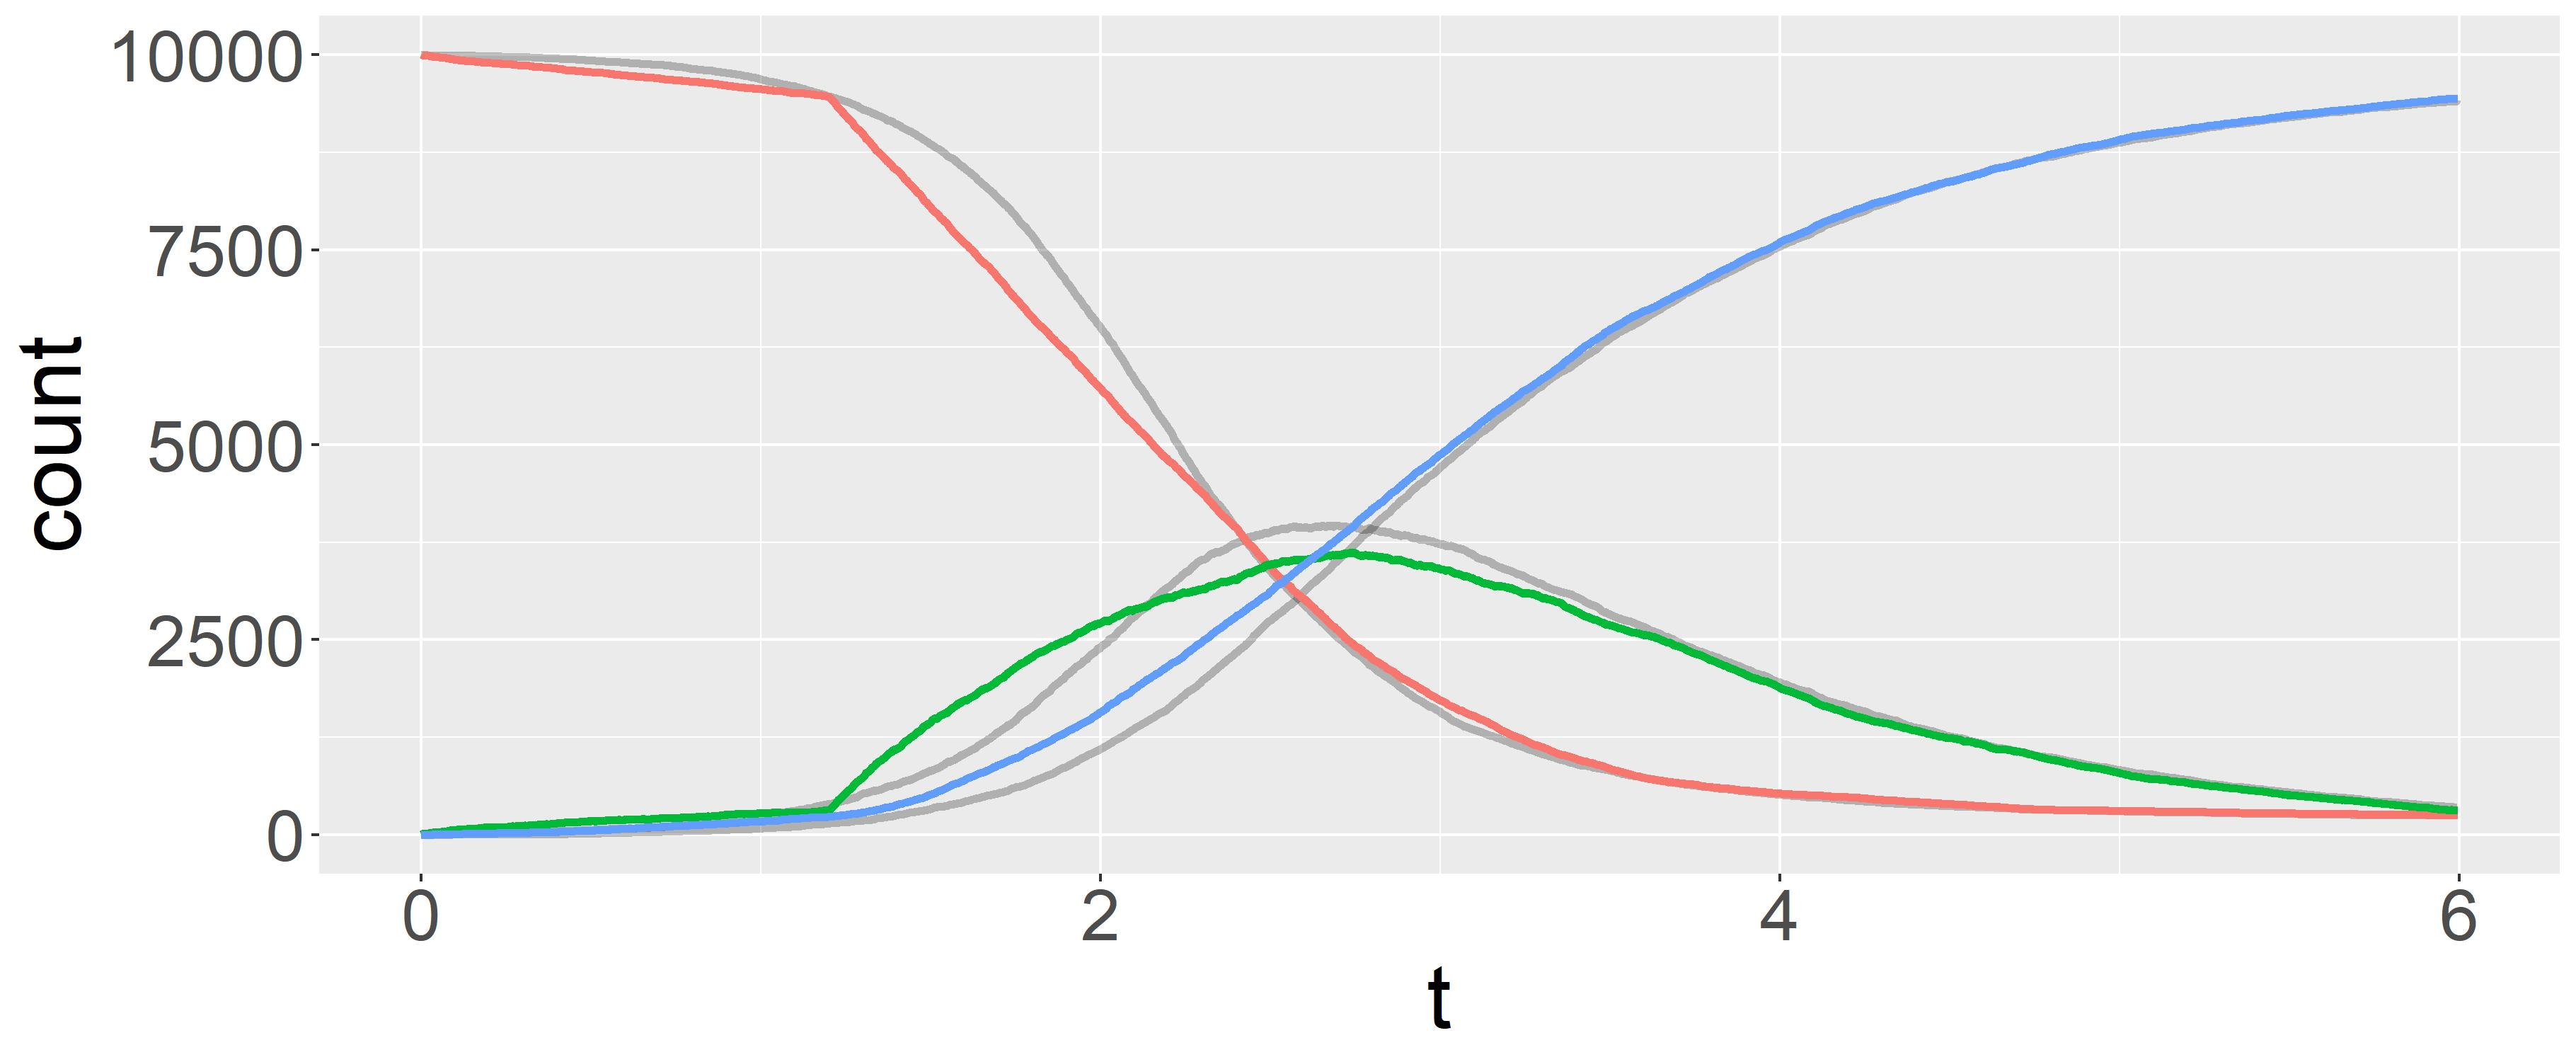
\includegraphics[width=\textwidth]{E2_K5}
			\caption{$K = 5$}
			\label{fig:comparison_RD_SIR_K5}
		\end{subfigure}
		\hfill
		\begin{subfigure}[b]{0.49\textwidth}
			\centering
			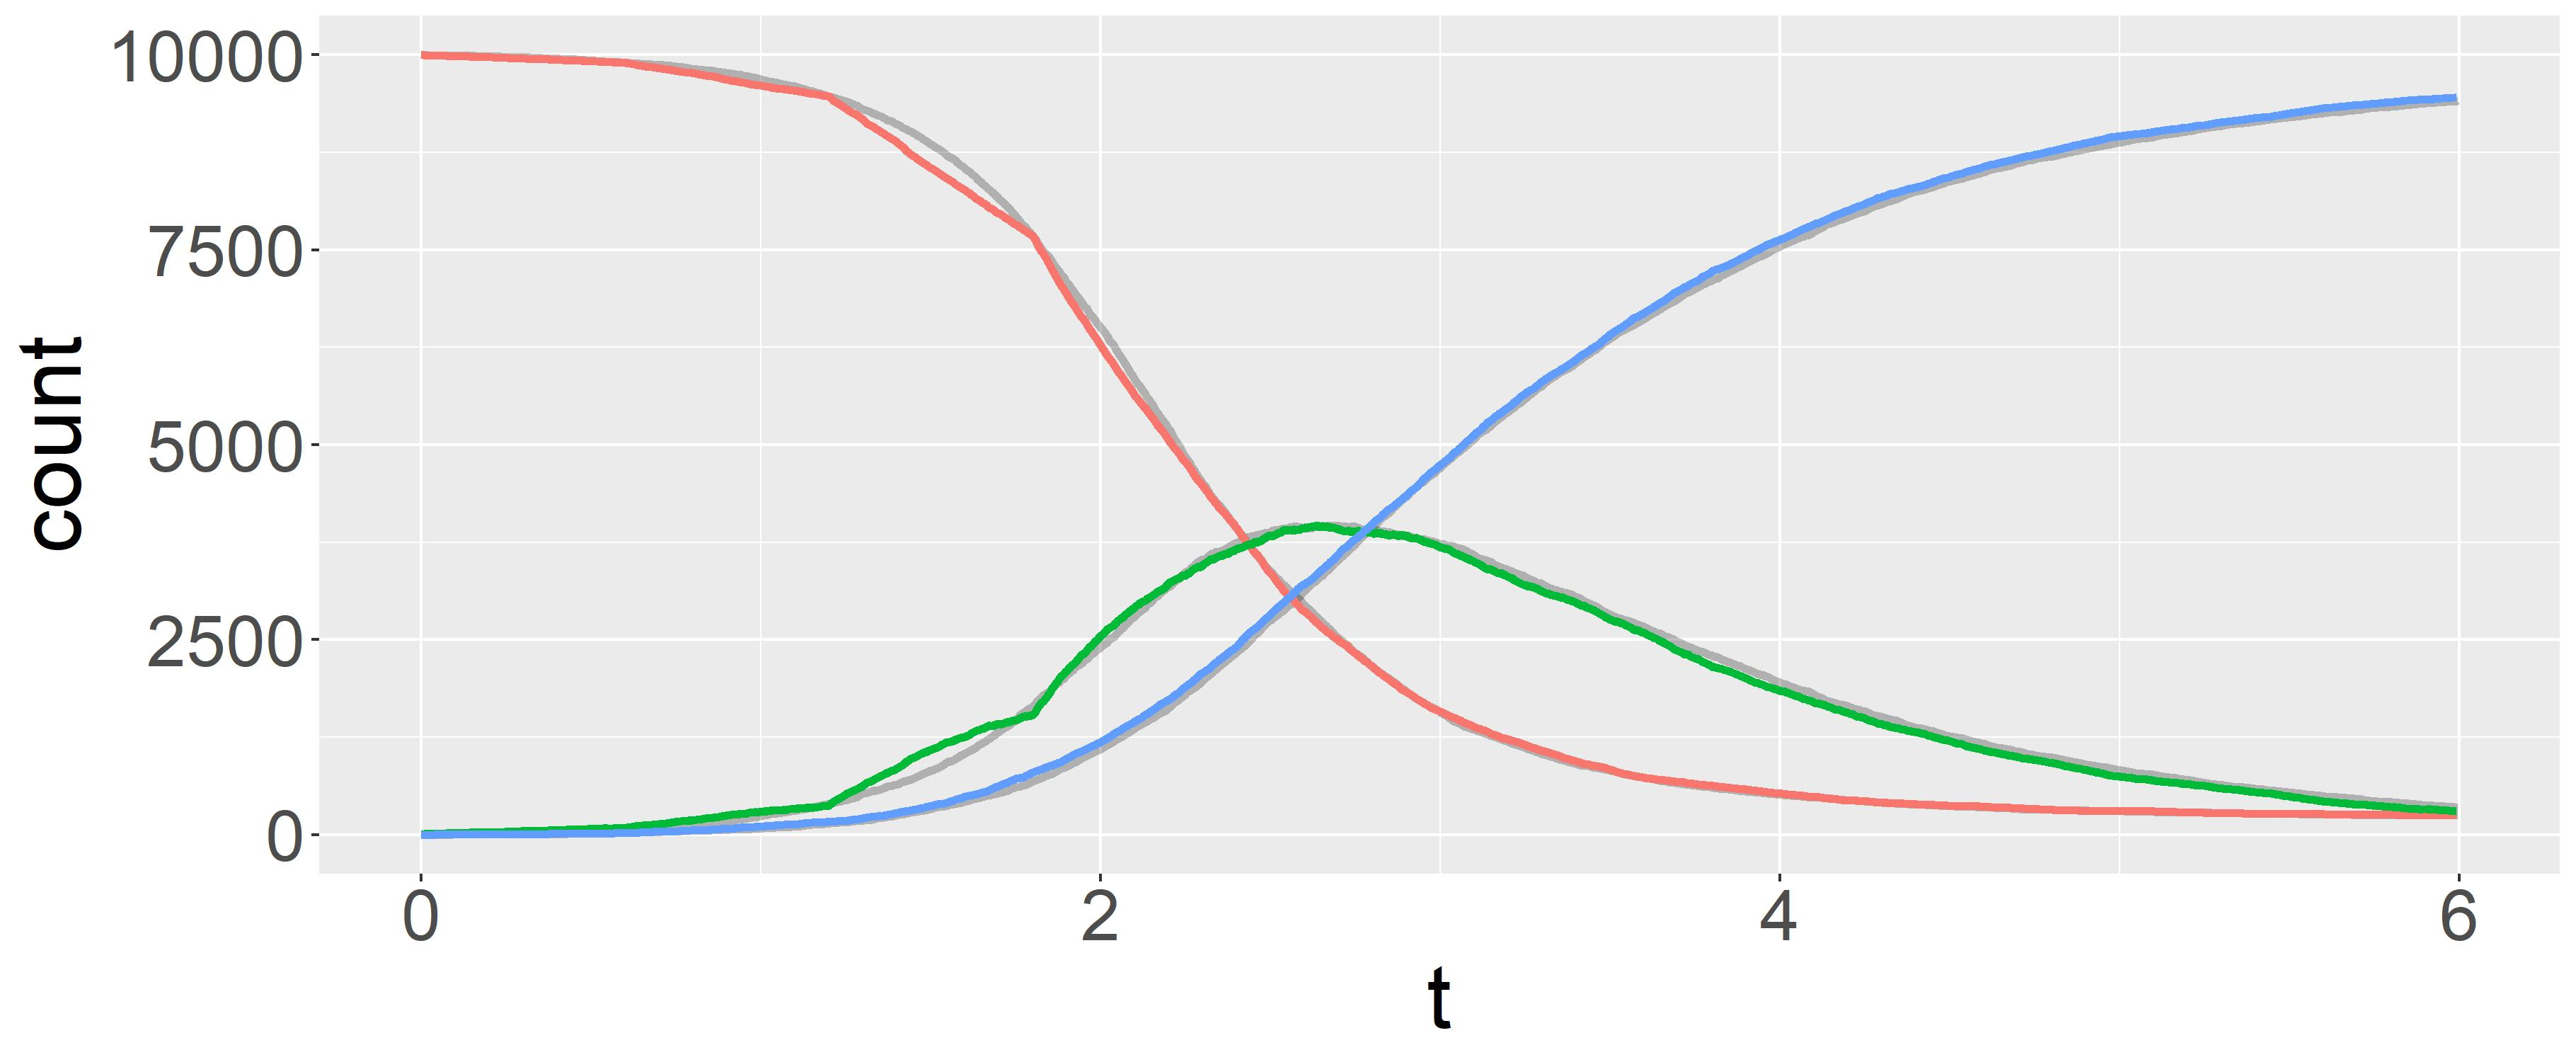
\includegraphics[width=\textwidth]{E2_K10}
			\caption{$K = 10$}
			\label{fig:comparison_RD_SIR_K10}
		\end{subfigure}
		\\
		\begin{subfigure}[b]{0.49\textwidth}
			\centering
			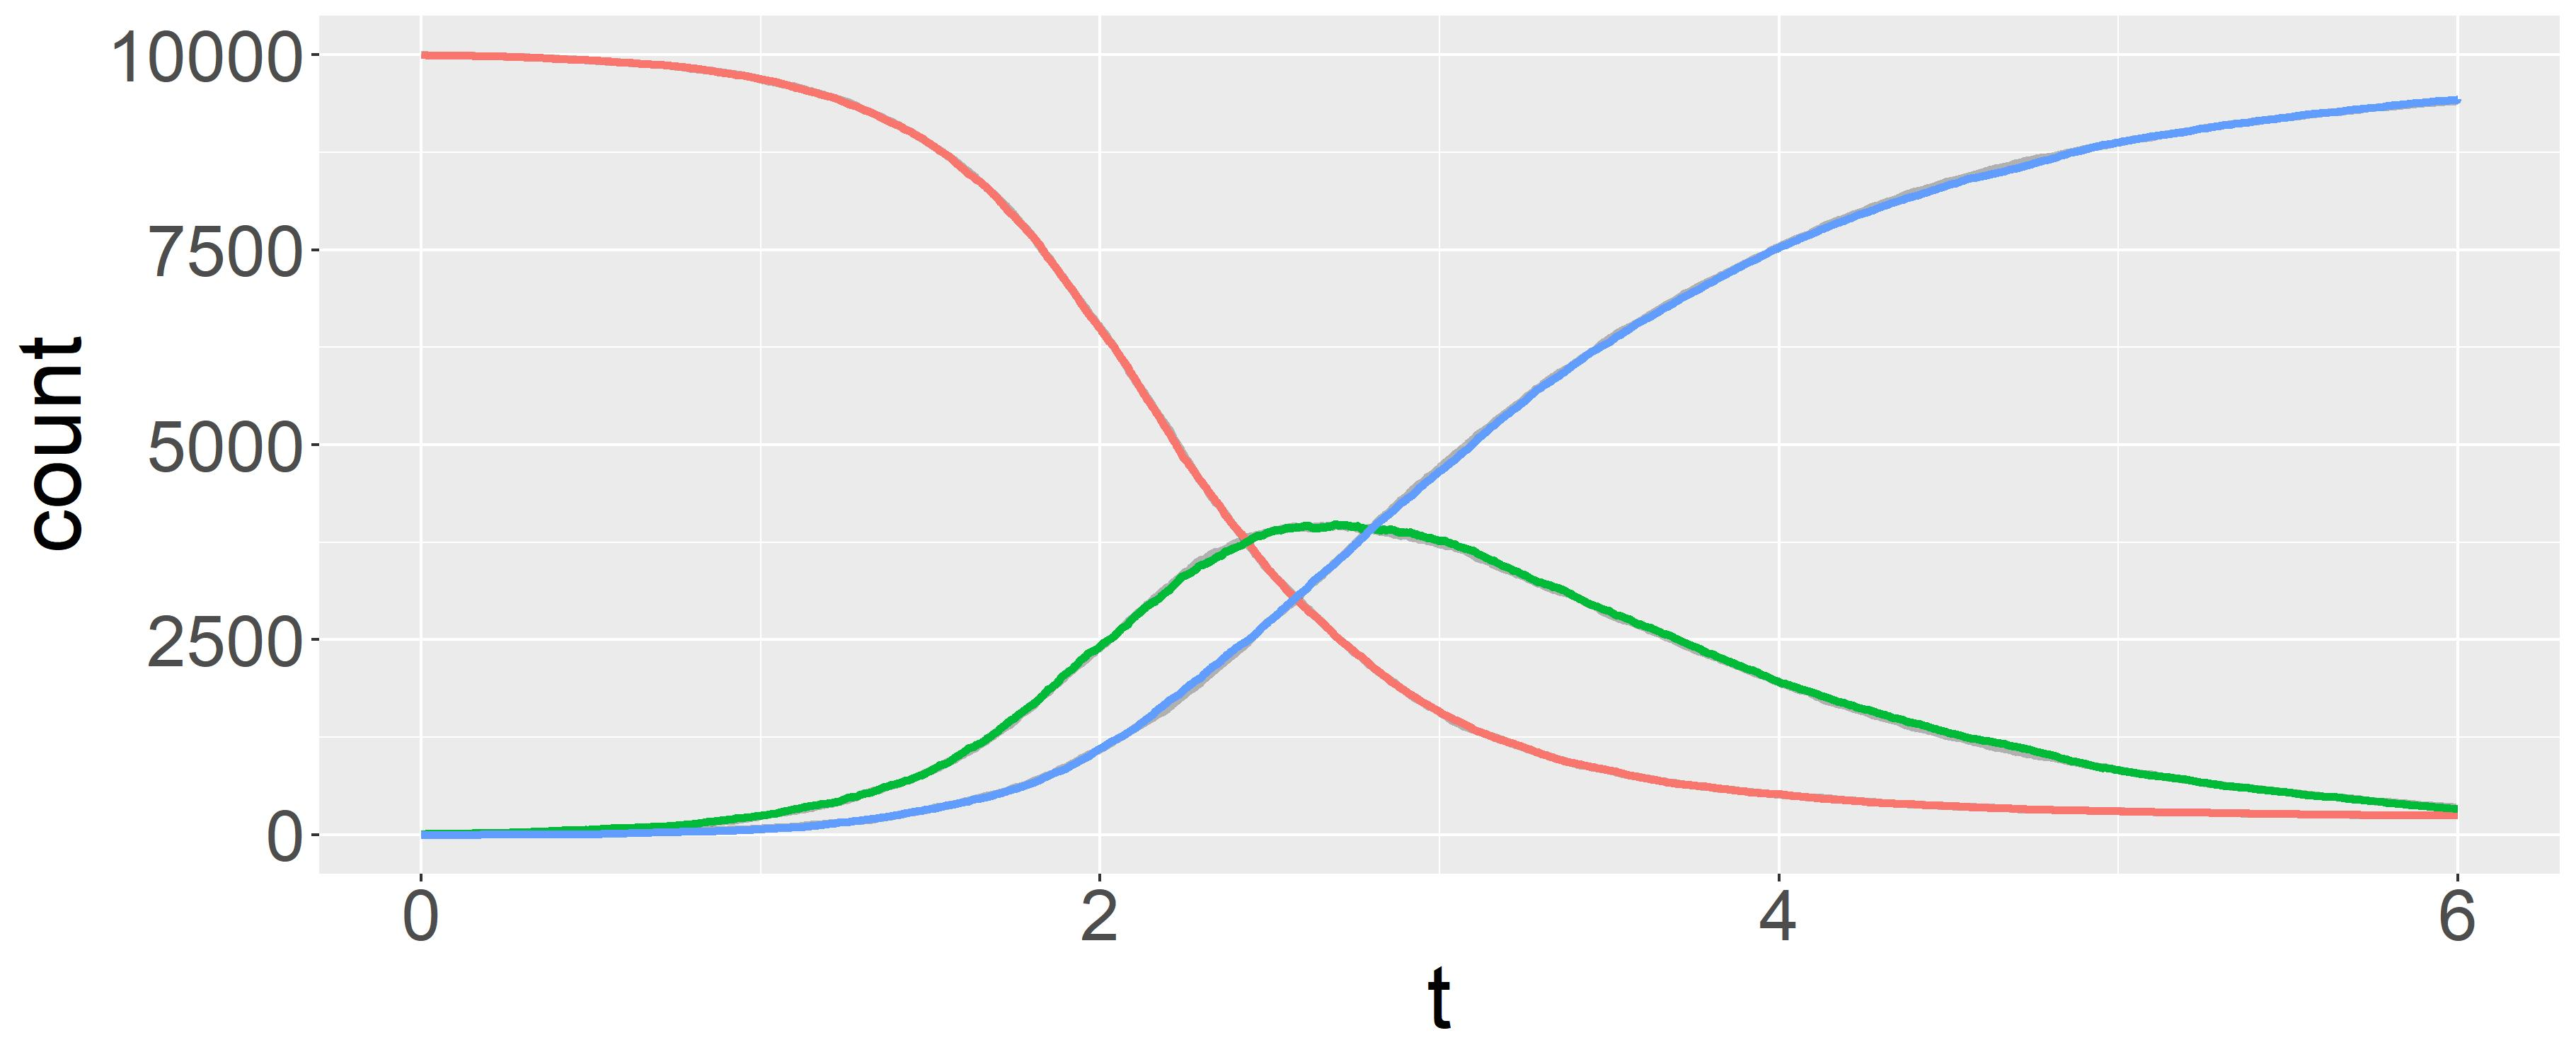
\includegraphics[width=\textwidth]{E2_K50}
			\caption{$K = 50$}
			\label{fig:comparison_RD_SIR_K50}
		\end{subfigure}
		\hfill
		\begin{subfigure}[b]{0.49\textwidth}
			\centering
			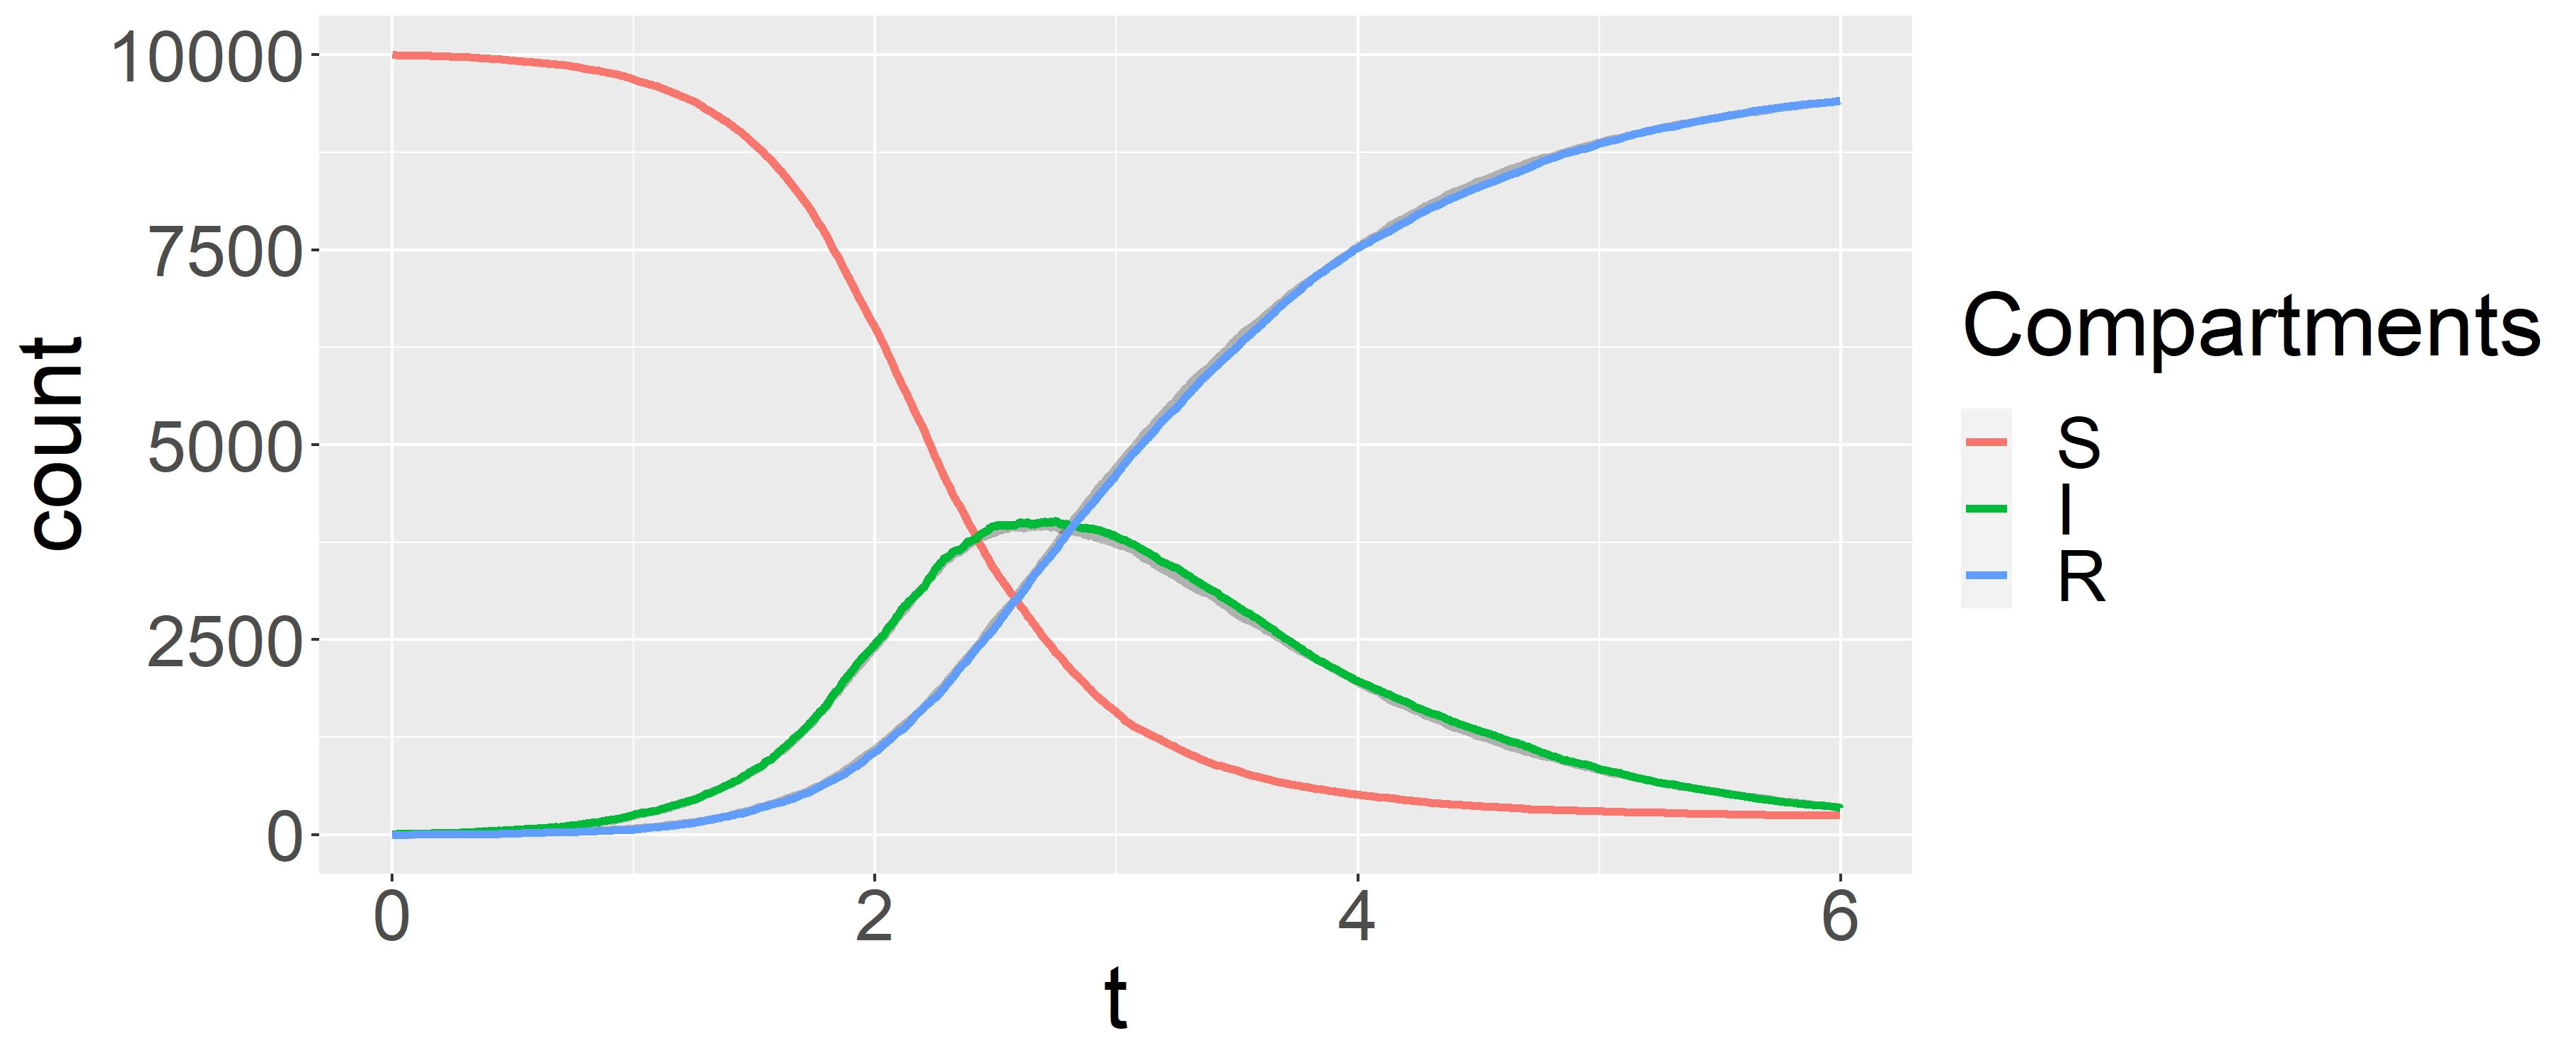
\includegraphics[width=\textwidth]{E2_K1000}
			\caption{$K = 1000$}
			\label{fig:comparison_RD_SIR_K1000}
		\end{subfigure}
		\caption{Trajectories of the compartments $S$, $I$ and $R$ in a SIR (in colors, with $S$ in red, $I$ in green and $R$ in blue) and PD-SIR processes (in grey) with the same infection incidence data $I_{1:K}$.}
		\label{fig:comparison}
	\end{figure}
	\smallskip
	
	\subsection{Uniform Ergodicity}
	\label{sec:uni}
	We now turn to analyze the convergence properties of the Markov chain $\left\{\left(\theta^{(m)}, \z^{(m)}\right)\right\}_m$ underlying the proposed MCMC algorithm. By construction, the joint posterior distribution $\pi(\theta, \z|\Y)$ is invariant for the Gibbs kernel $P_\theta$ that updates $\theta$ and for the MH kernel $P_\z$ updating $\z$, and is therefore also invariant for the composite kernel $P=P_\theta P_\z$ of the MCMC algorithm \cite{Tierney.1994}. Moreover, $P$ is strictly positive, implying that the chain is aperiodic and $\pi$-irreducible. Together with the existence of an invariant distribution, $\pi$-irreducibility implies that the chain is positive Harris recurrent and converges to $\pi(\theta, \z|\Y)$. Hence, for any $\pi$-integrable function $g$, the ergodic theorem holds and the estimator
	$$\bar{g}_m := \frac{1}{m} \sum_{i=0}^{m-1} g\left(\theta^{(m)}, \z^{(m)}\right)$$
	is consistent for $E_\pi g$, for any starting value. 
	
	A Markov chain is said to be \textit{uniformly ergodic} if for some finite $M$ and positive constant $r<1$, the $n$-step transition kernel $P^n$ satisfies
	$$
	\Vert P^n(x,.)-\pi(.)\Vert_{TV} \le M r^n, \quad \forall x \in \chi
	$$
	where $\Vert \mu \Vert_{TV} := \sup_A \mu(A)$ denotes the total variation norm of a signed measure $\mu$.
	Jones \cite{Jones.2004b} shows that uniform ergodicity ensures the existence of a Central Limit Theorem for $\bar{g}_m$ whenever $E_\pi |g|^2 < \infty$. That is,
	$$\sqrt{m}(\bar{g}_m - E_\pi g) \Rightarrow N(0, \sigma^2_g)$$
	for any initial distribution and for some positive, finite $\sigma^2_g$. The constant $\sigma^2_g$ can be estimated via regeneration sampling, batch means or a spectral variance analysis \cite{Flegal.2010}.
	
	Toward establishing the uniform ergodicity of our DA-MCMC algorithm, we will show that the state space $\chi = \chi_{\theta}\times\chi_{\z}$ of the Markov chain $\left\{\left(\theta^{(m)}, \z^{(m)}\right)\right\}_m$ is a \textit{small set} for the transition kernel $P$; that is, there exists a probability measure $\nu$ on the $\sigma$-algebra $\sigma(\chi)$ such that
	\begin{equation}
	\label{eq:uni}
	    P^m(x,.) \ge \epsilon \nu(.), \quad \forall x\in \chi
	\end{equation}
	for a positive integer $m$ and constant $\epsilon > 0$, which holds if and only if the Markov chain is uniformly ergodic \cite{Tierney.1994}.
%	$$
%	\Vert P^n(x,.)-\pi(.)\Vert_{TV} \le M (1-\epsilon)^{n/m}, \quad \forall x \in \chi.
%	$$
	Proposition \ref{pro:uni} shows that \eqref{eq:uni} holds for $m=1$ for our MCMC algorithm when $\rho=1$. This result is worth noting since the requirement that the whole space be small is extremely restrictive and is typically not satisfied for models with unbounded spaces.
	
	\begin{proposition}
		\label{pro:uni}
		For $\rho = 1$, the transition kernel $P$ of the proposed DA-MCMC algorithm satisfies Equation \eqref{eq:uni} with $m=1$, that is,
		$$P((\theta, \z), .) \ge \beta \nu(.) , \quad \forall (\theta, \z) \in \chi_\theta \times \chi_\z
		$$
		for some $\beta>0$ and probability measure $\nu$. As a result $P$ is uniformly ergodic.
	\end{proposition}
	
	We now provide a brief overview of the proof of Proposition \ref{pro:uni} provided in Appendix \ref{app:uni}. Since the kernel $P = P_{\theta} P_{\z}$ is composite, it suffices to minorize $P_\z$ and $P_\theta$ separately. The density of the Gibbs kernel $P_\z$ corresponds to the product of the two gamma densities in \eqref{eq:posterior_theta}; since the sufficient statistics of the latent data are bounded, these gamma densities possess a positive minorization whose closed form is derived in Appendix \ref{app:uni}. Furthermore, the MH kernel $P_\z$ depends on the current latent data only through the ratio $q(\z|\theta)/\pi(\z|\theta)$ which can be bounded above and away from zero.
	
	Finally, it is easy to see that, if $\rho < 1$, Equation \eqref{eq:uni} holds for 
	$m=\lfloor \rho^{-1} \rfloor$ and some $\epsilon$ and $\nu$.
	
	%Since we minorize the transition kernel over the entire state space, the lower bounds we find are not tight. Searching for a better minorization of the form $s(x)\nu(dy)$ and do regeneration sampling (Jones and Hobert, 2001).
	
    %The constant $\epsilon$ that we derive in the proof of Proposition \ref{pro:uni} will in general be too small to be of practical purposes. This results from the loose bounds employed therein. Tighter bounds for the sufficient statistics $\int_{0}^{t_{end}}I(t)dt$ and $\int_{0}^{t_{end}}S(t)I(t)dt$ could be derived by taking into account the observed data $I_{1:K}$. We do not pursue this issue further.
	
	\section{Performance on simulated and real epidemic data}
	\label{sec:per}
	
	\subsection{Simulation Study}
	\label{sec:sim}
	%Outline: (1) proof of concept, (1bis) coverage, (2) rho (3) single-site versus joint proposal
	
	We validate the convergence properties of the proposed DA-MCMC empirically via a suite of simulation studies. First, we assess the performance of the algorithm in a moderately sized population of $1000$ individuals. We simulate an epidemic with true parameters $(\beta, \gamma) = (0.0025, 1)$ -- giving $R_0 = 2.5$ -- starting with $(S(0), I(0)) = (1000, 10)$ until time $t_{end} = 6$, when the outbreak has completed most of its course but is not over yet (see Figure \ref{fig:E1_trajectories}, where $I(t_{end}) = 122$). The numbers of infections in $K = 10$ equal-length time intervals are observed, corresponding to $I_{1:K} = (9, 14, 21, 42, 56, 121, 190, 162, 107, 73)$.	
	We employ the parameterization $\tilde{\theta} = (\beta, R_0)$ and use the semi-conjugate prior distributions \eqref{eq:pri2} with weakly informative hyperparameters $\beta \sim Ga(0.001, 1)$ and $R_0 \sim IG(1,1)$.
	To evaluate the convergence speed of the Markov chain, we initialize it in a low density region at $\left(\beta^{(0)}, \gamma^{(0)}\right) = \left(\beta/10, \gamma/10\right)$. We keep every tenth draw for storage reasons and set $\rho = 0.2$, updating the trajectories of $\lceil\rho n\rceil = 202$ individuals in each MH step.
	
	\begin{figure}
		\centering
		\begin{subfigure}[b]{0.32\textwidth}
			\centering
			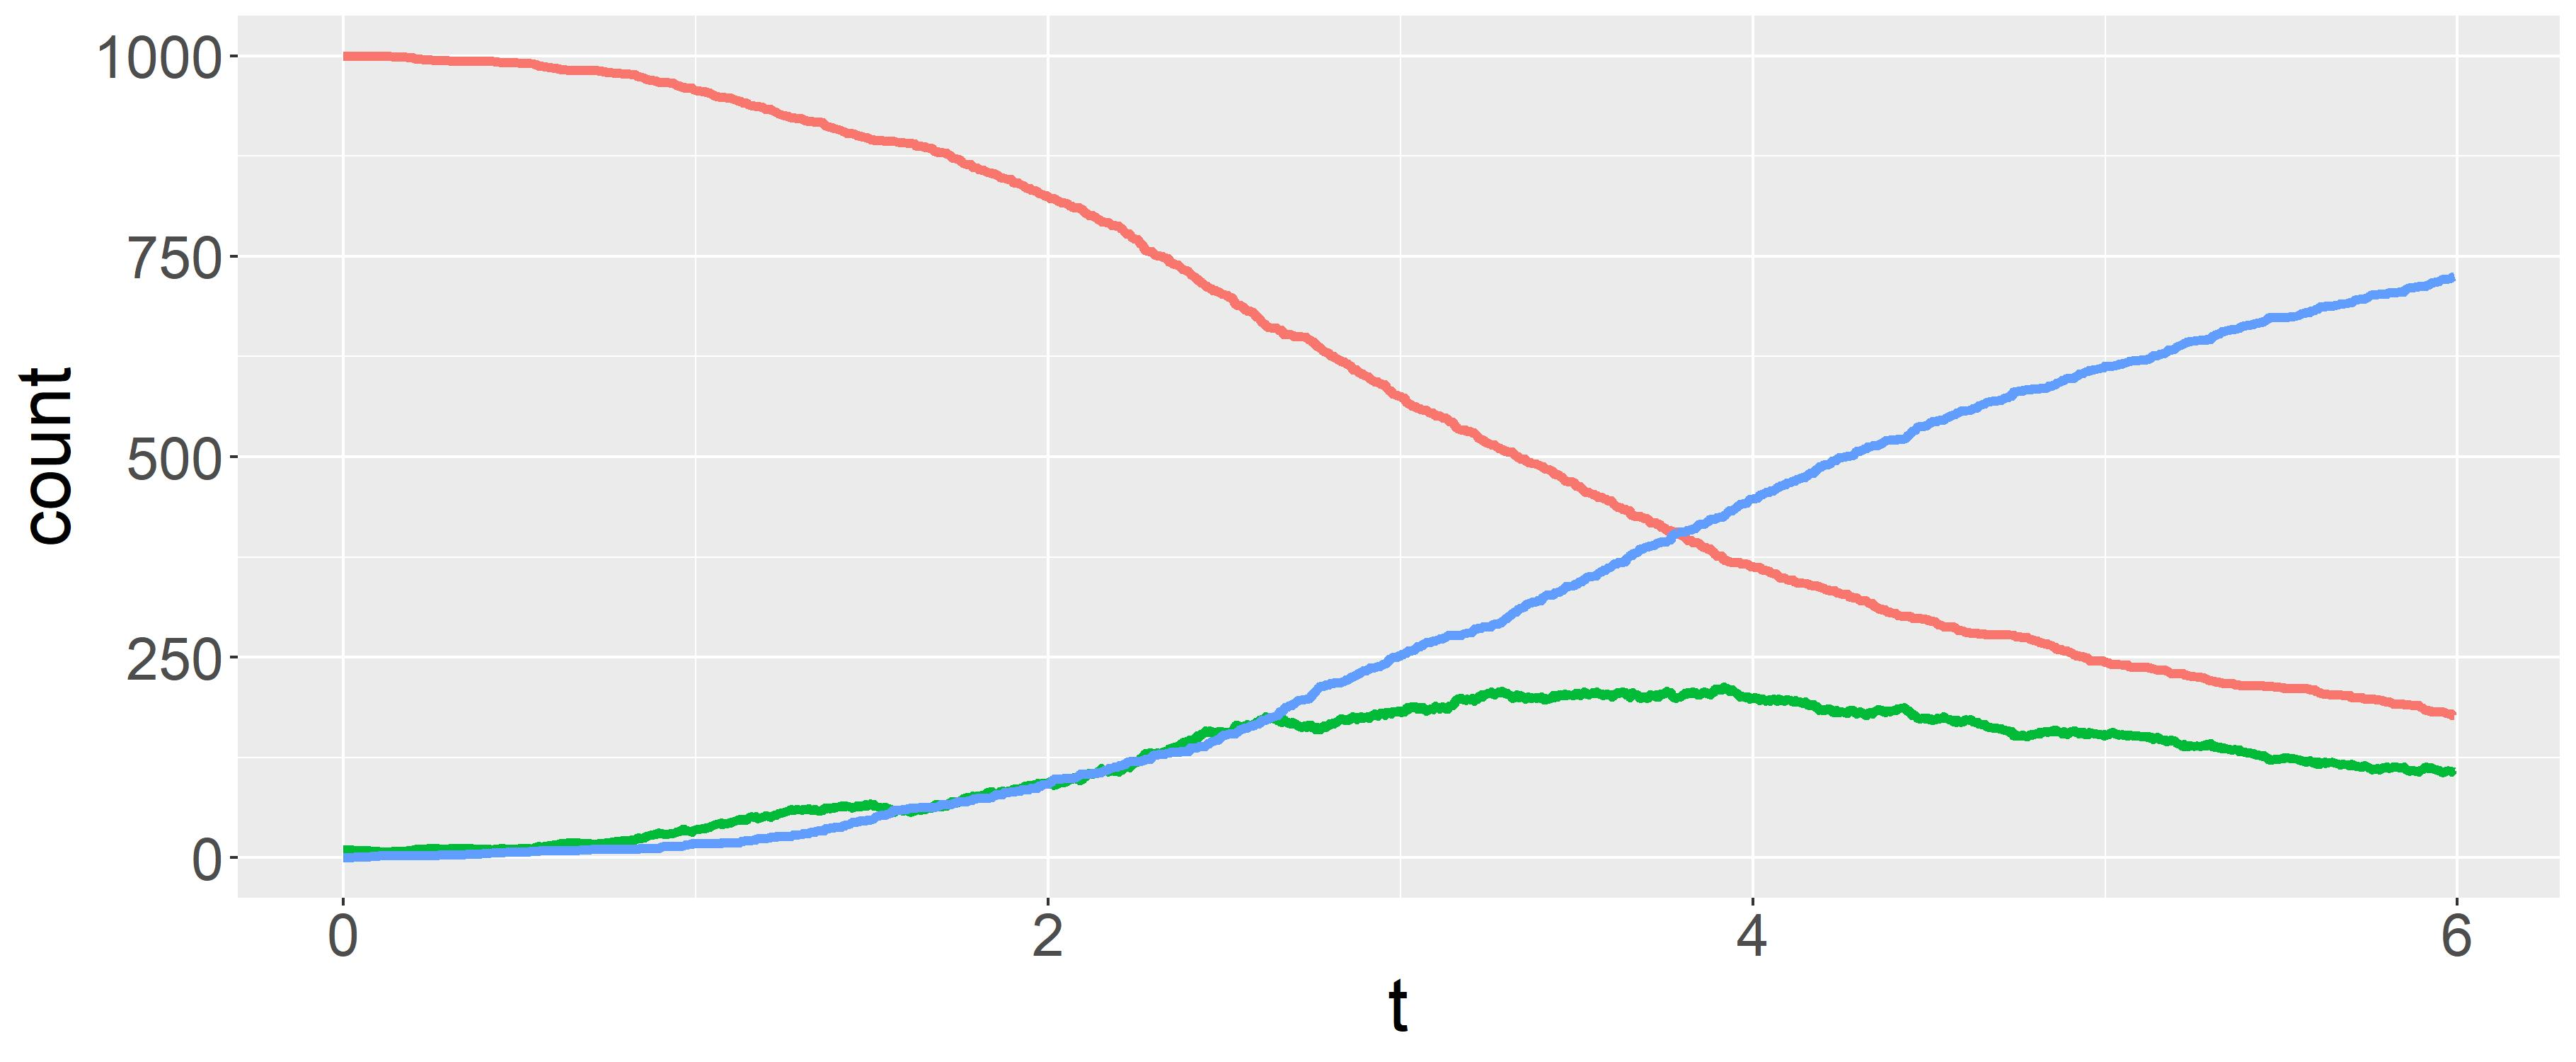
\includegraphics[width=\textwidth]{E1_trajectories}
			\caption{Compartment trajectories ($S$ in red, $I$ in green and $R$ in blue)}
			\label{fig:E1_trajectories}
		\end{subfigure}
		\hfill
		\begin{subfigure}[b]{0.32\textwidth}
			\centering
			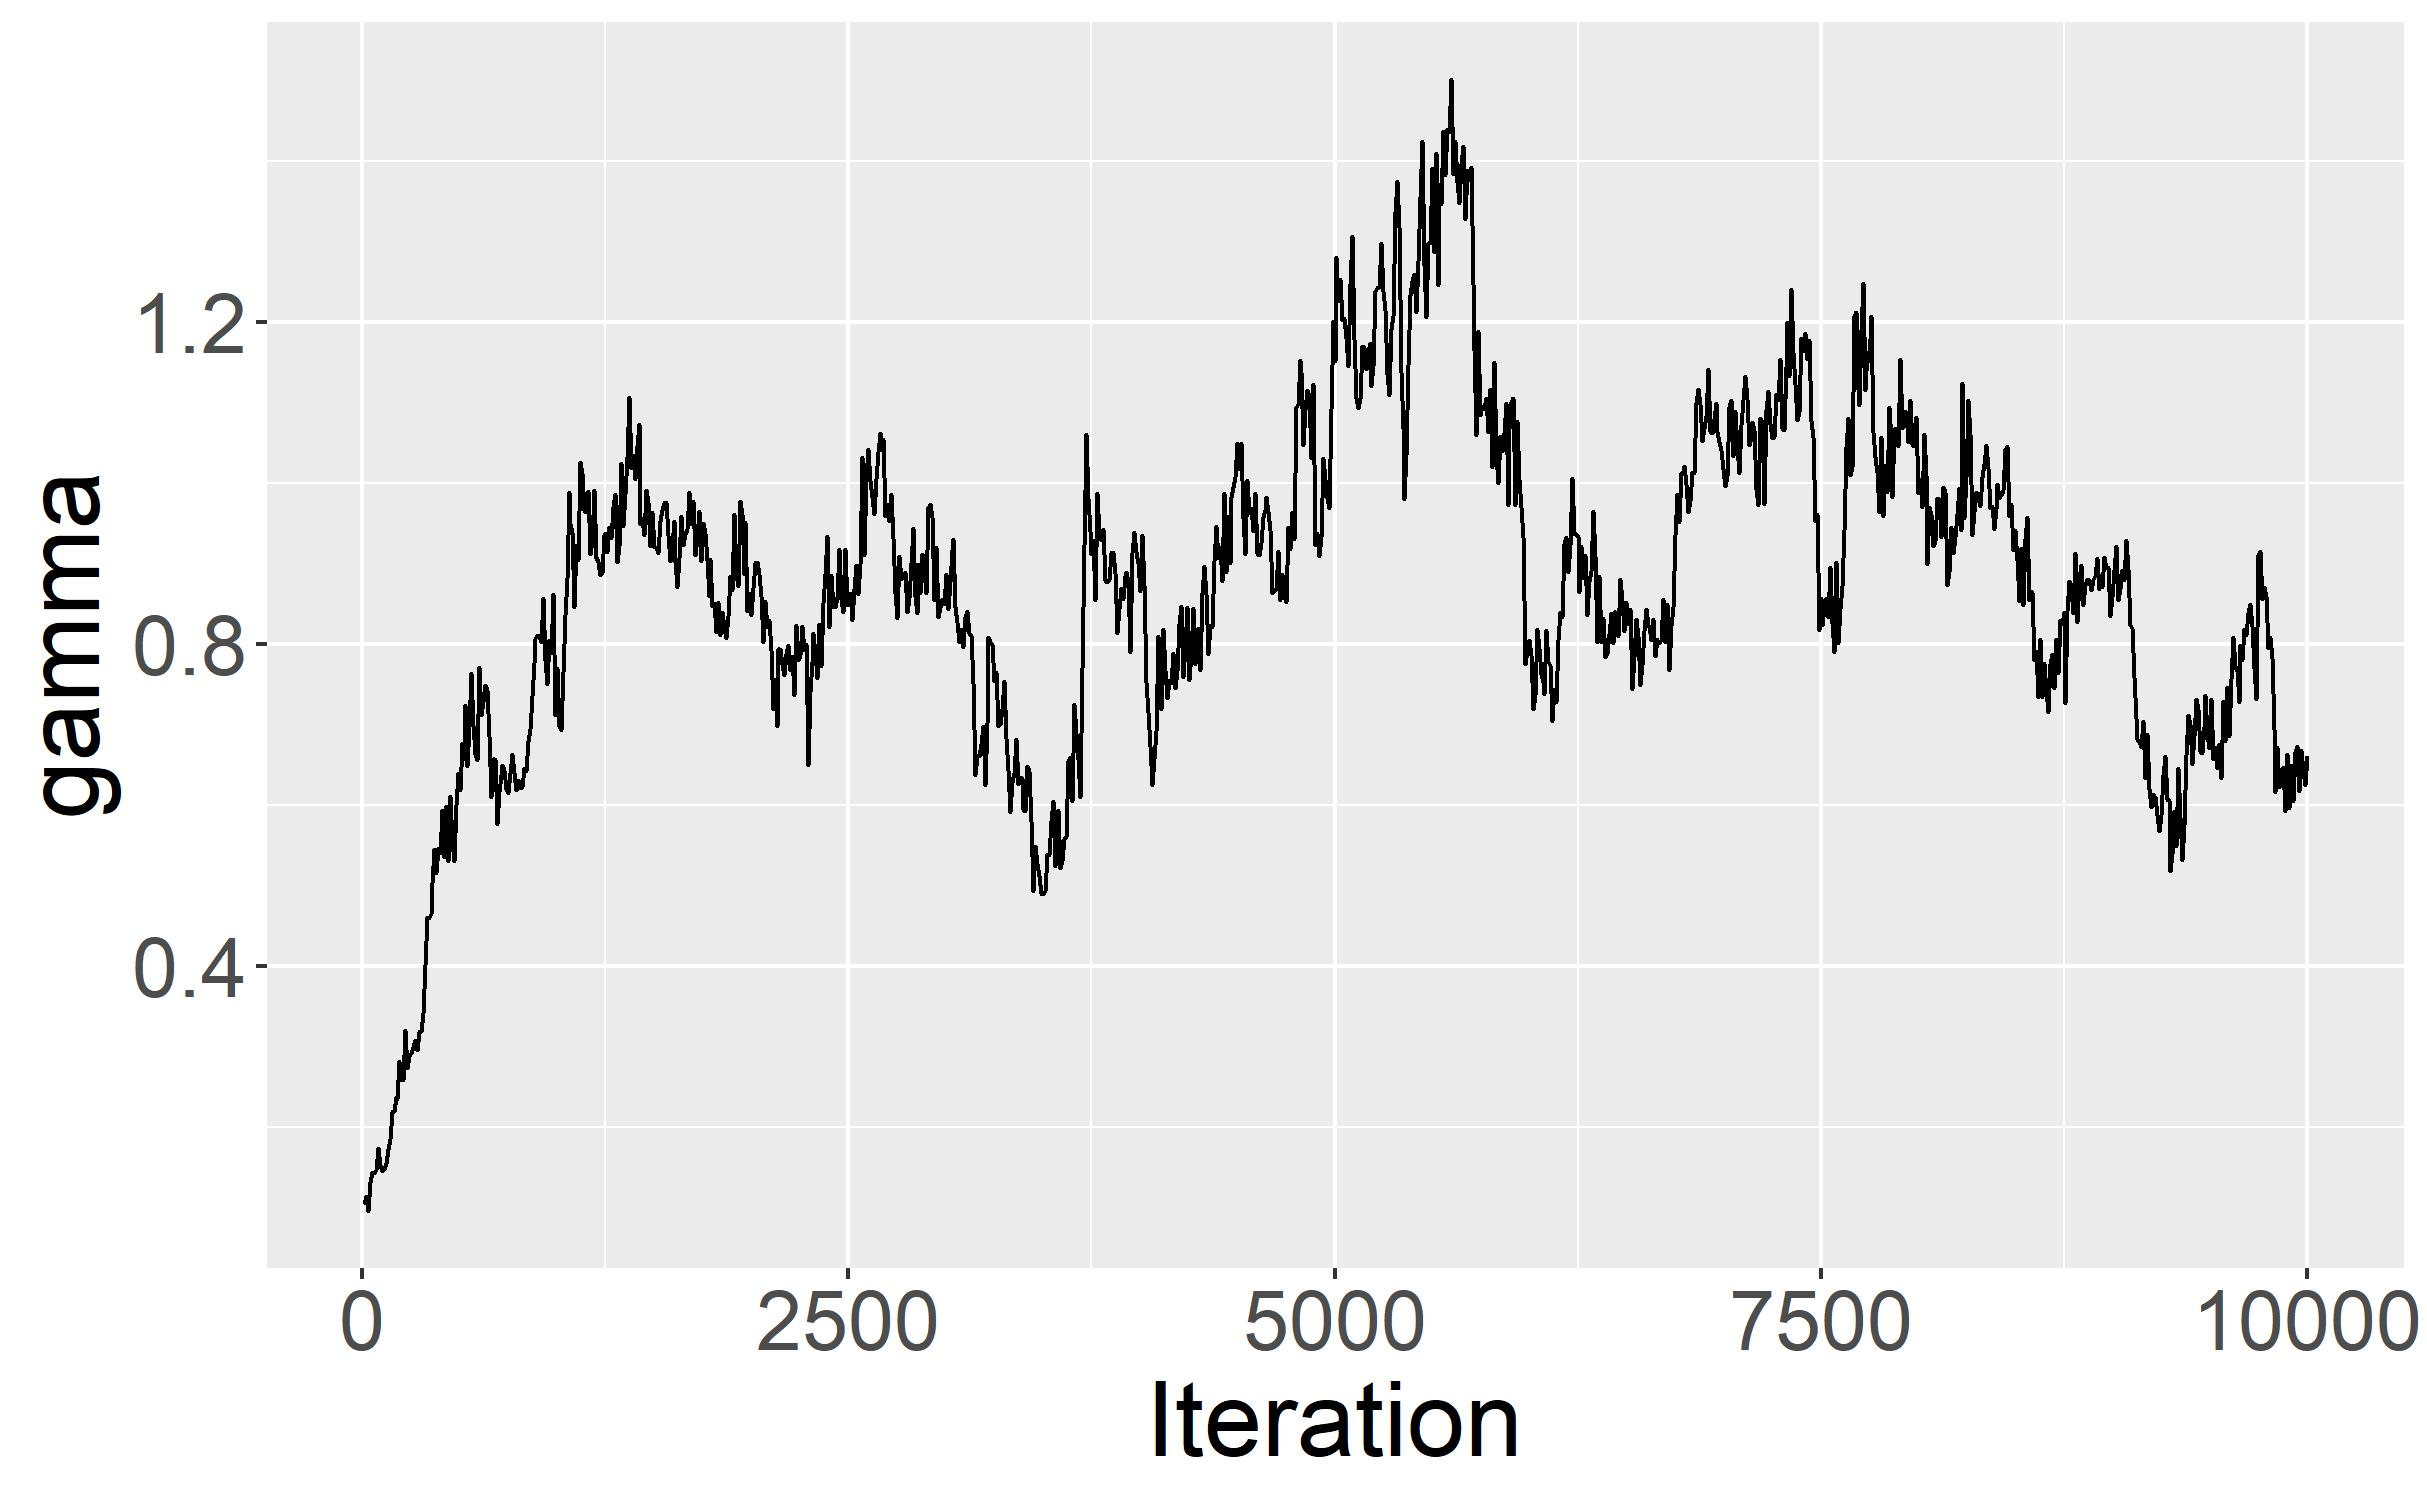
\includegraphics[width=\textwidth]{E1_short_no_burn_gamma_tp}
			\caption{Traceplot during the transient phase}
			\label{fig:E1_short_no_burn_gamma_tp}
		\end{subfigure}
		\hfill
		\begin{subfigure}[b]{0.32\textwidth}
			\centering
			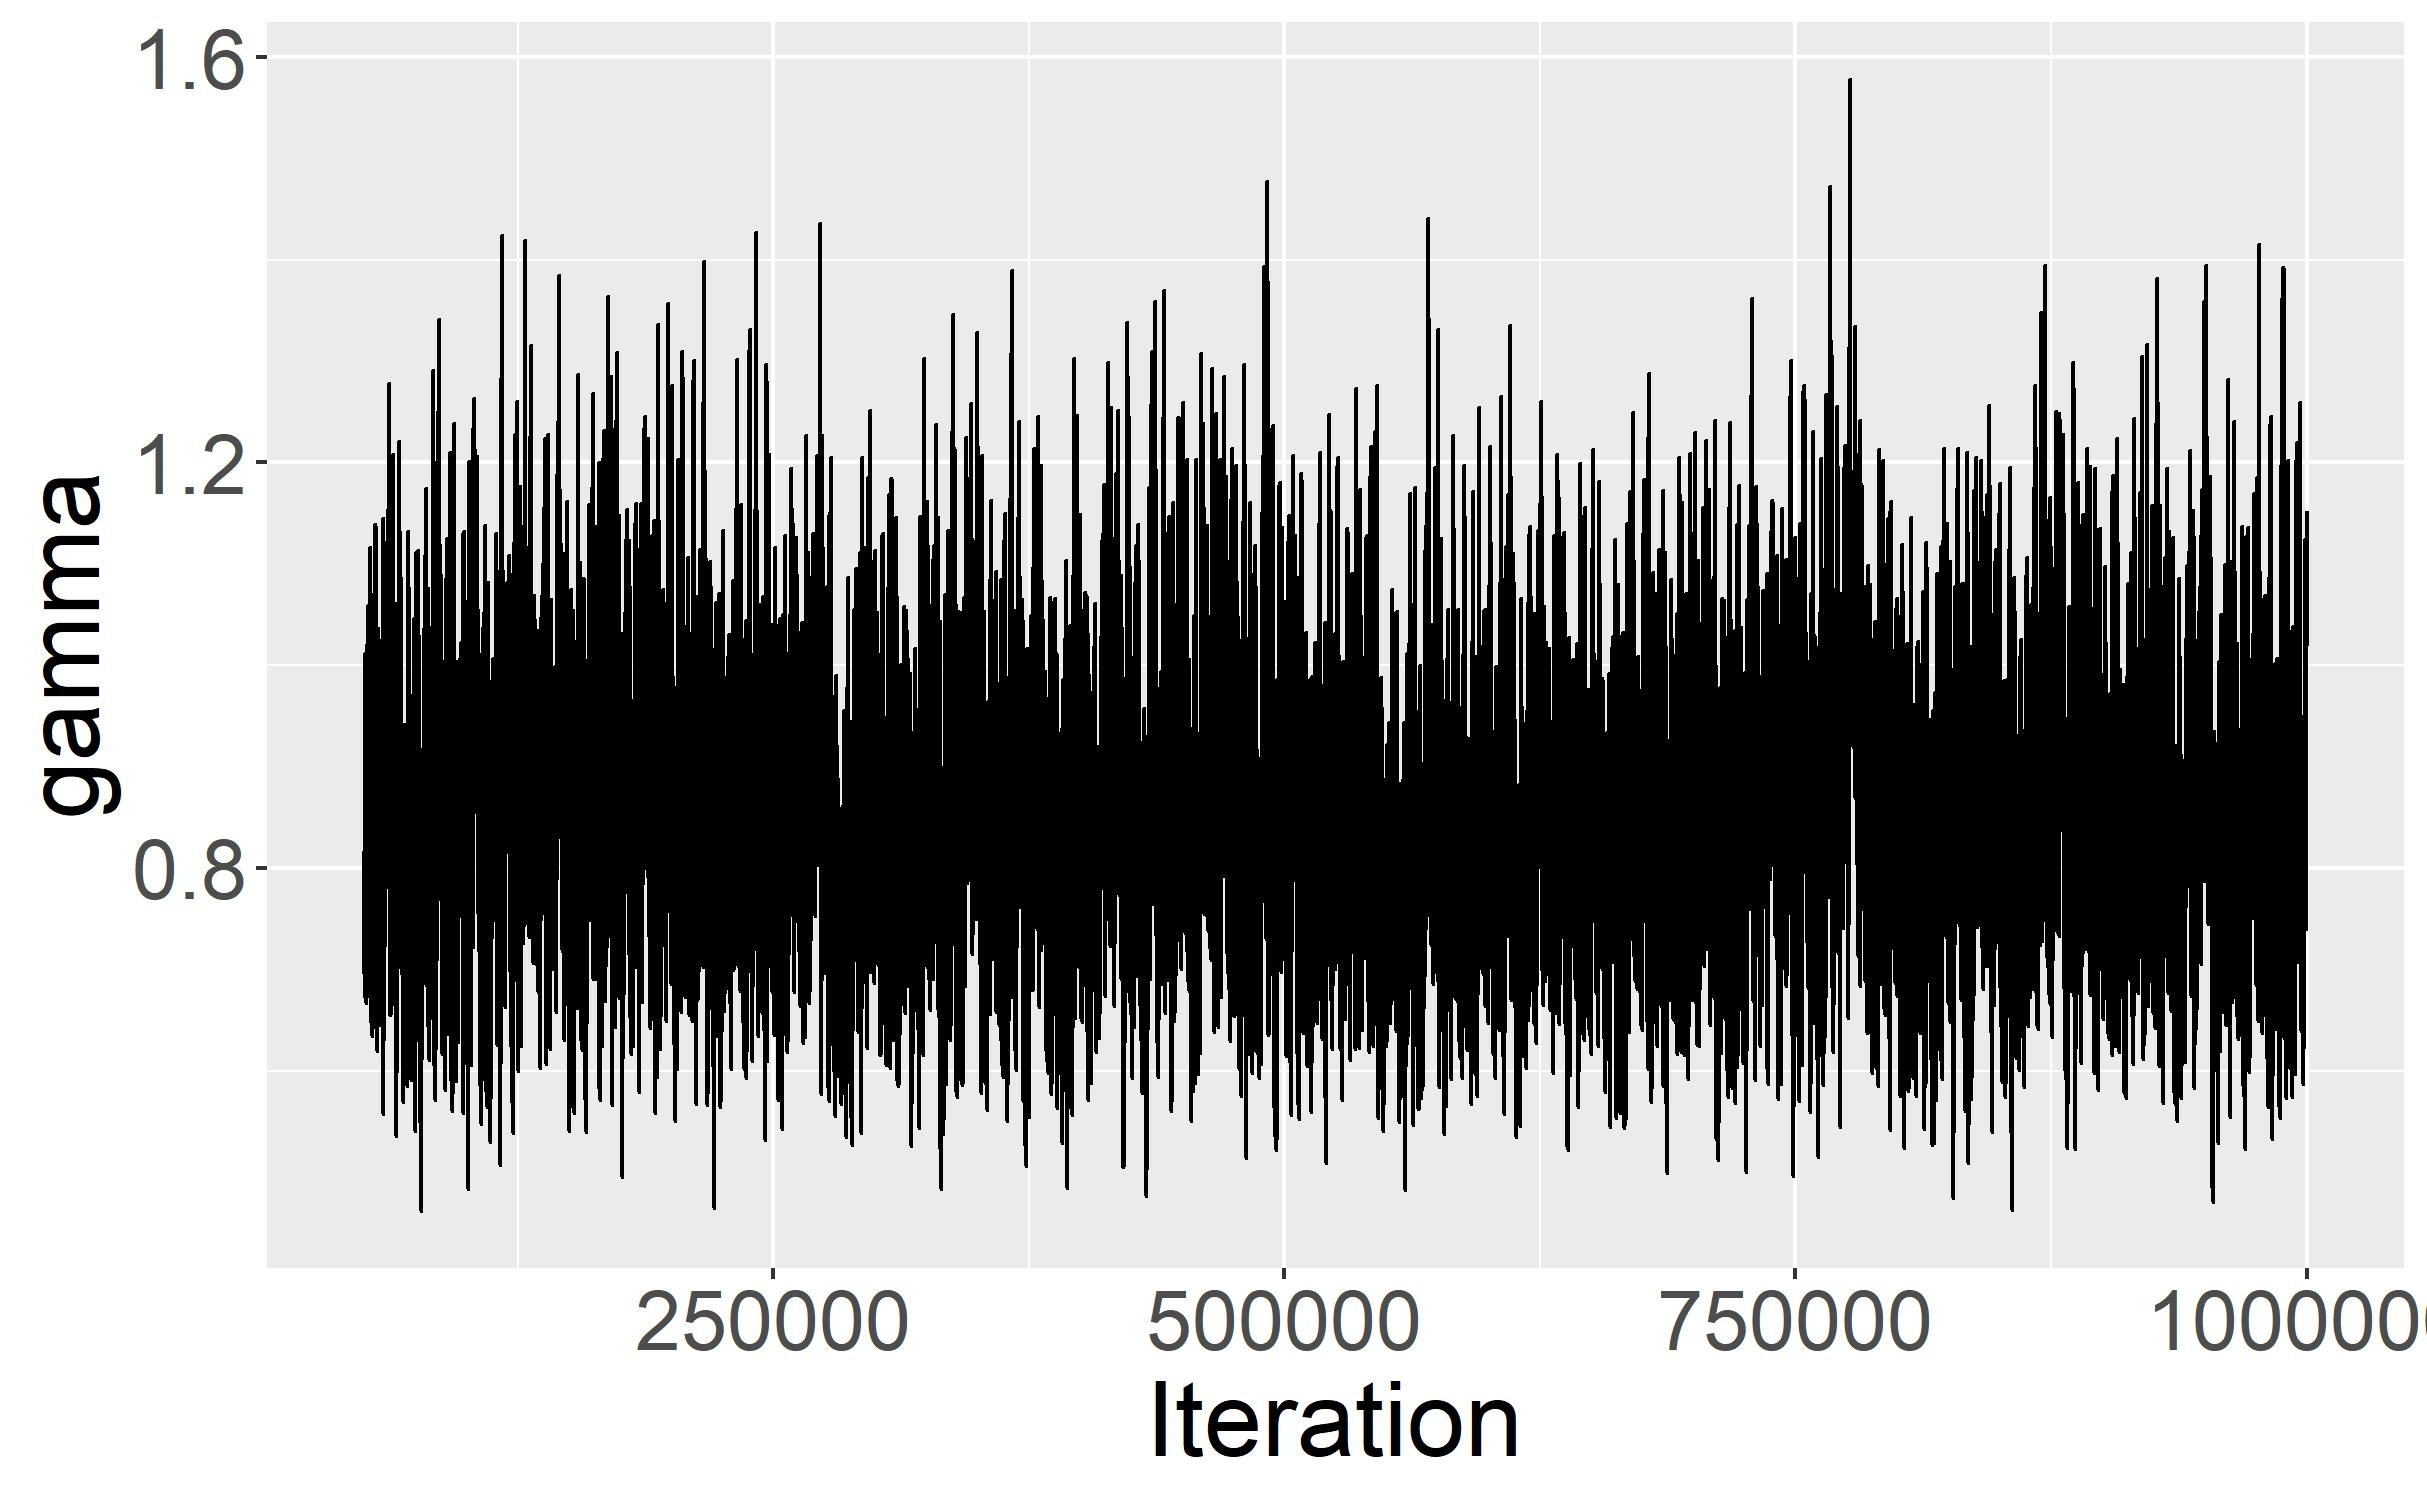
\includegraphics[width=\textwidth]{E1_burn_gamma_tp}
			\caption{Traceplot after the transient phase}
			\label{fig:E1_burn_gamma_tp}
		\end{subfigure}
		%\hfill
		%\begin{subfigure}[b]{0.24\textwidth}
		%	\centering
		%	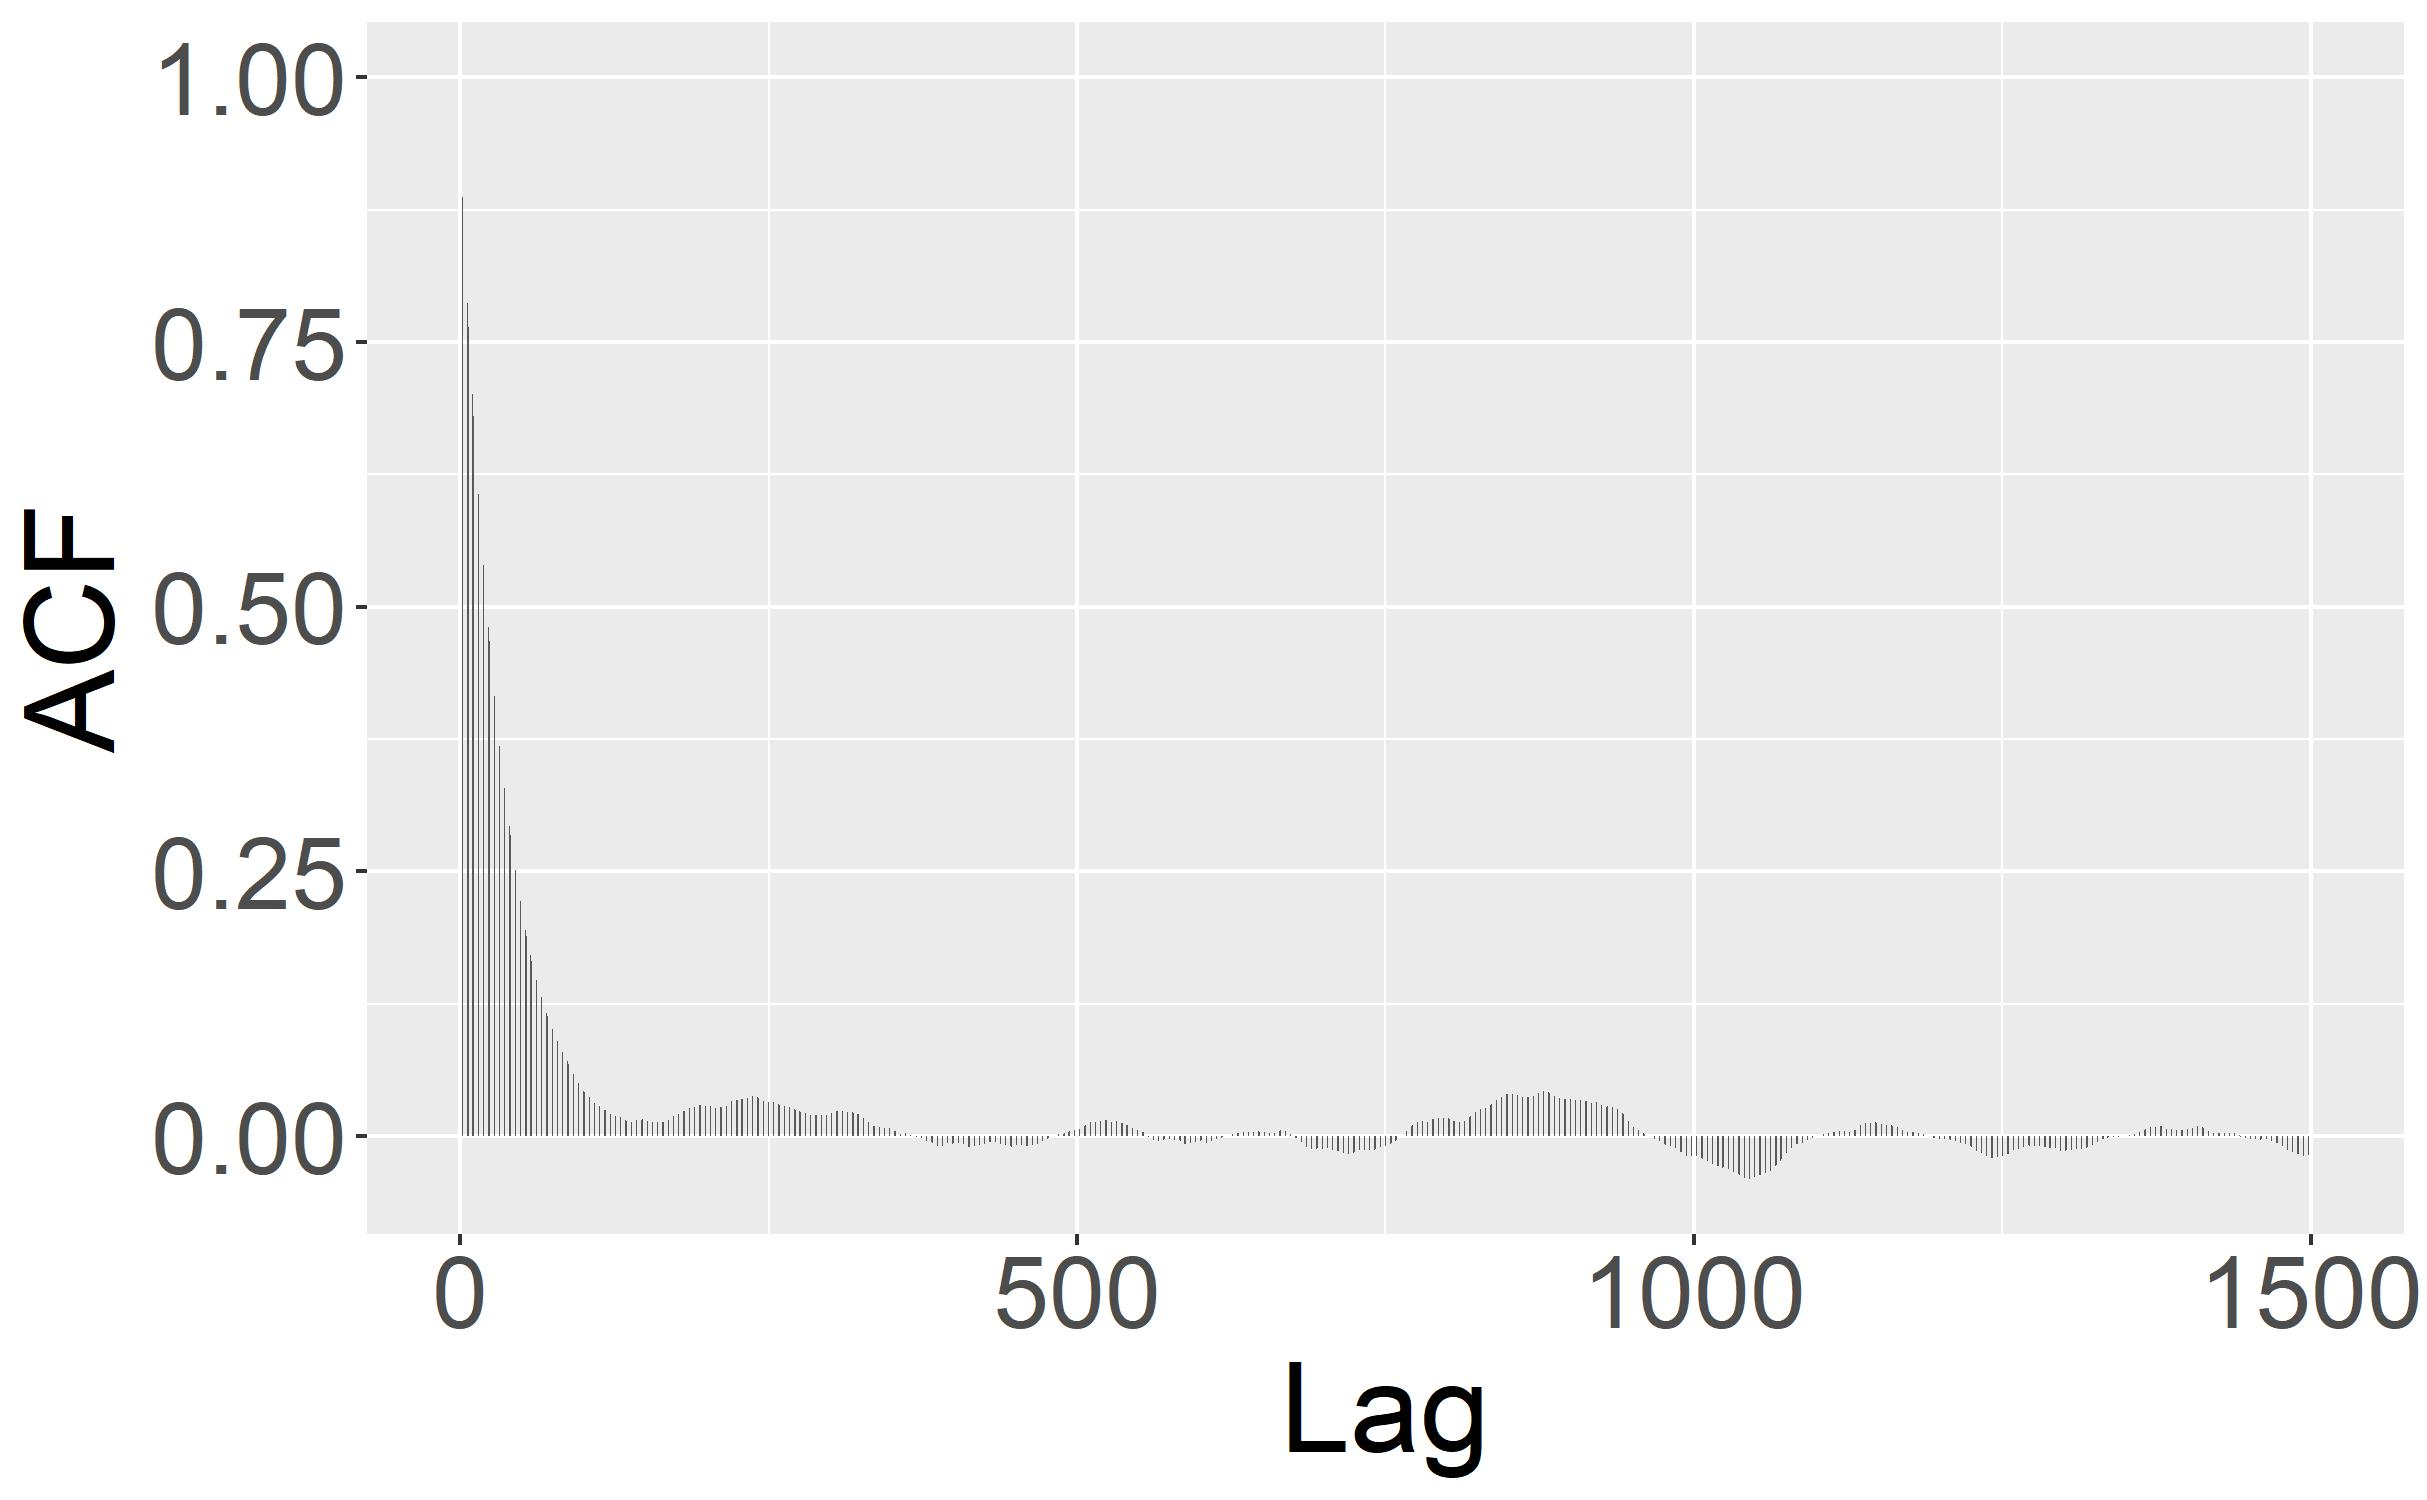
\includegraphics[width=\textwidth]{E1_burn_gamma_acf}
		%	\caption{Auto-correlation function for $\gamma$}
		%	\label{fig:E1_burn_gamma_acf}
		%\end{subfigure}
		\caption{Performance of the DA-MCMC in a medium-sized population for the parameter $\gamma$.}
		\label{fig:E1}
	\end{figure}
	
	The algorithm takes less than $30$ minutes to run $1$ million iterations on a personal laptop. 
	Figure \ref{fig:E1_short_no_burn_gamma_tp} shows the traceplot of the parameter $\gamma$ for the first $10000$ iterations. We observe that the Markov chain quickly migrates from the low density region where it is initialized to the mode of the target distribution. The traceplot of $\gamma$ after a burn-in period of $10000$ iterations in Figure \ref{fig:E1_burn_gamma_tp} indicates that once the chain reaches the high density region it mixes well. The acceptance rate of the MH step is $0.21$.
	The posterior means of $\beta$, $\gamma$ and $R_0$ are respectively $0.00217$, $0.815$ and $2.75$, respectively based on $398$, $370$ and $438$ effective sample sizes. The $90\%$ equal-tailed Bayesian credible intervals are $(0.00166, 0.00278)$, $(0.492, 1.19)$ and $(2.26, 3.45)$ and cover the true values of the parameters. 
	
	We now validate the estimation and uncertainty quantification of the posteriors under our algorithm over repeated simulations. To this end, we examine the frequentist coverage properties of the $90\%$ equal-tailed Bayesian credible interval (BCI). We repeat the previous simulation $2000$ times and compute the posterior mean of the parameters and the corresponding credible intervals. Since the prior is only weakly informative, the observed coverage rate of the BCI should be close to $90\%$.
	Table \ref{tab:coverage} provides the empirical coverage rate of the BCIs for the parameters $\beta$, $\gamma$ and $R_0$ along with the average and variance of the posterior means. As expected, the credible intervals cover the true values around $90\%$ of the time, well within Monte Carlo error of the nominal coverage under a weakly informative prior. This result suggests that running the Markov chain for $1$ million iterations is sufficient to approximate the posterior distribution of the parameters.
	
    \begin{table}
    \centering
    \begin{tabular}{ C{2cm}| *{3}{C{3cm}}}
        %\hline
        Parameter & Observed coverage rate & Average of the posterior means & SD of the posterior means \\ 
        \hline
        $\beta$ & 0.895 & 0.0025 & 0.000255 \\ 
        $\gamma$ & 0.902 & 1.00 & 0.142 \\ 
        $R_0$ & 0.910 & 2.54 & 0.194 \\
        \hline
    \end{tabular}
    \caption{Empirical coverage of the $90\%$ posterior credible intervals and distribution of the posterior means from $2000$ independent runs in a medium-sized population ($n=1000$). The true values of the parameters are $(\beta, \gamma, R_0) = (0.0025, 1, 2.5)$. The standard errors for the observed coverage rate are calculated as $\sqrt{\hat{p}(1-\hat{p})/2000}$, which results in a largest standard error of $6.8$e-3.}
    \label{tab:coverage}
    \end{table}
	
	Second, we explore the impact of the tuning parameter $\rho$ on the mixing properties of the algorithm as the population size varies.
	We simulate three realizations from the SIR process with $S(0) \in \{250, 500, 1000\}$ with  $I(0)=10$, $\gamma=1$, $t_{end} = 6$ and $K = 10$ for each simulation. We choose $\beta$ so that $R_0 \in \{3, 2.5, 2\}$ respectively, in order to have epidemics with comparable dynamics. For each population size and each value $\rho \in \{0.02, 0.05, 0.1, 0.25, 0.5, 1\}$, the DA-MCMC algorithm is run for $1$ million iterations. We use the effective sample size per second to compare the resulting Markov chains.
	
	Figures \ref{fig:E3_runtime} and \ref{fig:E3_accept} show the run time of the algorithm and the acceptance rate in the MH step. We observe that, as expecetd, the run time increases with the population size and with $\rho$, which reflects the fact that the number of random variables to generate per iteration is proportional to $\lceil\rho n\rceil$. Moreover, the acceptance rate decreases as the number of trajectories updated per iteration $\lceil\rho n\rceil$ increases.
	Finally, the effect of $\rho$ on the mixing properties of the Markov chain is presented in Figure \ref{fig:E3_facet_ESSsecR0}. We observe that for a population of $250$ individuals updating the entire latent data in the MH step provides the best mixing; as the population size increases, however, the optimal value of $\rho$ decreases. For instance, this suggests that, for a population of $1000$ individuals, updating the whole latent data results in an excessively low acceptance rate, while updating less than $10$\% makes the updates too small to efficiently explore the latent space.
	
	\begin{figure}
		\centering
		\begin{subfigure}[b]{0.32\textwidth}
			\centering
			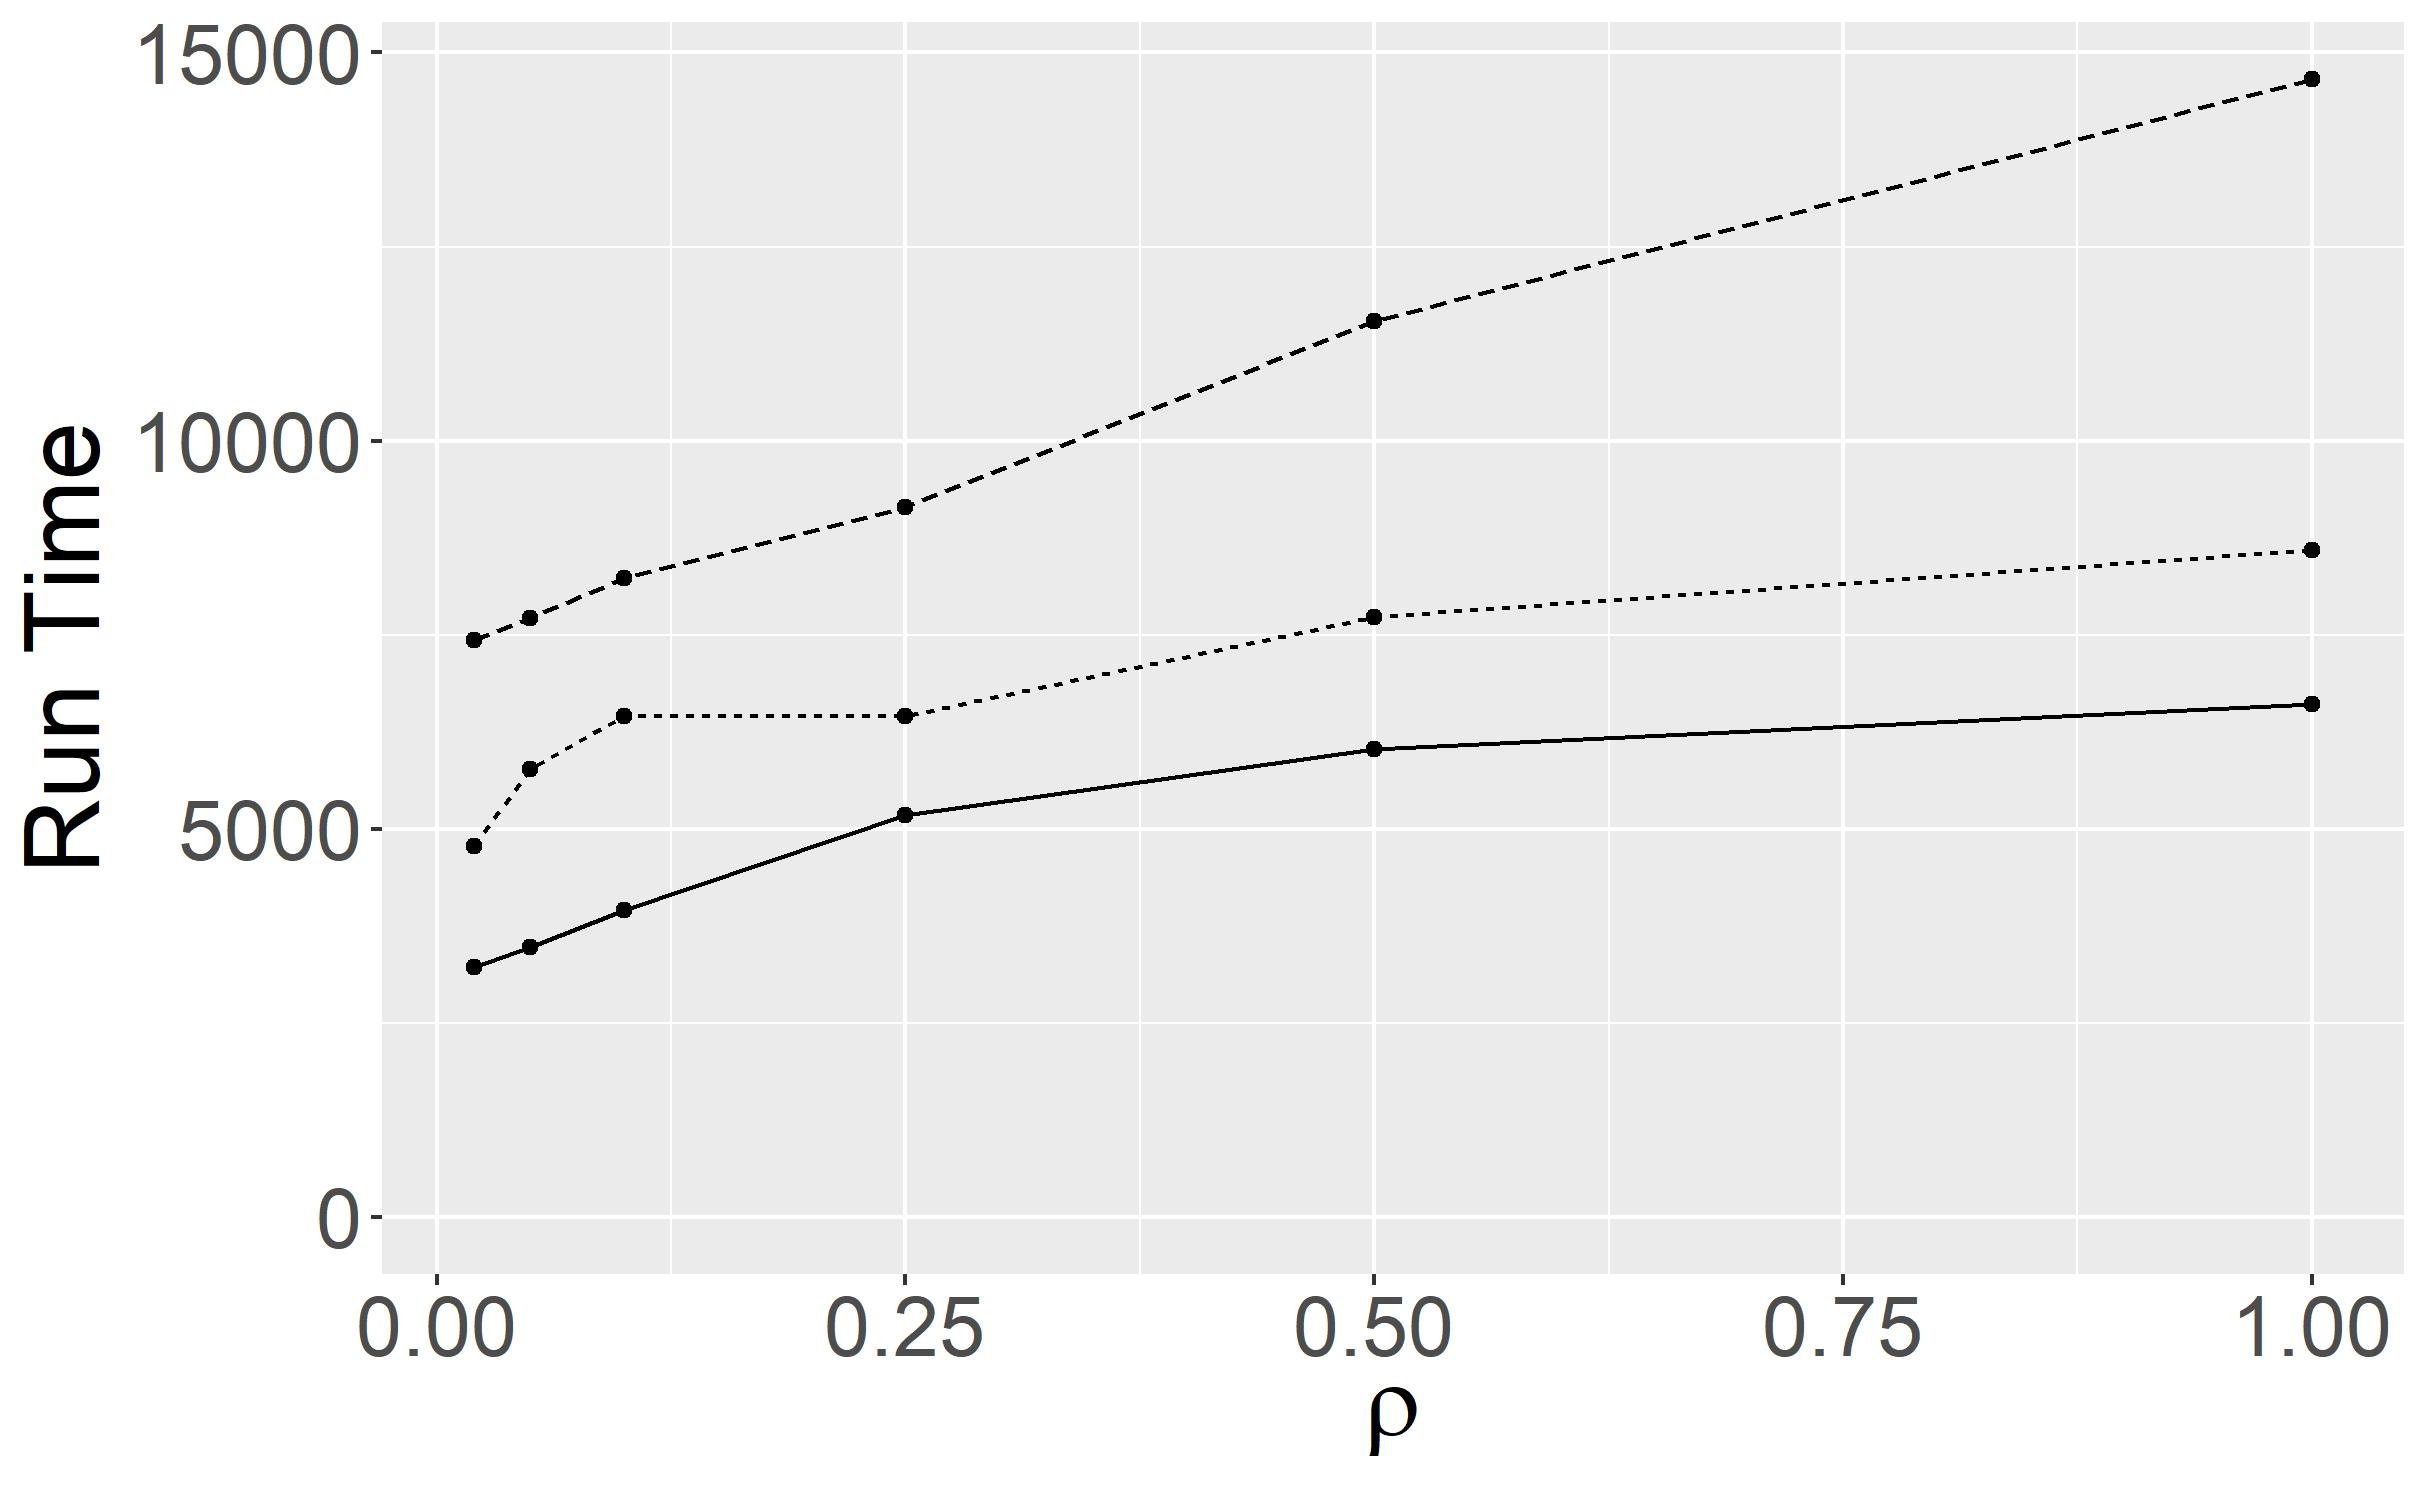
\includegraphics[width=\textwidth]{E3_runtime}
			\caption{Run time in minutes}
			\label{fig:E3_runtime}
		\end{subfigure}
		\hfill
		\begin{subfigure}[b]{0.32\textwidth}
			\centering
			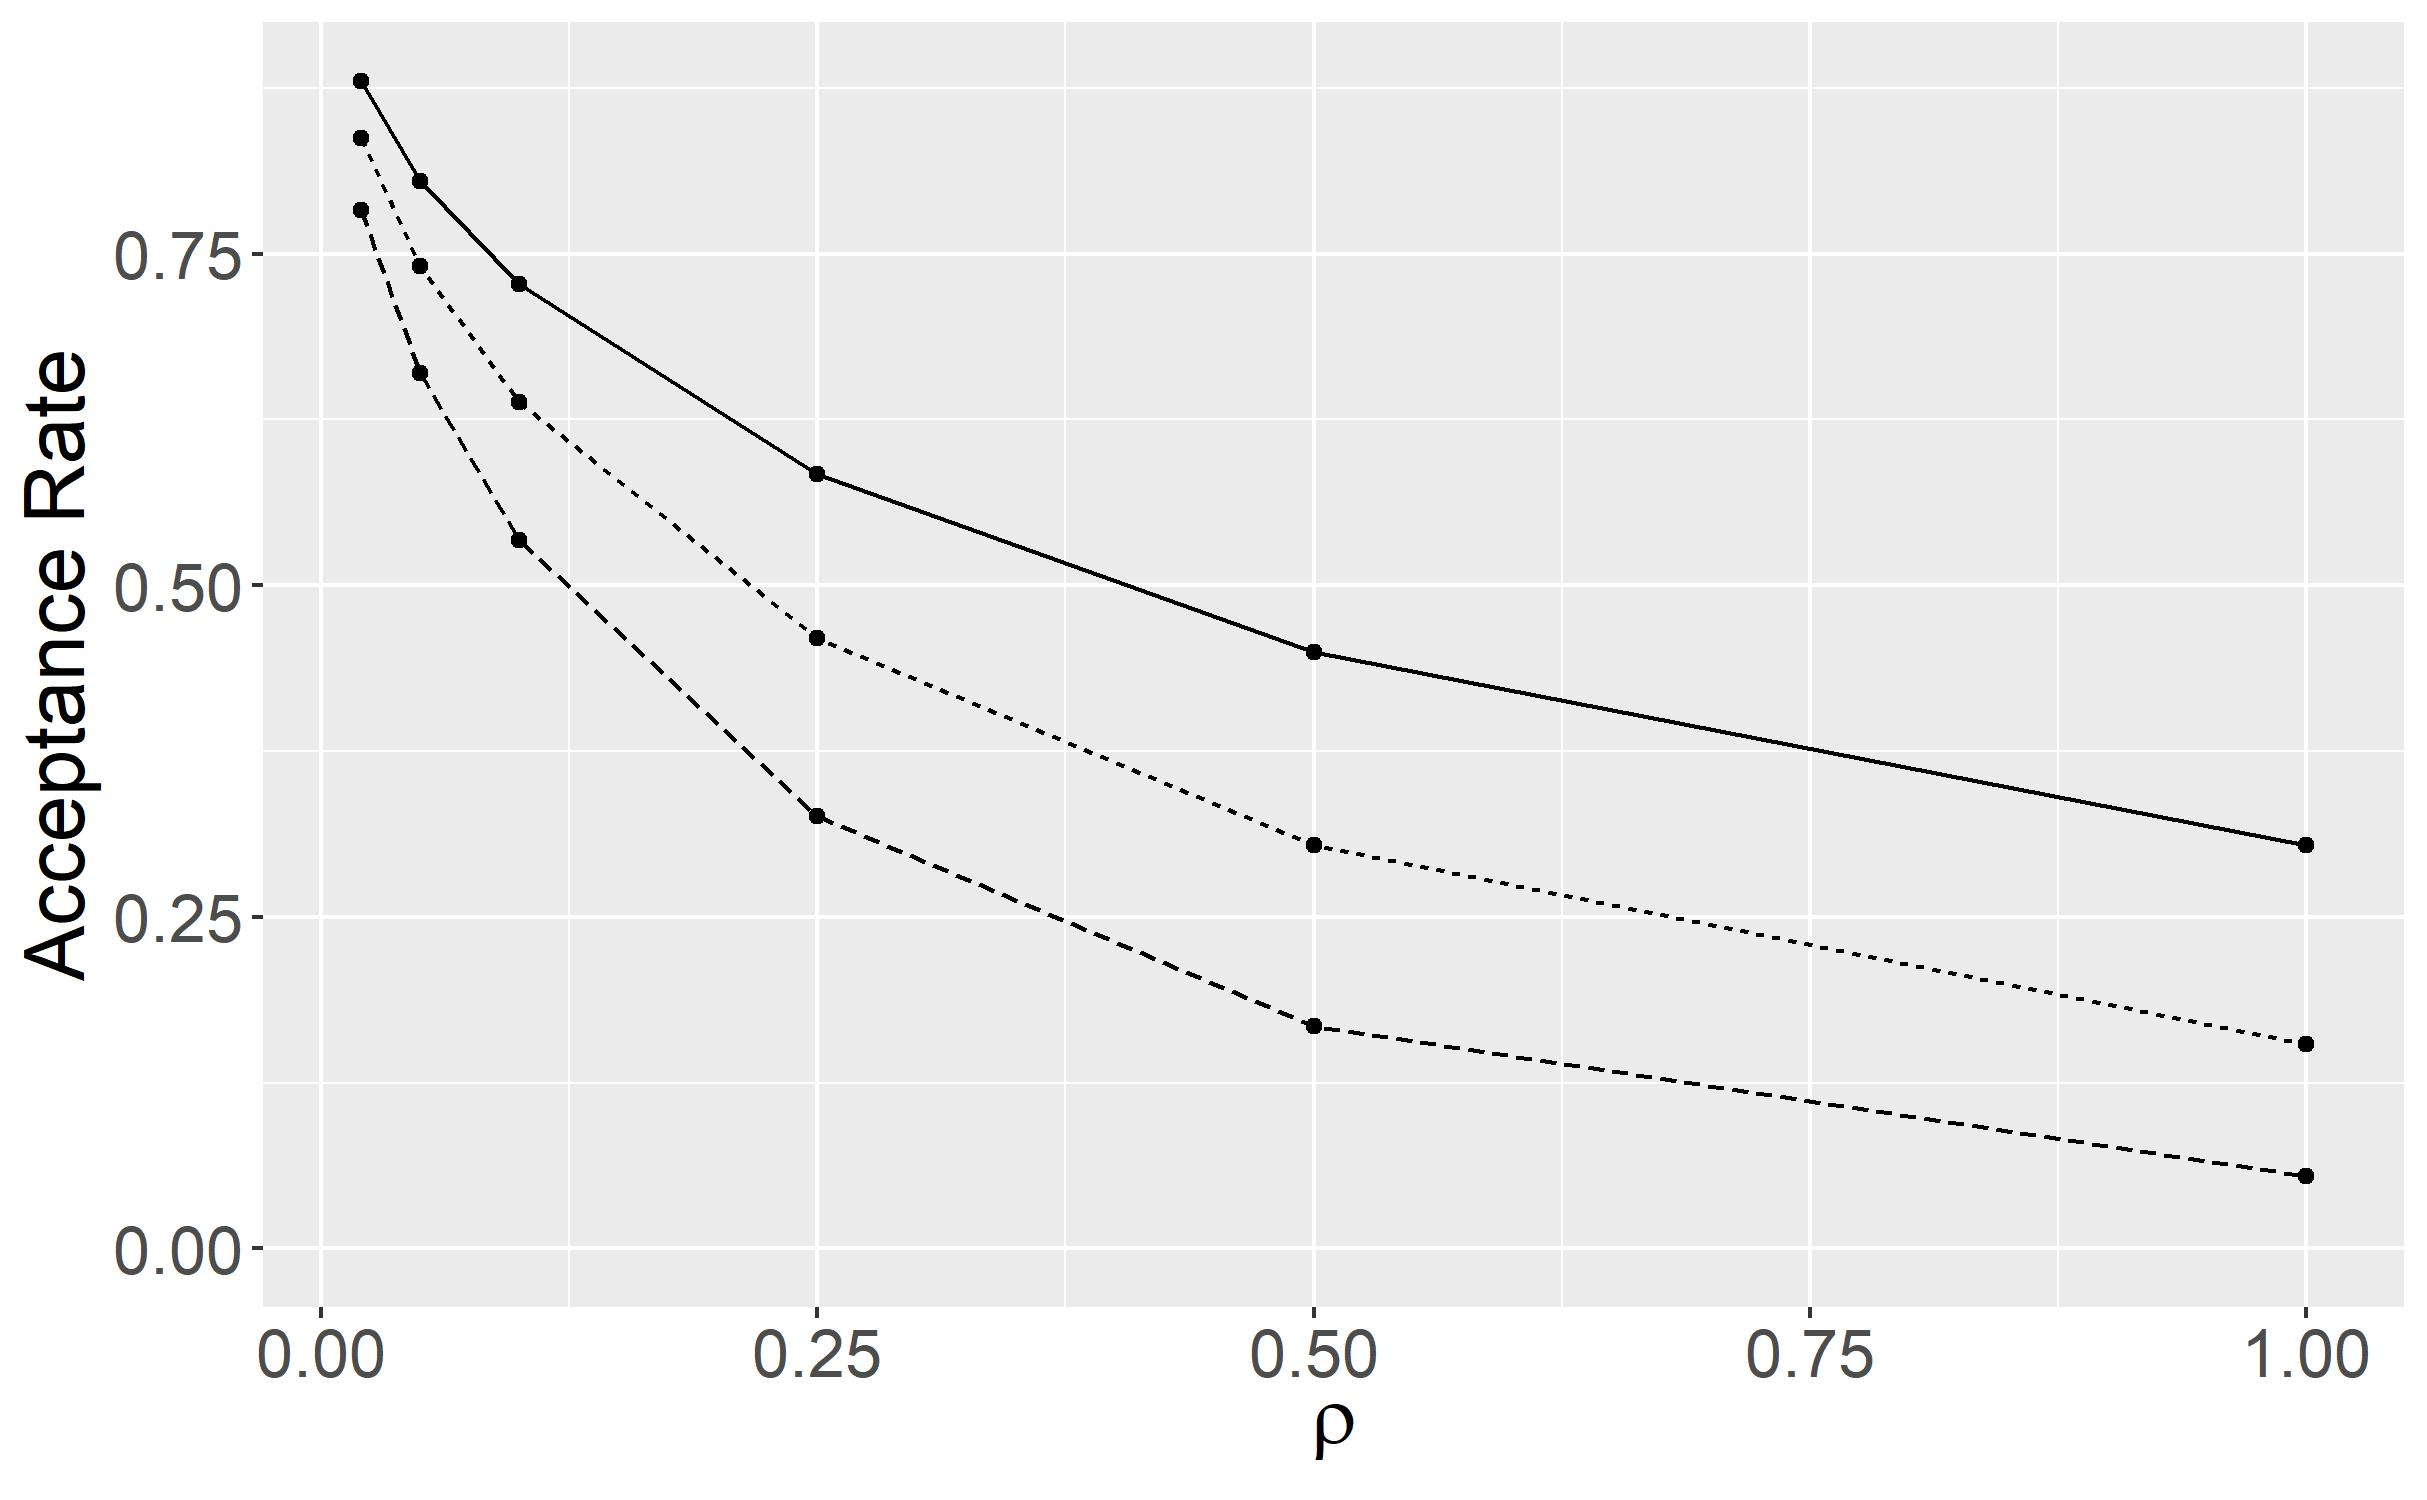
\includegraphics[width=\textwidth]{E3_accept}
			\caption{Acceptance rate}
			\label{fig:E3_accept}
		\end{subfigure}
		\hfill
		\begin{subfigure}[b]{0.32\textwidth}
			\centering
			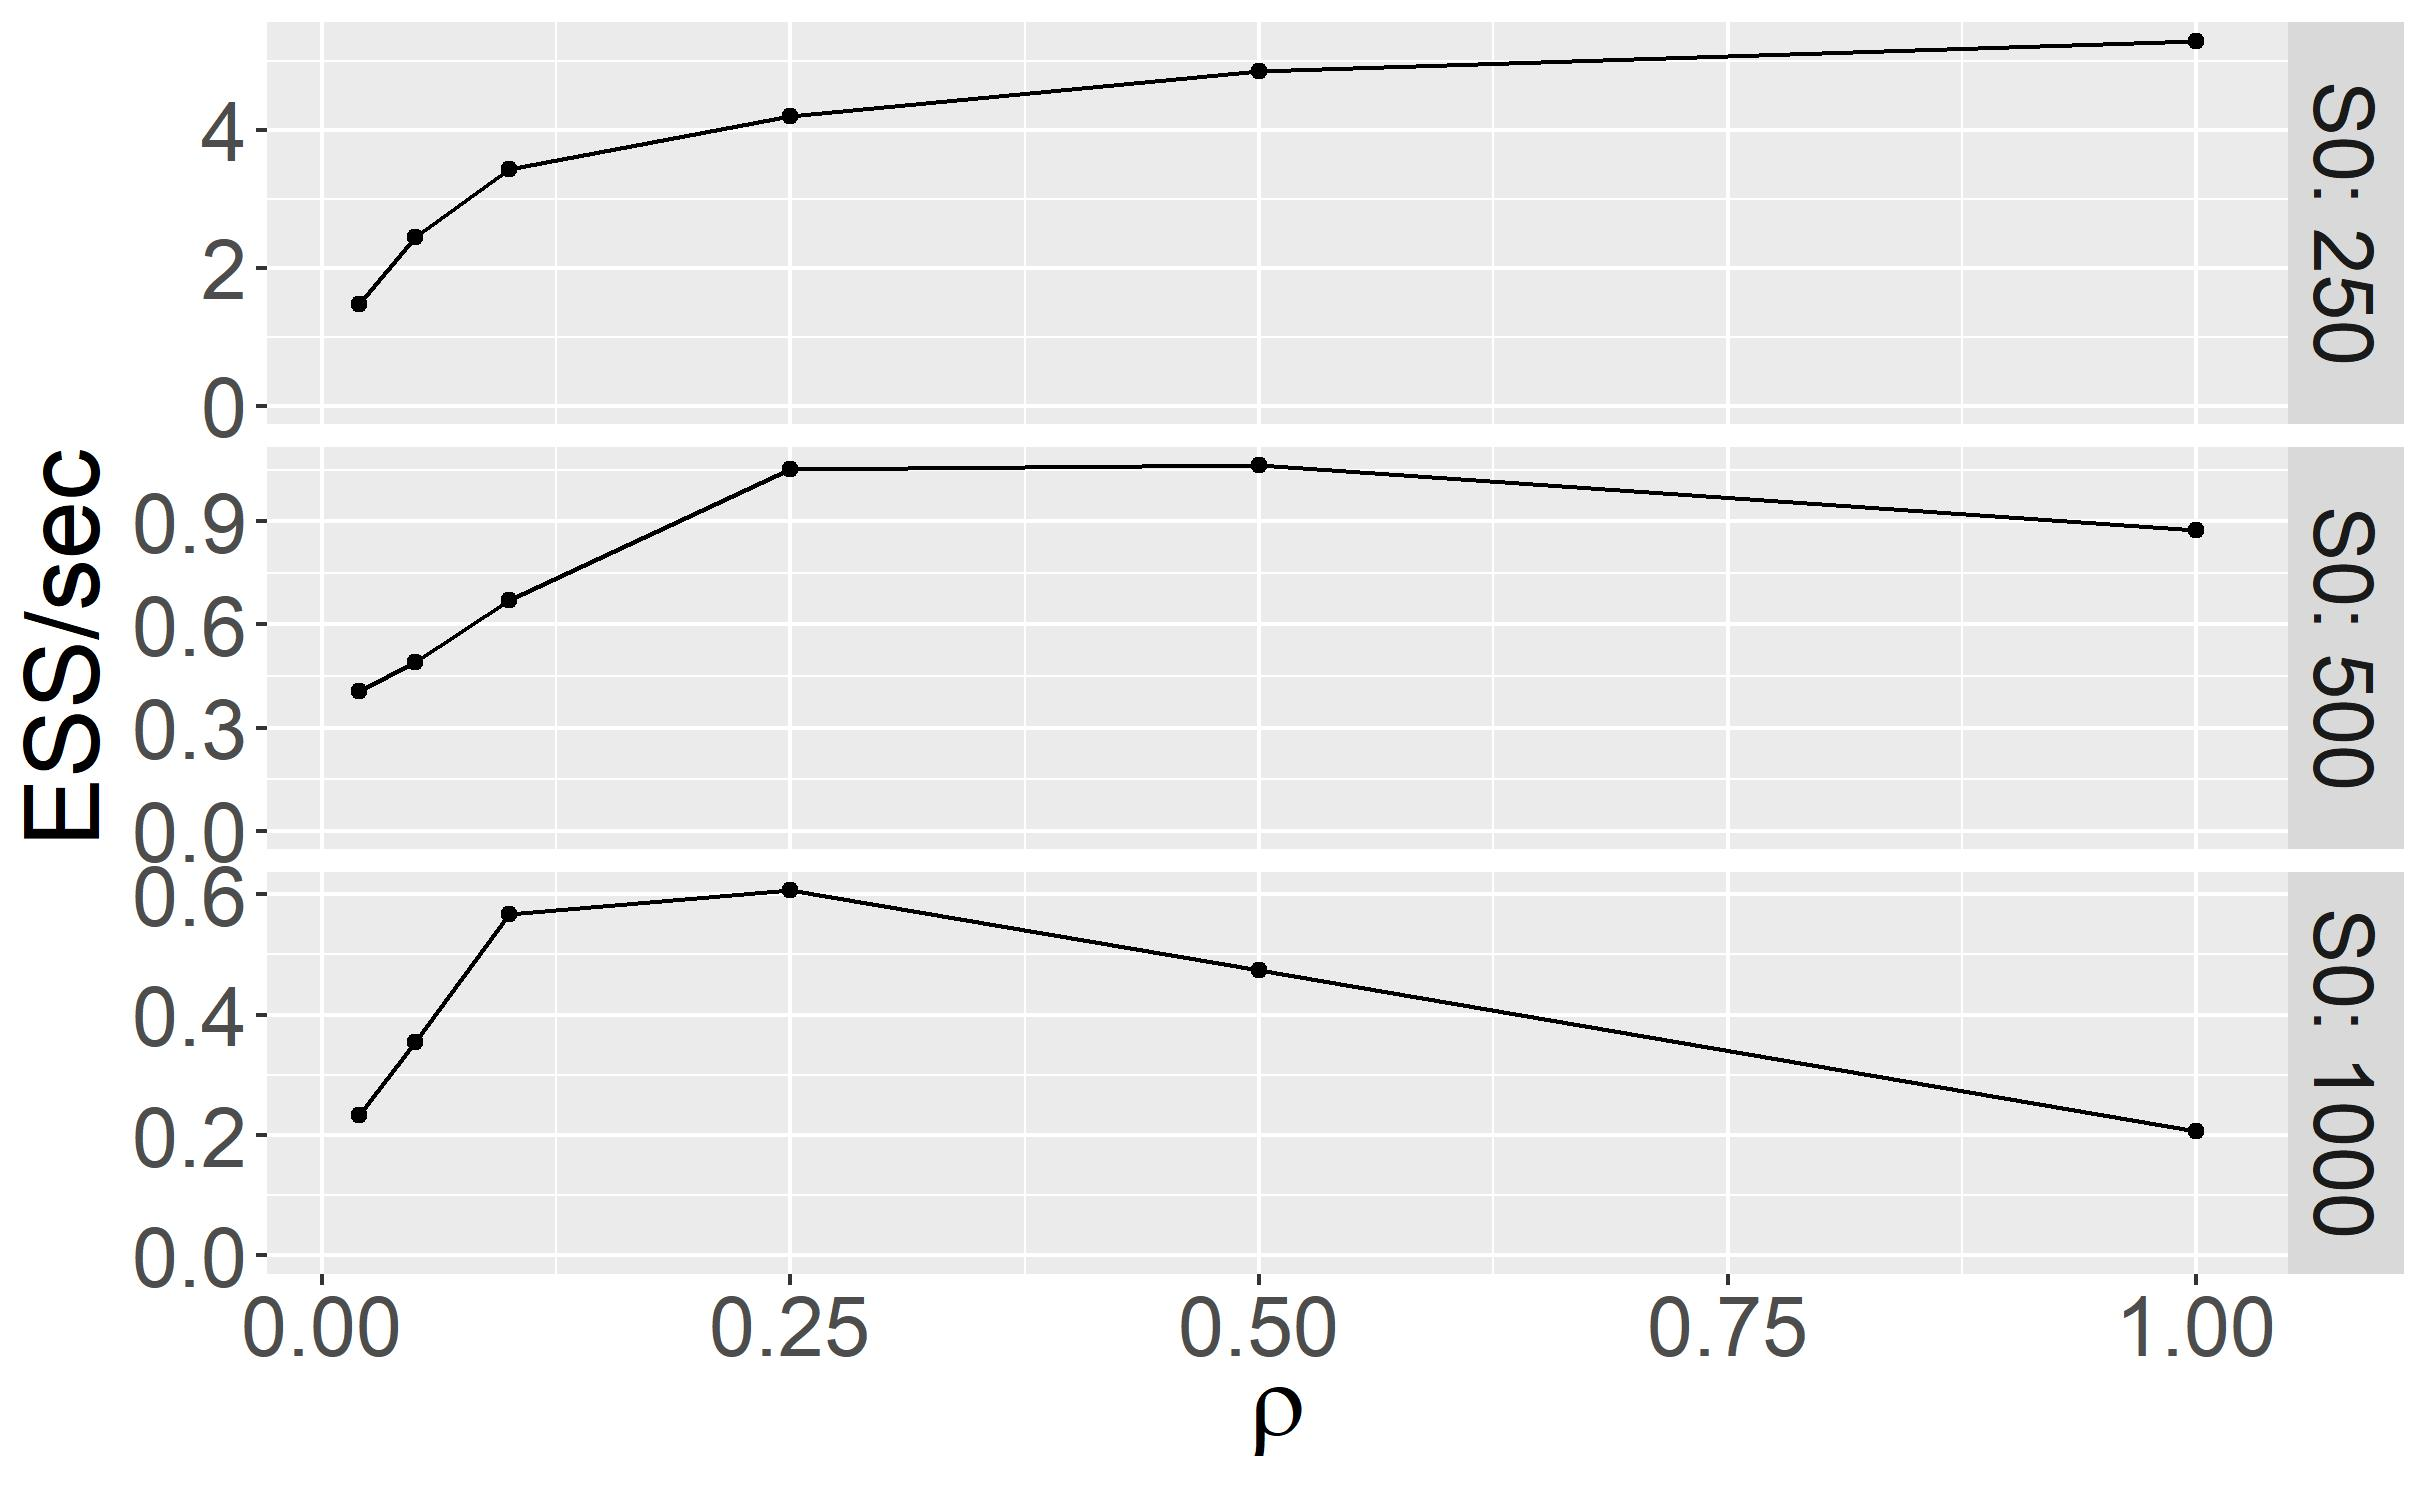
\includegraphics[width=\textwidth]{E3_facet_ESSsecR0}
			\caption{ESS/sec for $R_0$
			%Acceptance rate of the proposed latent spaces in the Metropolis-Hastings step of the MCMC algorithm across different population sizes and values for $\rho$.
			}
			\label{fig:E3_facet_ESSsecR0}
		\end{subfigure}
		\caption{Impact of $\rho$ on the performance of the DA-MCMC in a population of size $250$ (solid), $500$ (dotted) and $1000$ (dashed).}
		\label{fig:E3}
	\end{figure}
		
	Finally, we showcase the efficacy of our joint proposal scheme through a comparison %the performance of the proposed DA-MCMC algorithm in which event times are jointly proposed 
	to a SSU DA-MCMC that is similar in spirit to those in \cite{Gibson.1998, ONeill.1999, Fintzi.2017}. We do not consider particle filters \cite{King.2015} nor diffusion approximations \cite{Fintzi.2020} since these methods are not suited to situations in which the counts are observed without error.
	The SSU sampler that we consider here is a special case of our DA-MCMC in which $\rho = (S(0)+I(0))^{-1}$, so that the infection and removal times of a single individual are updated per iteration. The two algorithms are run on the same data of a moderately sized population for $1$ million iterations. Figure \ref{fig:E6} presents the traceplots for $\gamma$ as well as the auto-correlation function. We observe that the Markov chain mixes much better when event times are jointly proposed in the MH step. This is supported quantitatively in Table \ref{tab:E6} which shows that the ESS per second obtained with the proposed DA-MCMC is between 7 and 20 times larger than that of the SSU DA-MCMC. Hence, even though the computation cost per iteration is larger for our algorithm, it mixes better than SSU algorithms and is more efficient overall.
	
	\begin{figure}
		\centering
		\begin{subfigure}[b]{0.49\textwidth}
			\centering
			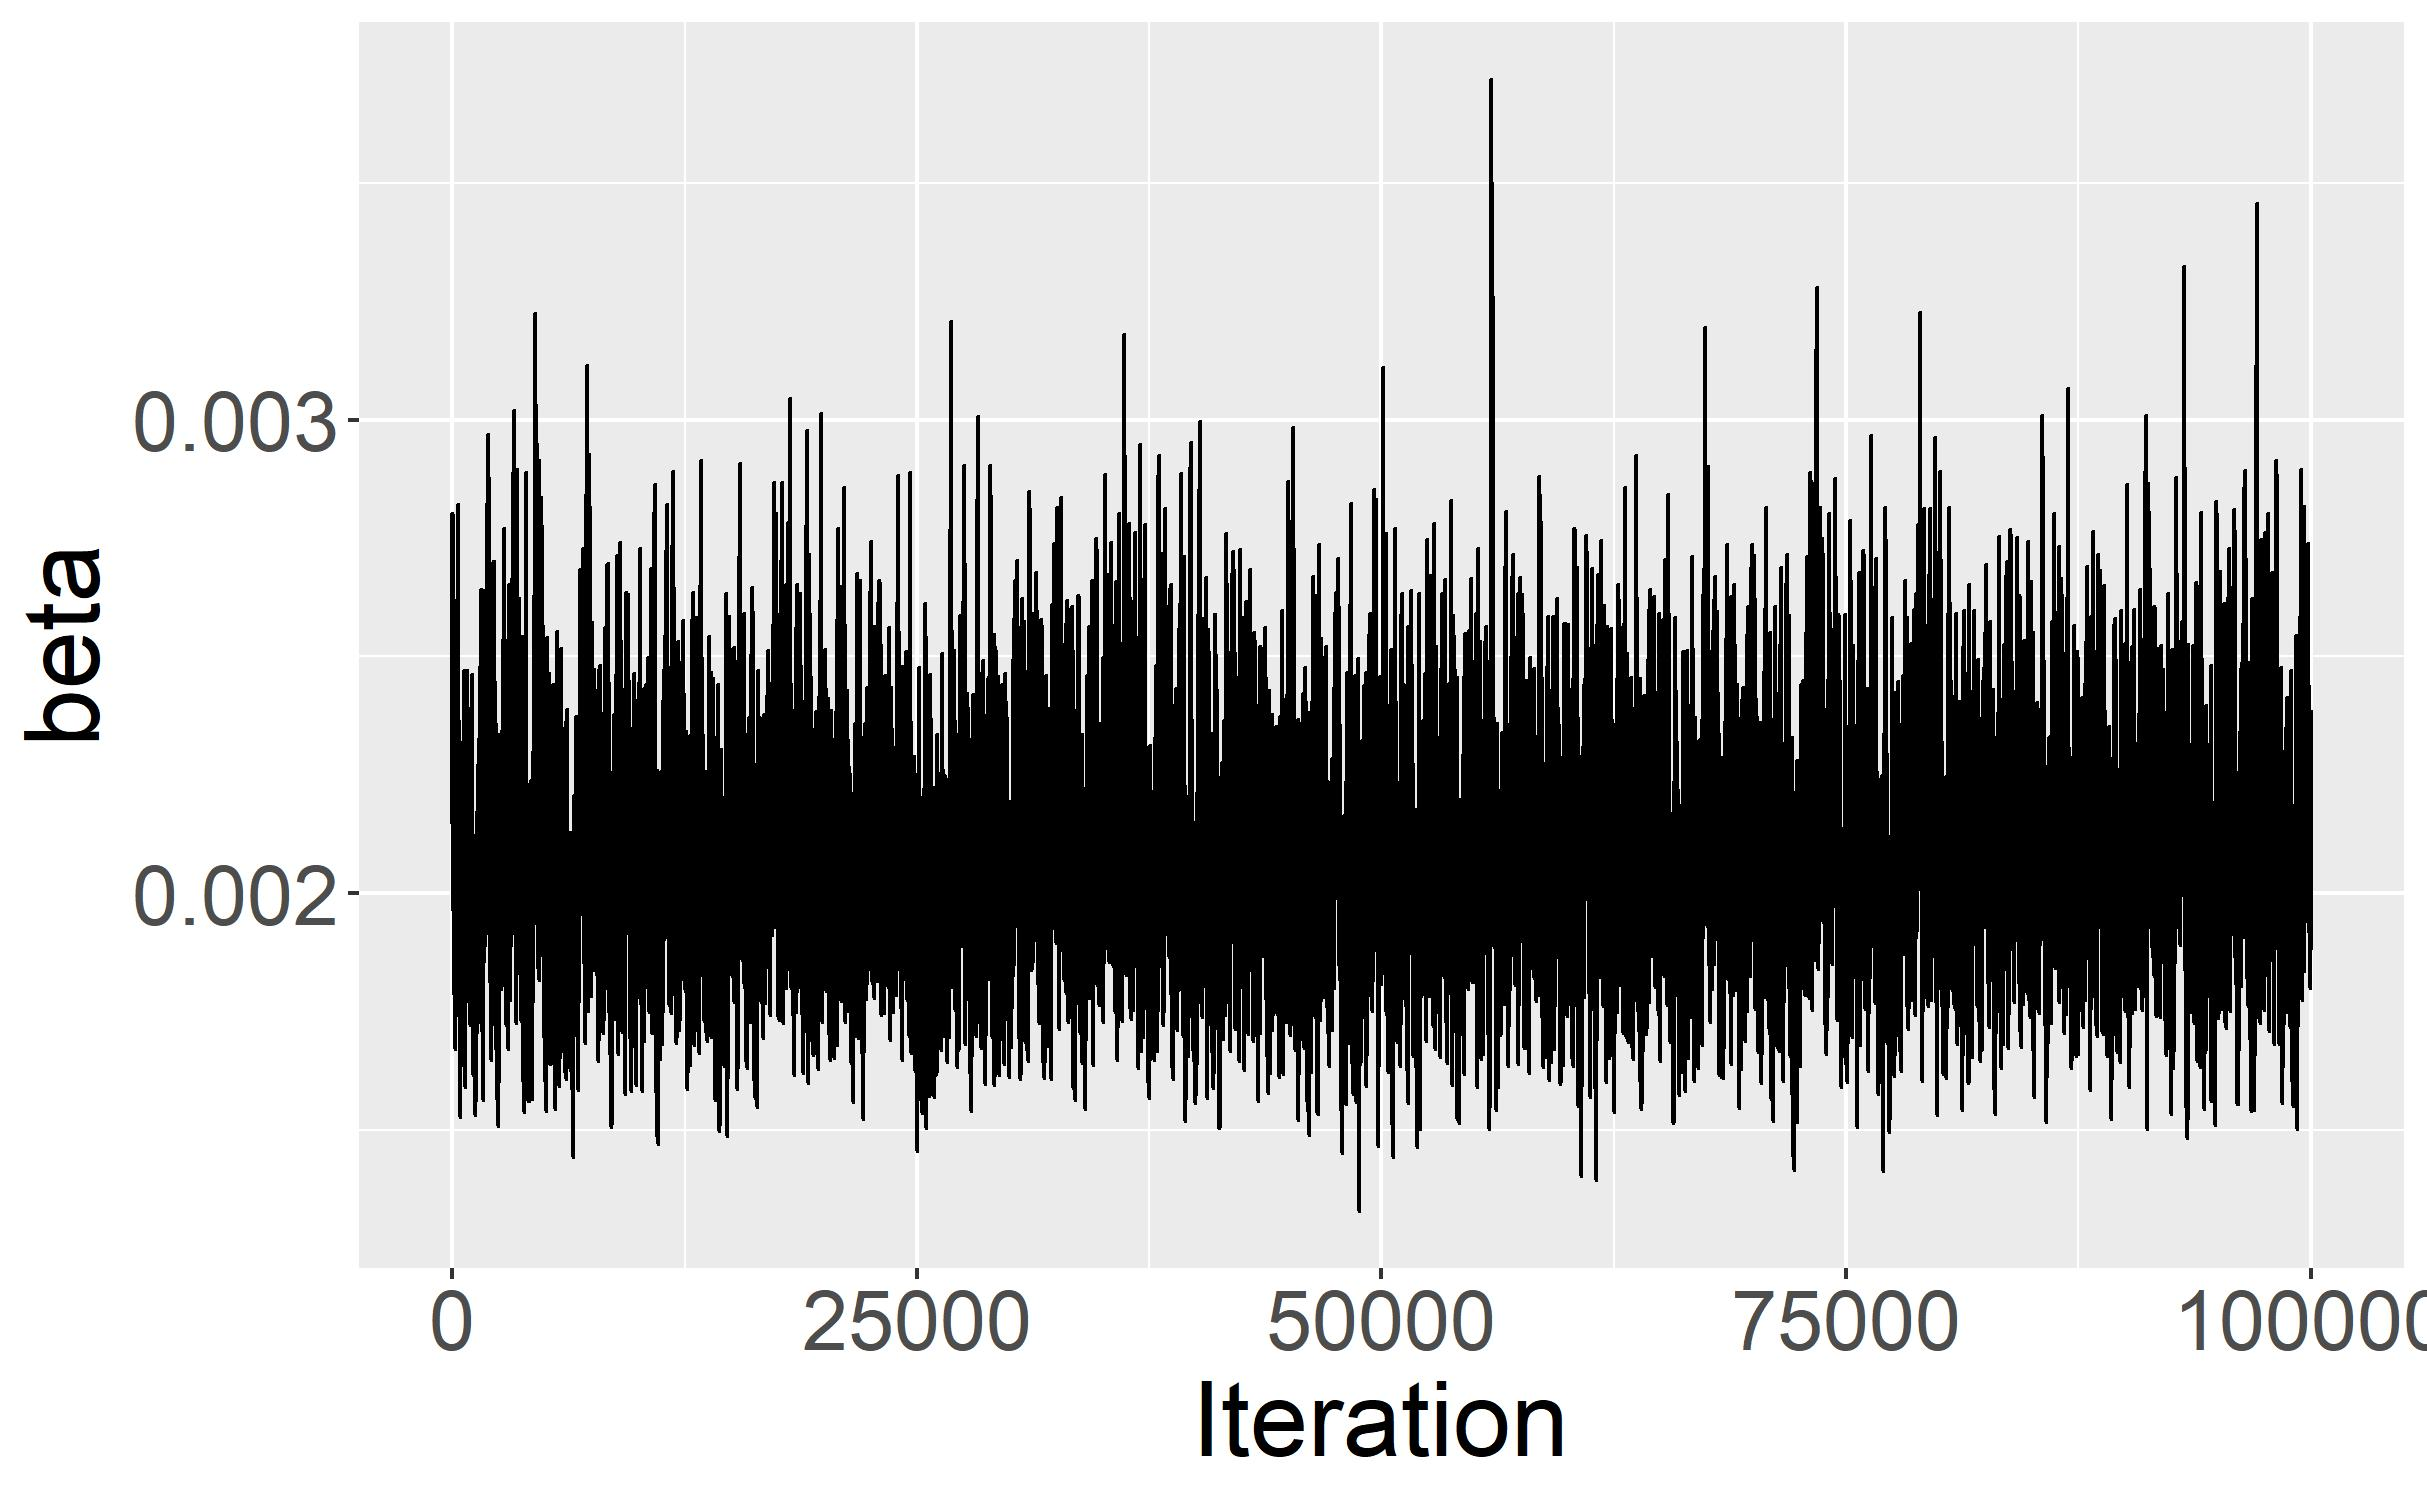
\includegraphics[width=0.49\textwidth]{E6_no_burn_beta_tp_joint.jpg}
			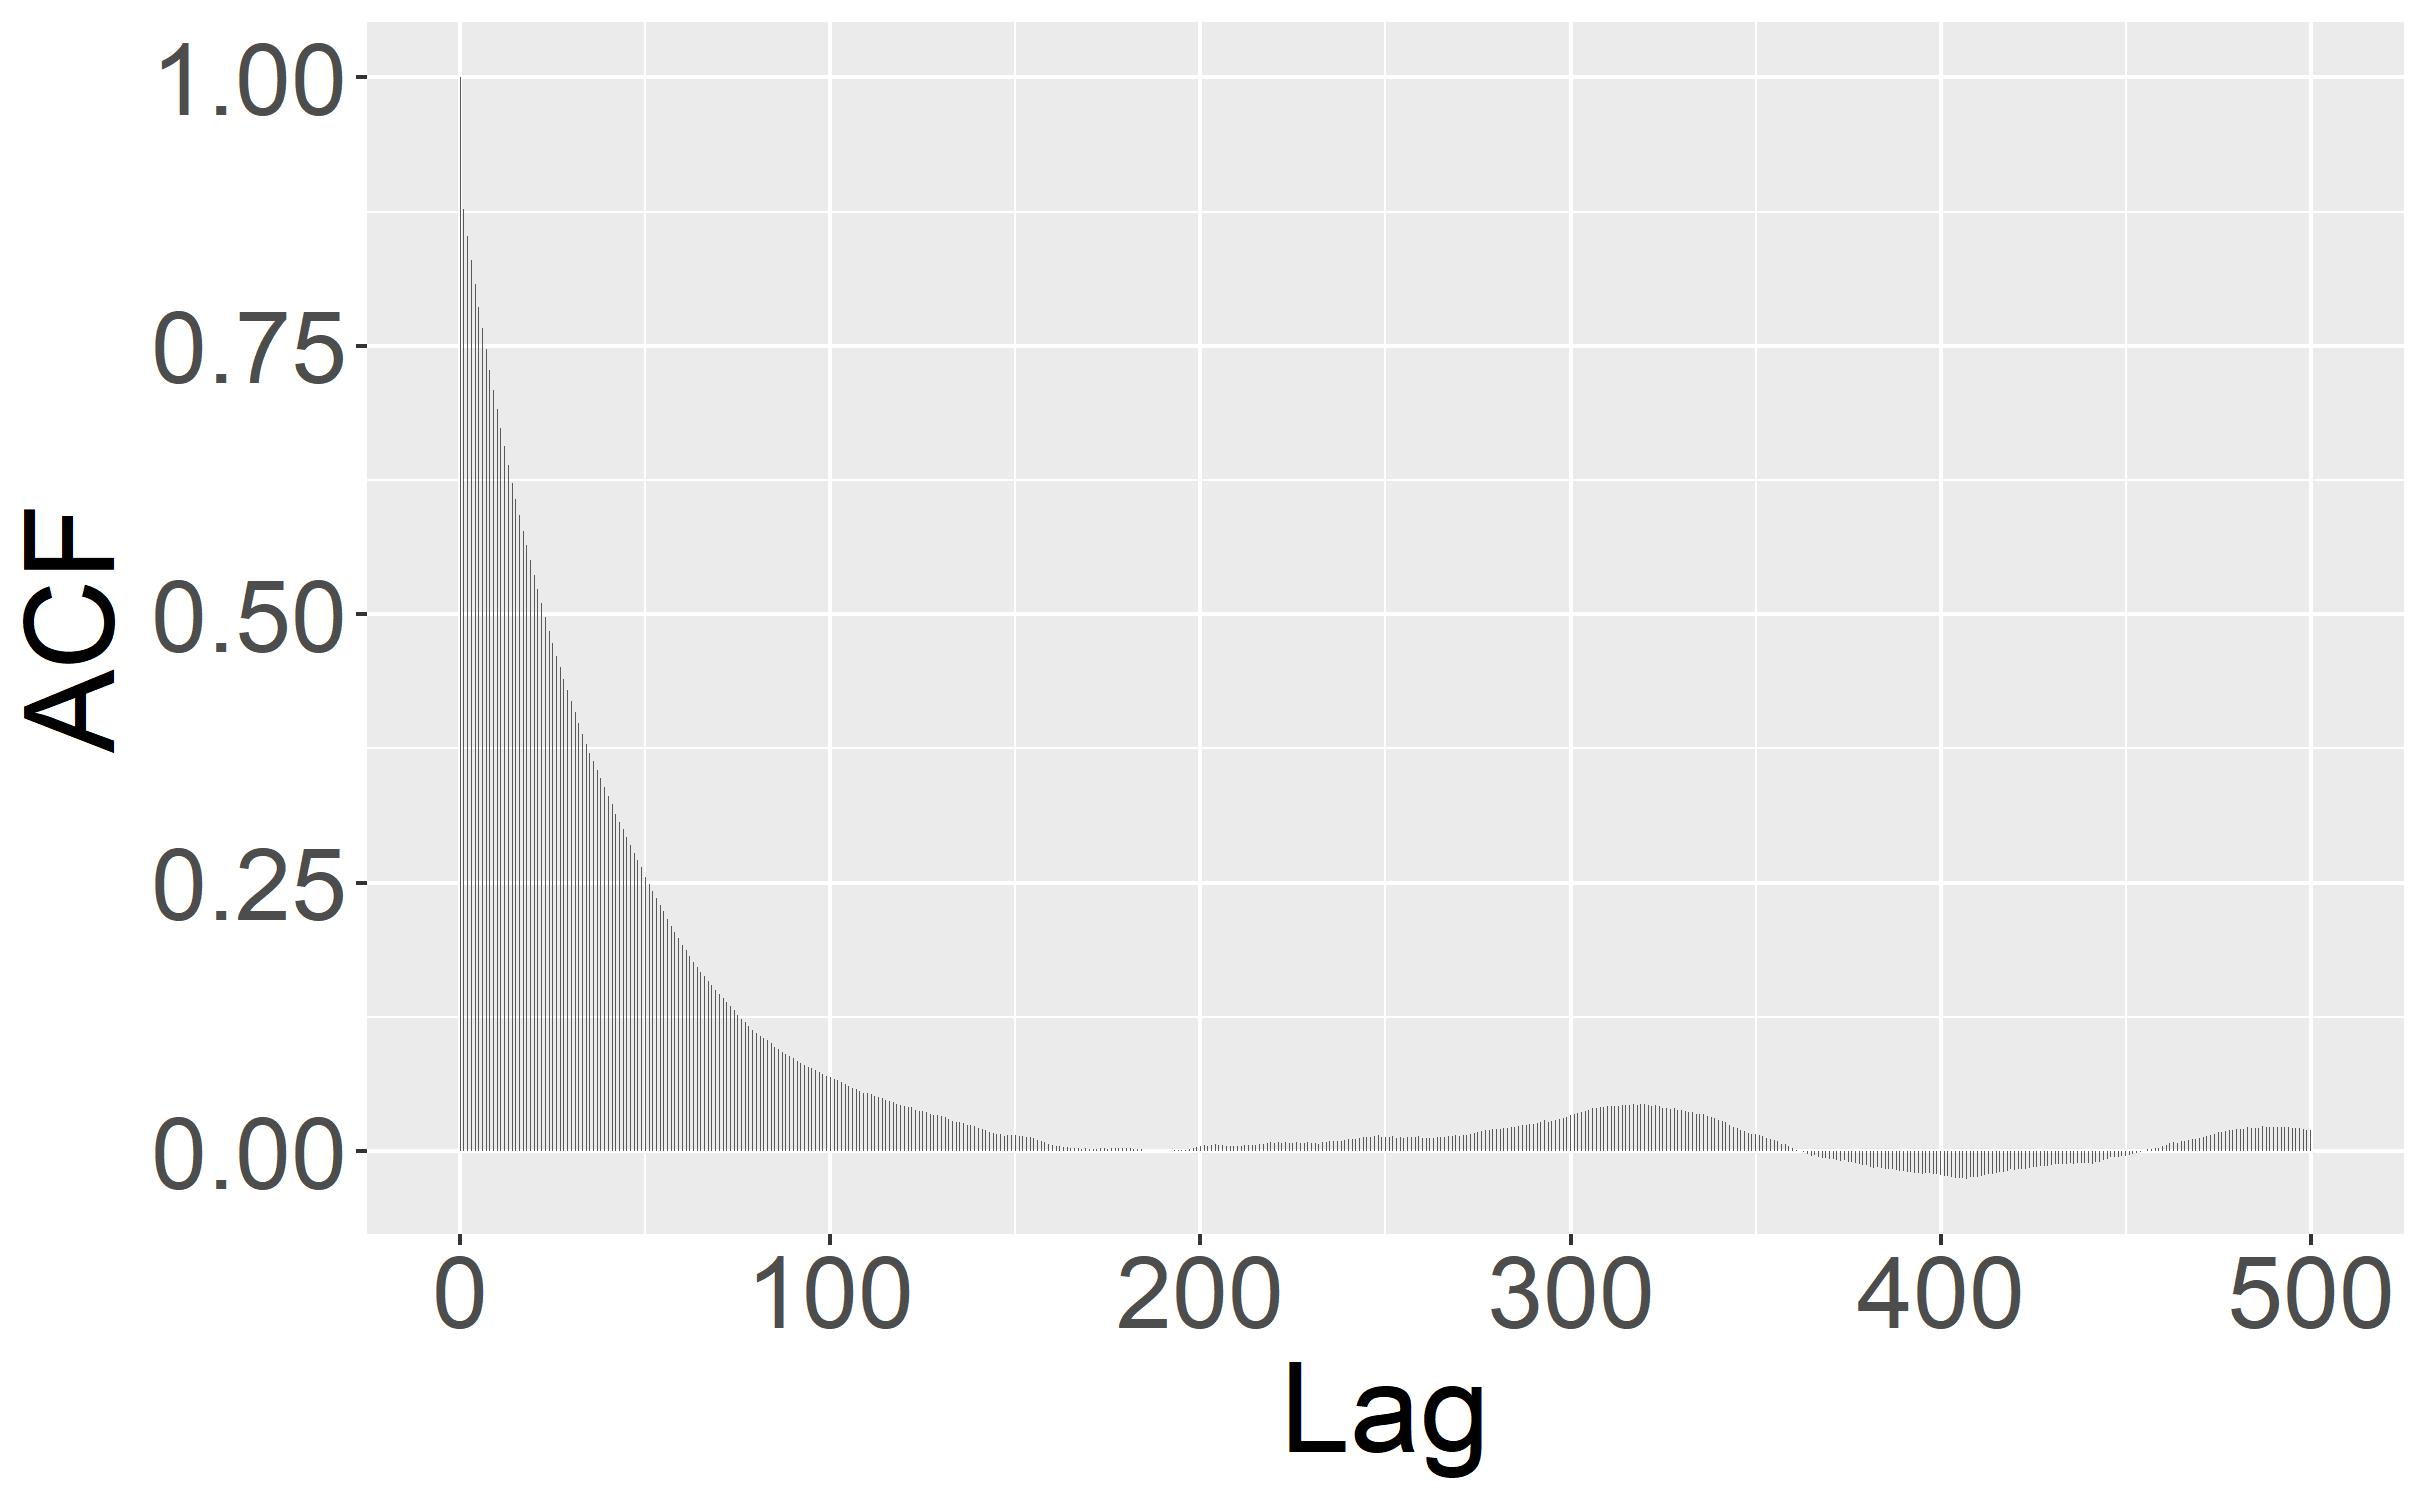
\includegraphics[width=0.49\textwidth]{E6_burn_beta_acf_joint.jpg}
			\caption{DA-MCMC}
			\label{fig:E6_no_burn_beta_tp_joint}
		\end{subfigure}
		\hfill
		\begin{subfigure}[b]{0.49\textwidth}
			\centering
			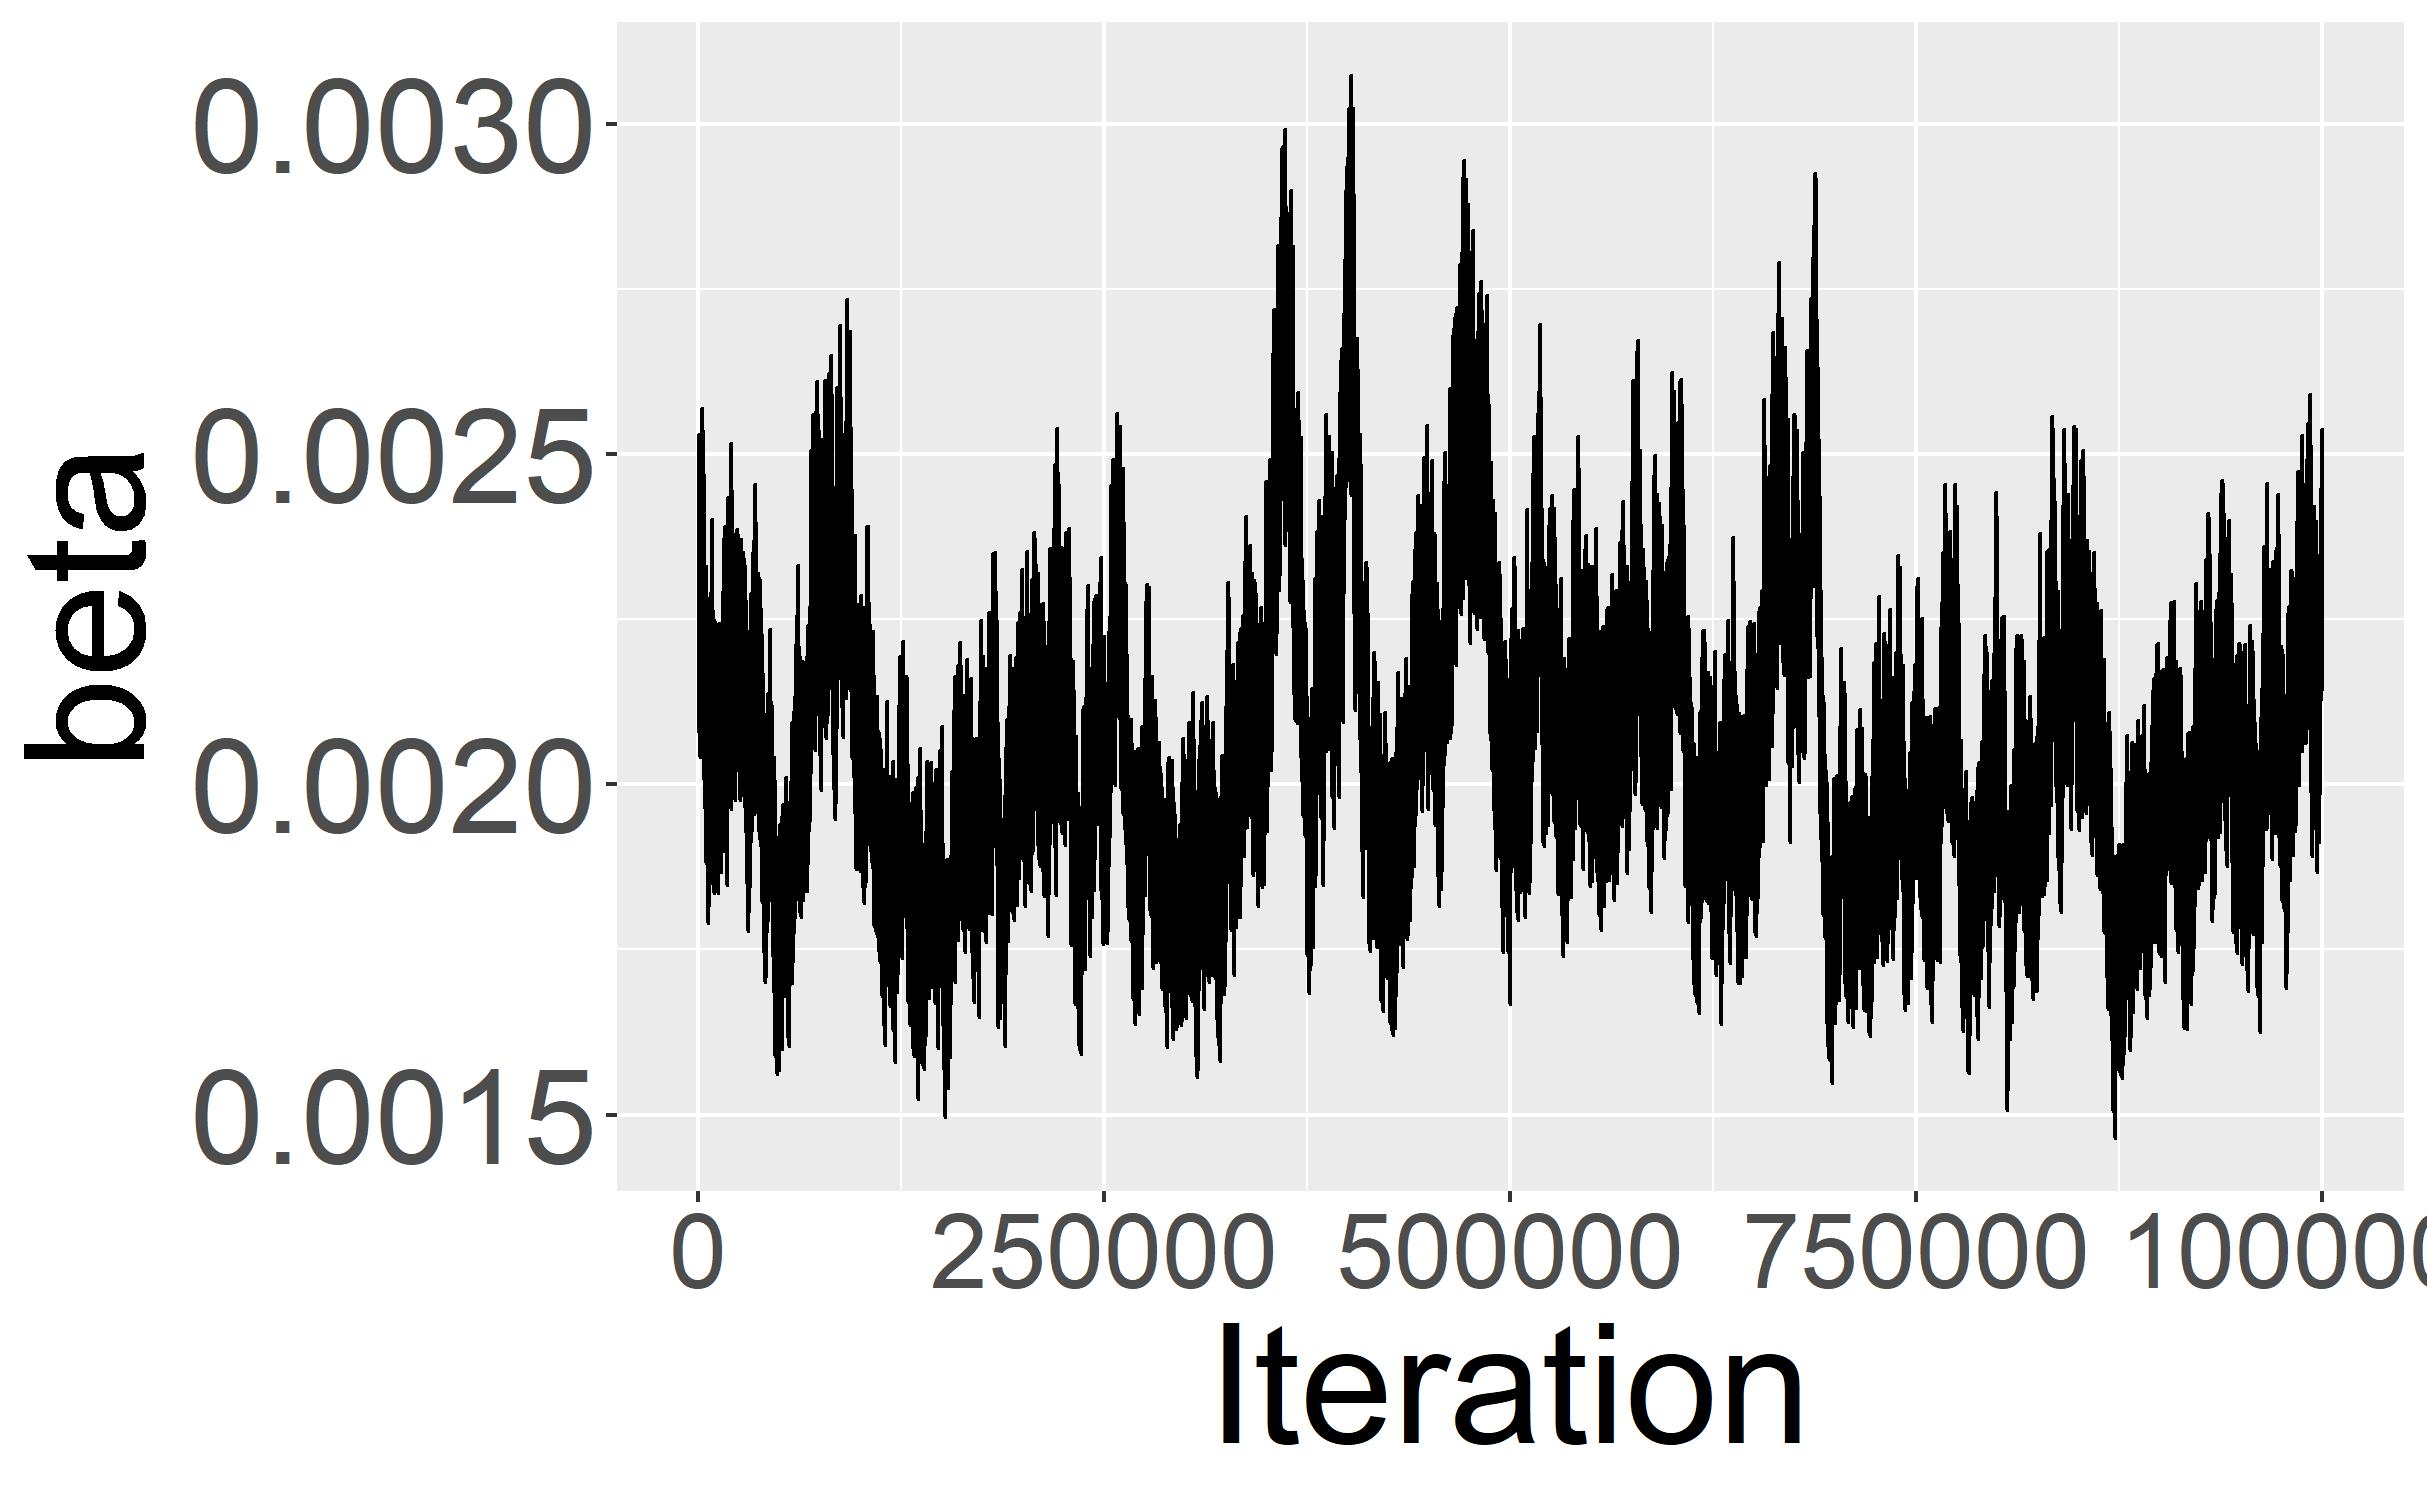
\includegraphics[width=0.49\textwidth]{E6_no_burn_beta_tp_single.jpg}
			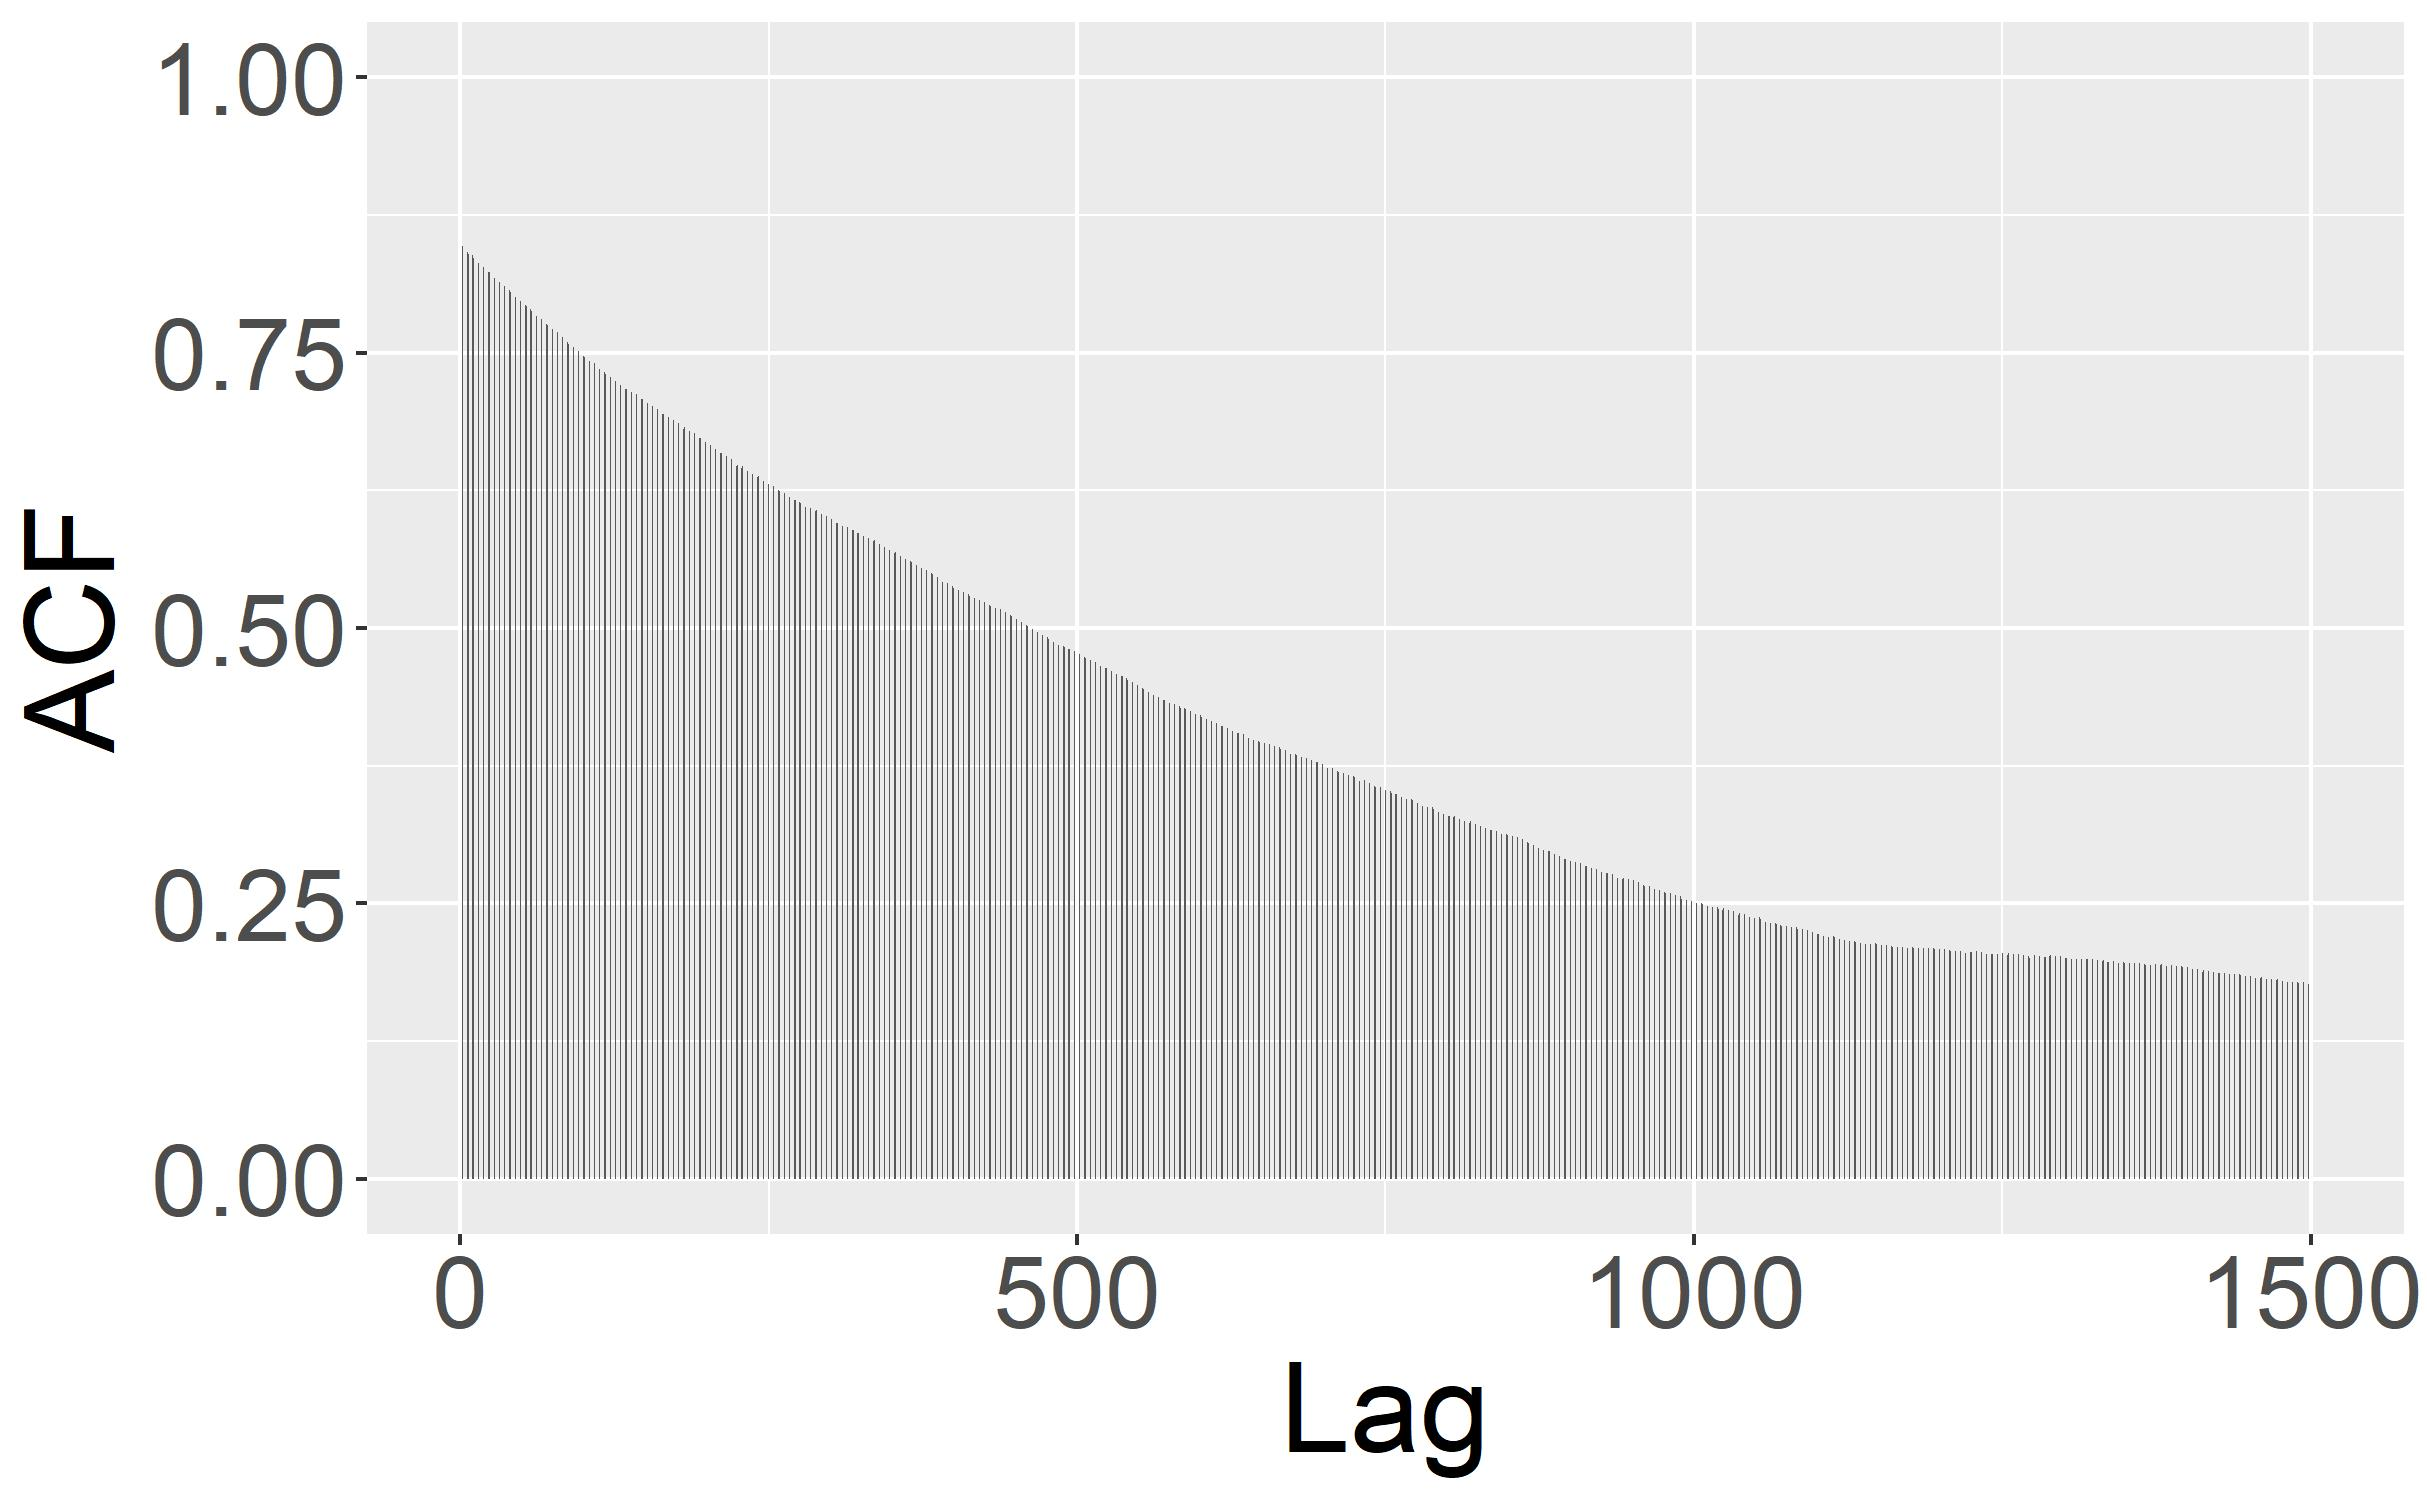
\includegraphics[width=0.49\textwidth]{E6_burn_beta_acf_single.jpg}
			\caption{SSU DA-MCMC}
			\label{fig:E6_no_burn_beta_tp_single}
		\end{subfigure}
		\caption{Traceplots and auto-correlation functions of the proposed DA-MCMC and the SSU DA-MCMC for $\beta$.}
		\label{fig:E6}
	\end{figure}
	
	 \begin{table}
        \centering
        \begin{tabular}{ C{2cm}| *{2}{C{3cm}}}
            Parameter & DA-MCMC & SSU DA-MCMC \\ 
            \hline
            $\beta$ & 0.20 & 0.01 \\ 
            $\gamma$ & 0.19 & 0.01 \\ 
            $R_0$ & 0.38 & 0.05 \\
            \hline
        \end{tabular}
        \caption{Effective sample size per second for the proposed DA-MCMC and the SSU DA-MCMC.}
        \label{tab:E6}
    \end{table}
	
	\subsection{Ebola Outbreak in Gu\'eck\'edou, Guinea}
	\label{sec:ebo}
	%Outline: background; setup; results; table; figure
	
	We now turn to a case study concerning the 2013-2015 Ebola outbreak in Western Africa.
	Between late $2013$ and $2015$, Guinea, along with several neighboring countries, experienced the largest outbreak of the Ebola virus disease in history. The virus, which has a fatality rate of $70\%$, was responsible for the death of almost $2000$ people in Guinea alone.
	The outbreak is believed to have originated in the Gu\'eck\'edou prefecture of Guinea at the end of November $2013$ \cite{Baize.2014}. Weekly infection incidence counts are available for each prefecture for the $73$ weeks between the end of December $2013$ and May $2015$.
	
	We fit the stochastic SIR model to these incidence counts for the Gu\'eck\'edou prefecture using the DA-MCMC algorithm proposed in this article.
	It must be pointed that our model is illustrative and serves to show that fast and exact Bayesian inference can be made in a large population with the proposed algorithm rather than providing new insights into this outbreak or the Ebola virus in general. We assume that the population of the prefecture is closed and set the population size to $n = 292000$, the estimated number of people living in the Gu\'eck\'edou prefecture in $2014$.
	The units of time correspond to ``days" in the analysis and $t=0$ corresponds to Monday December 30, 2013, the first day of the observation period.
	As the first documented infection occurred late November \cite{Baize.2014}, one month before the first reported incidence count, we set $I(0) = 5$.
	
	The Markov chain is run for $1$ million iterations and the event times of $\rho=10\%$ of the individuals are updated each iteration. The initial values of the parameters are set to $(\beta^{(0)}, \gamma^{(0)}) = (10^{-7}, 0.05)$ and we use the parameterization $\tilde{\theta} = (\beta, R_0)$ with the weakly informative semi-conjugate prior distributions $\beta \sim Ga(0.001, 1)$ and $R_0 \sim IG(1,1)$. Even for such a large population, the total run time of the algorithm was less than $50$ minutes on a personal laptop.
	The Metropolis-Hastings step for the latent data proposals achieves a healthy $20.1\%$ acceptance rate, and the first 50,000 iterations of the Markov chain are discarded as a burn-in.
	Figure \ref{fig:ebola} shows the marginal posterior distributions $\gamma$, whose means is $0.109$. This indicates that people remained infectious for around $9$ days on average, which is consistent with the existing literature. 
	
	
	%As noted by numerous authors, conditionally on partially observed data, the parameters $\beta$ and $\gamma$ appear positively correlated.
	%The posterior distribution of $R_0$ is unimodal, relatively symmetric, and centered around $1$. A basic reproduction number close to $1$ is consistent with an outbreak that lasted several months without infecting the majority of the population.
	
	\begin{figure}
		\centering
		\begin{subfigure}[b]{0.45\textwidth}
			\centering
			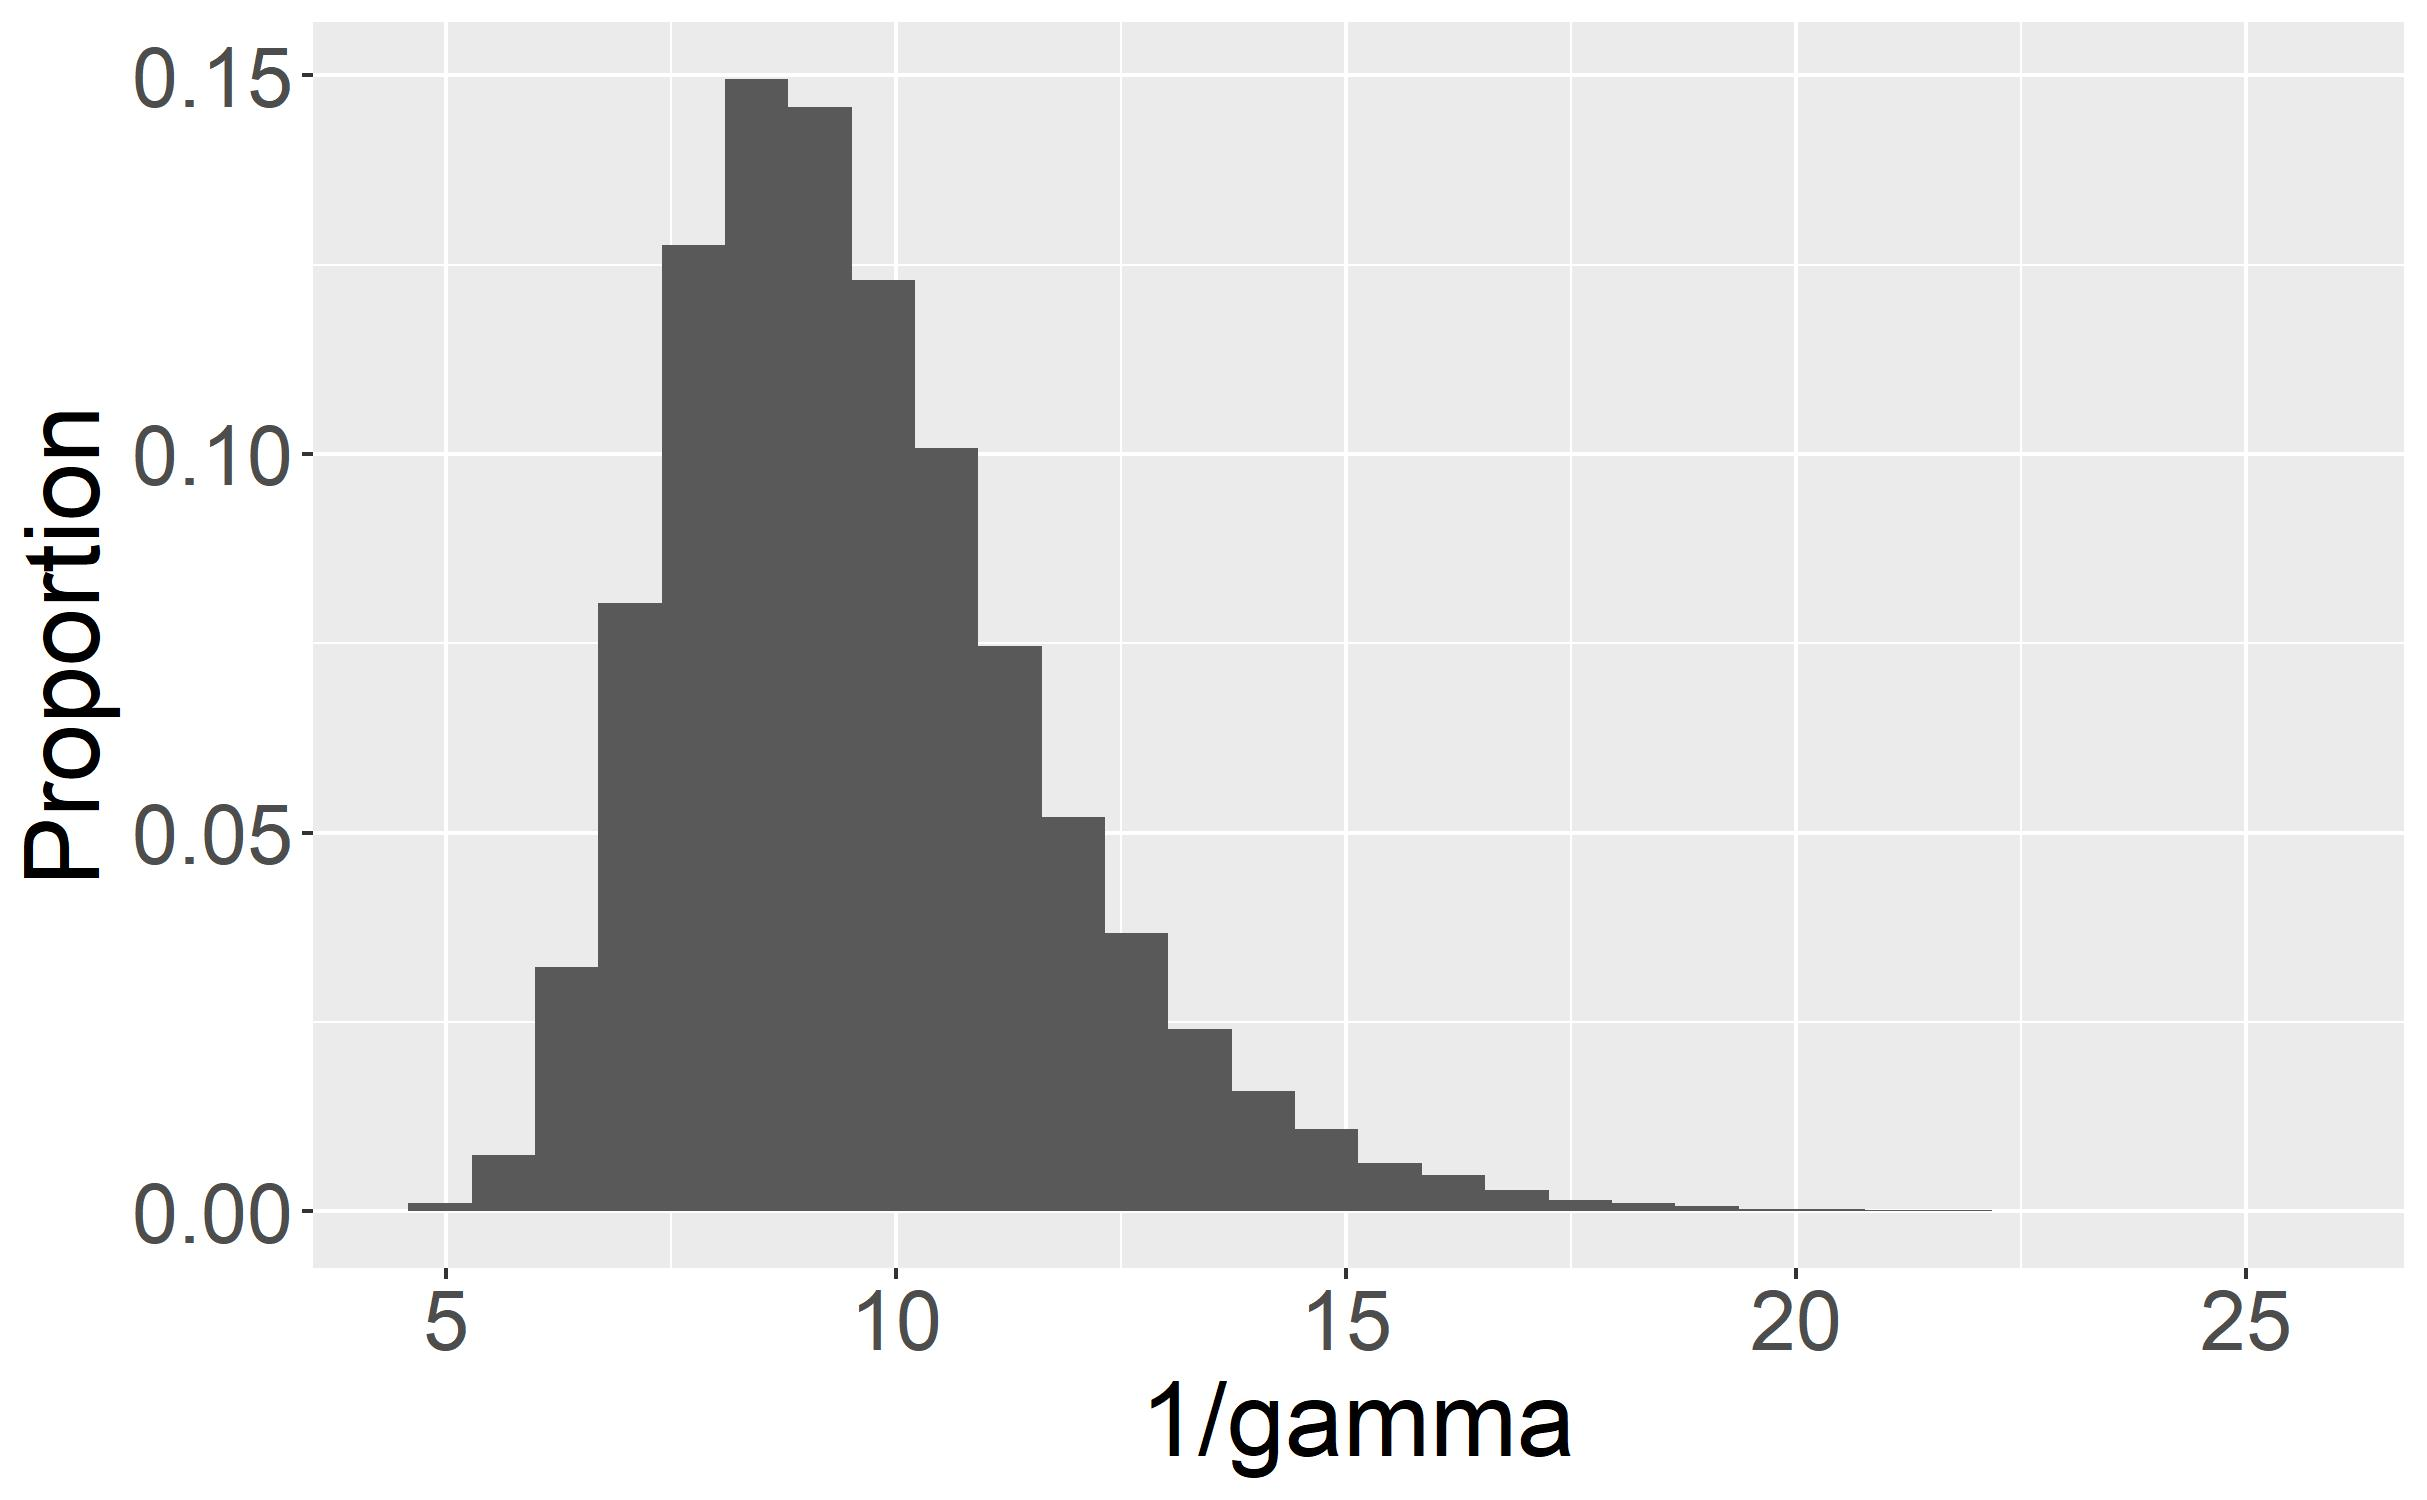
\includegraphics[width=\textwidth]{E5_expected_infection_length_hist}
			\caption{Posterior distribution}
			\label{fig:E5_gamma_hist}
		\end{subfigure}
		\hfill
		\begin{subfigure}[b]{0.45\textwidth}
			\centering
			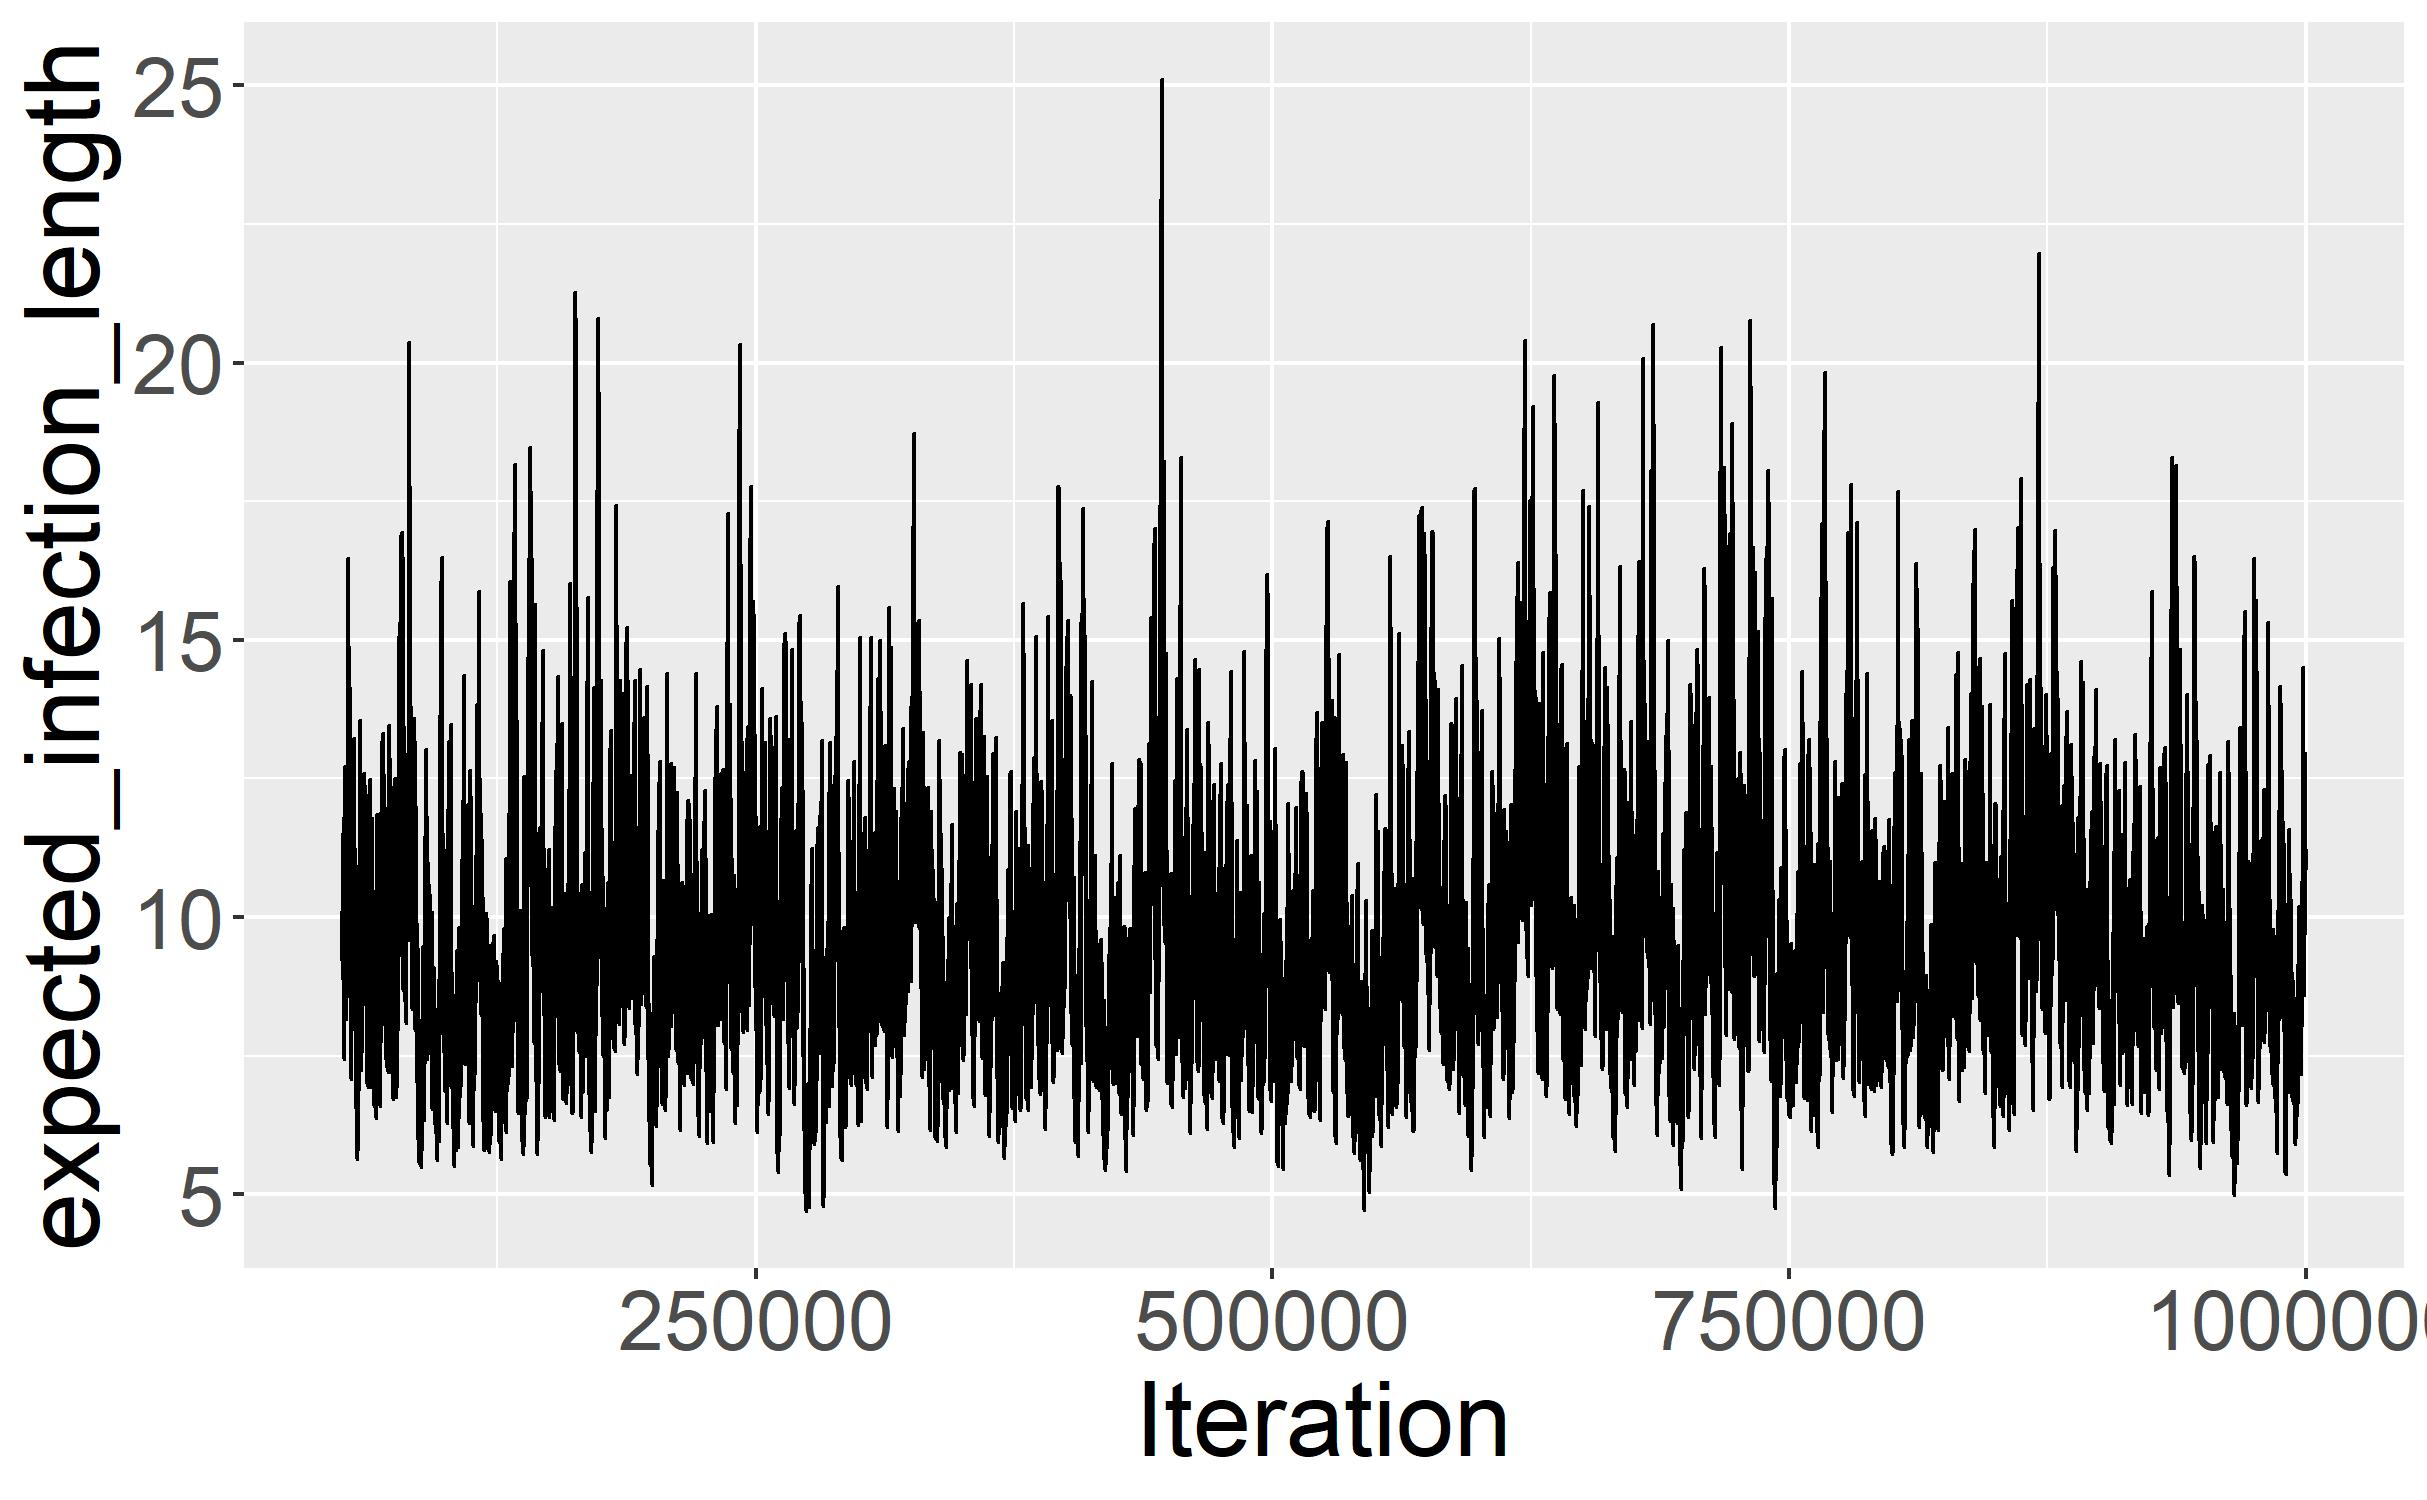
\includegraphics[width=\textwidth]{E5_expected_infection_length_tp}
			\caption{Traceplot}
			\label{fig:density_R0}
		\end{subfigure}
		\caption{Posterior distribution and traceplot of the expected infection length ($\gamma^{-1}$) for the Gu\'eck\'edou prefecture.}
		\label{fig:ebola}
	\end{figure}
	
	\section{Discussion and Conclusion}
	\label{sec:dis}
	The proposed method enables the classical Metropolis-Hastings algorithm to be an efficient way to conduct exact posterior inference under the stochastic SIR model, given only incidence data for infections. Existing attempts using Markov chain Monte Carlo either mix poorly or do not scale to populations of more than a few hundred individuals, while methods relying on forward simulation are limited to moderate-sized outbreaks and may suffer from degeneracy issues on a case-by-case basis depending on the amount of missing data. %Moreover, the simplifying assumptions in \cite{Fintzi.2020} or the approximate-Bayesian-computation framework of \cite{McKinley.2018}, which compromise targeting the exact posterior for computational reasons, generate biased estimates that may lead to spurious conclusions. 
	In contrast to methods that rely on approximate computation of simplifying assumptions necessitated by computational considerations \cite{McKinley.2018,Fintzi.2020}, 
	our data-augmented algorithm enables fast and exact Bayesian inference, even for large outbreaks, and leverages a well-studied, transparent MCMC framework with  guarantees of uniform ergodicity. %Most existing inferential methods for epidemic stochastic models are only applicable to prevalence data. To our knowledge, our algorithm is the first that permits exact Bayesian inference given incidence data.
	
	Central to the success of the DA-MCMC algorithm is an efficient proposal scheme for the latent variables that swiftly explores the latent space of epidemic paths that are compatible with the observed data. The PD-SIR process possesses three features that make it such an efficient proposal in our DA-MCMC. First, generating a PD-SIR process is extremely fast; it only requires the simulation of truncated exponential distributions, which can efficiently be realized via the inverse cumulative distribution function method. Moreover, the piece-wise constant infection rate of the PD-SIR is only updated $K$ times, as opposed to after each event in the SIR model. Second, generating a PD-SIR process that is constrained to be compatible with the observed incidence data can be done at no additional cost; in contrast, generating a SIR process compatible with the observed data would be prohibitively slow \cite{Hobolth.2009}. Third, the dynamics of the PD-SIR process closely resemble those of the SIR process: the removal dynamics are identical and, for short observation time intervals, the infection dynamics are also very similar in the two processes. The last feature 
	
	The first two features make the algorithm extremely fast. While existing data-augmented MCMC algorithms have only be applied to populations of a few hundred of individuals, the analysis of the Ebola outbreak in Gu\'eck\'edou shows that our algorithm can be applied to populations of up to 300,000 individuals in a reasonable amount of time.	
	The latter feature of the PD-SIR process enables the algorithm to update a large portion of the augmented data in each iteration while maintaining a healthy acceptance rate. As a result, the Markov chain makes large jumps in the latent space and has very good mixing properties. In contrast, existing DA-MCMC algorithms keep most of the latent space fixed across iterations \cite{Gibson.1998, ONeill.1999, Fintzi.2017} and their Markov chains therefore mix much more slowly.
	
	If the acceptance rate in the Metropolis-Hastings step for the latent data is too low, which can happen in large populations, our algorithm possesses a tuning parameter $\rho$ that determines the proportion of individuals whose trajectory is updated per iteration. Larger values for $\rho$ enable the chain to make larger steps in the latent space but may result in an excessively low acceptance rate, while smaller values of $\rho$ result in a higher acceptance rate but constrain the chain to make small jumps. Depending on the size of the population, different values of the tuning parameter are optimal. To find a value that optimizes the mixing properties of the chain, one can use several short runs of the algorithm with different values for $\rho$ and select the value that yields the largest effective size per second.
	
	%Exploring the latent space has been the bottleneck of DA-MCMC for stochastic epidemic models. The proposed method allows for efficient exploration of this space.
	
	The DA-MCMC algorithm proposed in this article is specific to 
	The stochastic SIR model, for which our algorithm is designed, is arguably a simplistic representation of the spread of disease. The model relies on assumptions such as perfect reporting, exponentially-distributed infectious periods, homogeneously mixing population and a constant infection rate. Our algorithm can be extended to models of increasing realism where these assumptions are relaxed. In future work, we will present applications to epidemic models with under-reporting \cite{Fintzi.2017}, non-Markovian dynamics \cite{Streftaris.2002}, non-homogeneous mixing \cite{Severo.1969} as well as time-varying infection rate \cite{Kypraios.2018}.
	
	\appendix
	
	\section{Proof of Theorem \ref{theo:ldp}}
	\label{app:ldp}
	
	Theorem \ref{theo:ldp} was first proved by \cite{Neuts.1971}. Ross \cite{Ross.1996} provides a simpler proof which we now give.
	
	\begin{proof}
	Consider a linear pure death process with $n$ particles and individual death rate $\mu$.
	Let $T_i$ be the time of the $i$th death. Then $W_1 = T_1 \sim \Exp(n\mu)$ and $W_i = T_i - T_{i-1} \sim \Exp((n-i)\mu)$ independently. Let $N$ be the number of deaths by time $t$. Then, 
	\begin{align*}
		& f(T_1 = t_1, \dots, T_N = t_N | N) \\
		& \propto f(T_1 = t_1, \dots, T_N = t_N, T_{N+1} > t) 1\{t_N < t\}\\
		& \propto f(W_1 = t_1, W_2 = t_2 - t_1, \dots, W_N = t_N - t_{N-1}, W_{N+1} > t - t_N) 1\{t_N < t\}\\
		& \propto \exp\{-n\mu t_1\} \exp\{-(n-1)\mu(t_2-t_1)\}\dots \exp\{-(n-N)\mu(t - t_N)\} 1\{t_N < t\}\\
		& \propto \exp\{-\mu t_1\}\exp\{-\mu t_2\} \dots \exp\{-\mu t_N\} 1\{t_N < t\}
	\end{align*}
	which corresponds to the kernels of independent exponential distribution truncated above by $t$. By the memoryless property of the exponential distribution, this results can be extended from the interval $(0, t]$ to any interval.
	
	\end{proof}
	
	\section{Proof of Proposition \ref{pro:uni}}
	\label{app:uni}
	
	We first present two lemmas that will be useful in the proof of Proposition \ref{pro:uni}.
	% Gamma 1
	\begin{lemma}
		\label{pro:ga1}
		Let $Ga(x;a,b) = \dfrac{a^b}{\Gamma(a)}x^{a-1}\exp\{-ab\}$ denote the density of the gamma distribution with shape $a$ and rate $b$ evaluated at $x$. Then
		\begin{equation}
			\label{eq:ga1}
			\inf_{0\le \beta\le B} Ga(x;a,b+\beta) = 
			\begin{cases}
				Ga(x;a,b), & x<x_a^* \\ Ga(x;a,b+B), & x\ge x_a^*
			\end{cases}
		\end{equation}	
		where $x_a^*=\frac{a}{B}\log\left( 1+\frac{B}{b}\right) $. Moreover,
		\begin{equation}
			\label{eq:ga2}
			\inf_{0\le \alpha\le A} Ga(x;a+\alpha,b) = 
			\begin{cases}
				Ga(x;a,b), & x>x_b^* \\ Ga(x;a+A,b), & x\le x_b^*
			\end{cases}
		\end{equation}
		where $x_b^*=\frac{1}{b}\left[ \frac{\Gamma(a+A)}{\Gamma(a)}\right]^{1/A}$. 
	\end{lemma}
	\begin{proof}
		Equation \eqref{eq:ga1} is proven in \cite{Jones.2004}. For Equation \eqref{eq:ga2}, note that $x_b^*$ is the only positive solution to $Ga(x;a,b) = Ga(x;a+A,b)$. Now, for all $0<x\le x_b^*$ and all $0\le\alpha\le A$, we have
		\begin{align*}
			\frac{Ga(x;a+A,b)}{Ga(x;a+\alpha,b)}
			& = b^{A-\alpha}x^{A-\alpha} \frac{\Gamma(a+\alpha)}{\Gamma(a+A)} \\
			& \le b^{A-\alpha}\left(\frac{1}{b}\left[ \frac{\Gamma(a+A)}{\Gamma(a)}\right]^{1/A} \right)^{A-\alpha} \frac{\Gamma(a+\alpha)}{\Gamma(a+A)} \\
			& = \left[ \frac{\Gamma(a+A)}{\Gamma(a)}\right]^{(A-\alpha)/A} \frac{\Gamma(a+\alpha)}{\Gamma(a+A)} \\
			& = \left[
			\frac{\left(\frac{\Gamma(a+A)}{\Gamma(a)}\right)^{1/A}}{\left(\frac{\Gamma(a+A)}{\Gamma(a+\alpha)}\right)^{1/(A-\alpha)}}
			\right]^{A-\alpha} \\
			& = \left( \frac{\Gamma_{a,a+A}}{\Gamma_{a+\alpha, a+A}}\right)^{A-\alpha} \\
			& \le 1,
		\end{align*}
		where $\Gamma_{d,e} = \left( \frac{\Gamma(e)}{\Gamma(d)} \right)^{\frac{1}{e-d}}$ is a geometric mean,
		and where the last inequality holds because $\Gamma_{a,a+A}\le\Gamma_{a+\alpha, a+A}$.
		The case $x>x_b^*$ is analogous and is omitted for brevity.
	\end{proof}
	
	Figures \ref{fig:gam1a} and \ref{fig:gam1b} illustrate these two results. Lemma \ref{pro:ga1} can be used to obtain a closed form solution to the minimization of a gamma density of the form
	\begin{equation}
		\label{eq:ga}
		Ga(x;a+\alpha,b+\beta) = \frac{(b+\beta)^{a+\alpha}}{\Gamma(a+\alpha)}x^{a+\alpha-1}\exp\{-x(b+\beta)\}, \quad 0\le\alpha\le A, 0\le\beta\le B.
	\end{equation}
	jointly over $\alpha$ and $\beta$ for each value of $x$. To this end, we establish the following technical lemma.
	% Gamma 2 (joint)
	\begin{lemma}	
		\label{pro:ga2}
		For a fix $x>0$, the density $Ga(x;a+\alpha,b+\beta)$ is minimized by $(\alpha, \beta) \in \{(A, 0), (0, B)\}$, the minimizing set of values depending on $x$. In particular,	
		$$\inf_{\begin{aligned}
				0\le \alpha\le A \\ 0\le \beta\le B
		\end{aligned}}Ga(x;a+\alpha,b+\beta) = 
		\begin{cases}
			Ga(x;a+A,b)                     , & x<x_a         \text{ or } x<x_{a+A}^* \vee x_b^*\\
			Ga(x;a,b+B)                     , & x_{a+A}^* < x \text{ or } x_a^* \wedge x_{b+B}^* < x\\
			\min\{Ga(x;a+A,b), Ga(x;a,b+B)\}, & x_a^* \wedge x_b^*\le x < x_{a+A}^* \vee x_{b+B}^*\\
		\end{cases}$$
	\end{lemma}
	
		\begin{proof}
		Given $x>0$, \eqref{eq:ga1} shows that for a fixed $\alpha$, the gamma density \eqref{eq:ga} is minimized by $\beta \in \{0, B\}$. Similarly,  \eqref{eq:ga2} shows that for a fixed $\beta$, $\alpha \in \{0, A\}$ minimizes \eqref{eq:ga}. This implies that for a fixed $x>0$, the gamma density \eqref{eq:ga} is minimized by $(\alpha, \beta) \in \{(0,0), (A, 0), (0, B), (A,B)\}$.
		
		A case-by-case analysis of the nine possibilities
		$$(x<x_a^*; x_a^*<x<x_{a+A}^*; x_{a+A}^* < x )\times(x<x_{b+B}^*; x_{b+B}^*<x<x_b^*; x_b^* < x)$$
		is presented in Table \ref{tab:ga9} and shows that it is sufficient to consider $(\alpha, \beta) \in \{(A, 0), (0, B)\}$.
		
		\begin{table}[H]
			\centering
			\begin{tabular}{l|c c c}
				& $x<x_a^*$  & $x_a^*\le x<x_{a+A}^*$ & $x_{a+A}^* < x$ \\
				\hline
				$x<x_b^*$              & $(a+A, b)$ & $(a+A, b)$             &                 \\
				$x_b^*\le x<x_{b+B}^*$ & $(a+A, b)$ &  ad hoc                & $(a, b+B)$      \\
				$x_{b+B}^* < x$        &            & $(a, b+B)$             & $(a, b+B)$ \\
				\hline
			\end{tabular}
			\caption{Values of $(\alpha, \beta)$ that minimize $Ga(x;a+\alpha,b+\beta)$ for different values $x$.}
			\label{tab:ga9}
		\end{table}
		
		The two empty entries in Table \ref{tab:ga9} correspond to configurations that are impossible. Indeed, we must have $x_b^* > x_a^*$ and $x_{a+A}^* > x_{b+B}^*$ for all $a, A, b, B$ since
		$$
		\frac{x_b^*}{x_a^*} = \dfrac{\left(\frac{\Gamma(a+A)}{\Gamma(a)}\right)^{1/A} b^{-1} }{a B^{-1} \log\left( 1+B/b\right)} = \dfrac{\left(\frac{\Gamma(a+A)}{\Gamma(a)}\right)^{1/A}}{a} \dfrac{B/b}{\log\left( 1+B/b\right)} = \dfrac{\Gamma_{a,a+A}}{a} \dfrac{B/b}{\log\left( 1+B/b\right)} \ge 1
		$$
		where the inequality hold since $a \le \Gamma_{a,a+A}$ and $\dfrac{y}{\log\left( 1+y\right)}\ge1$,
		and
		$$
		\frac{x_{b+B}^*}{x_{a+A}^*} = \dfrac{\left(\frac{\Gamma(a+A)}{\Gamma(a)}\right)^{1/A} (b+B)^{-1} }{(a+A) B^{-1} \log\left( 1+B/b\right)} = \dfrac{\Gamma_{a,a+A}}{a+A} \dfrac{B}{b+B} \dfrac{1}{\log\left( 1+B/b\right)} \le 1
		$$
		where the inequality holds since $\Gamma_{a,a+A} \le a+A$.
		
		If $x_a^* \wedge x_{b+B}^*\le x < x_{a+A}^* \vee x_{b}^*$, which corresponds to the middle entry of the center column in Table \ref{tab:ga9}, then one needs to directly check which set of values in $\{(0,0), (A, 0), (0, B), (A,B)\}$ minimizes \eqref{eq:ga}. In fact, it is sufficient to consider only $\{(A,0), (0, B)\}$ since
		$$Ga(x, a+A, b) \le \begin{cases}
			Ga(x;a,b), & x < x_b^* \\
			Ga(x;a+A,b+B), & x < x_{a+A}^* 
		\end{cases}$$
		and
		$$Ga(x, a, b+B) \le \begin{cases}
			Ga(x;a,b), & x > x_a^* \\
			Ga(x;a+A,b+B), & x > x_{b+B}^* 
		\end{cases}$$
	\end{proof}
	
	
	\begin{figure}	

	\end{figure}
	
	\begin{figure}
		\centering
		\begin{subfigure}[b]{0.32\textwidth}
			\centering
			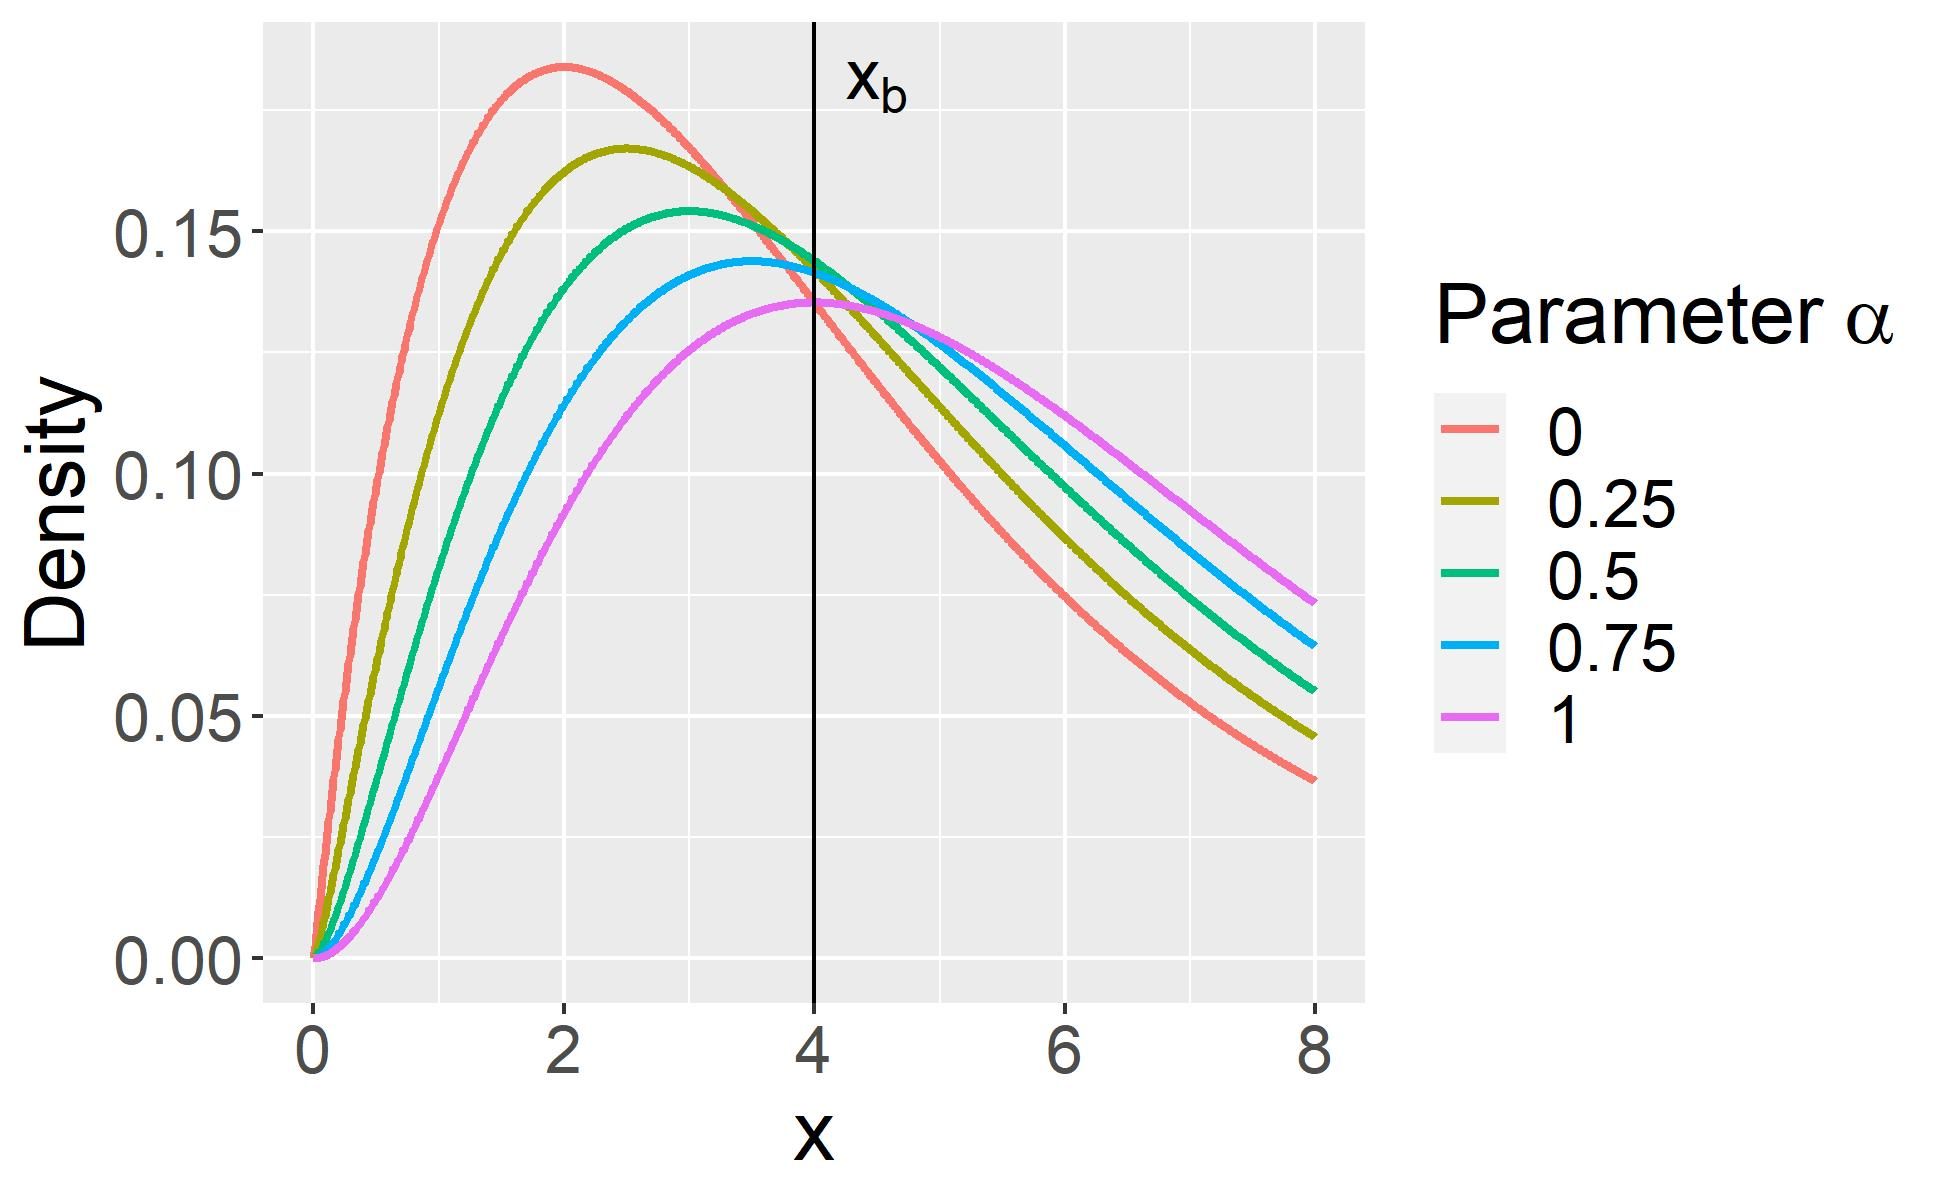
\includegraphics[width=\textwidth]{gamma1a.jpg}
			\caption{$\alpha \in [0, 1]$, $\beta=0$}
			\label{fig:gam1a}
		\end{subfigure}
		\hfill
		\begin{subfigure}[b]{0.32\textwidth}
			\centering
			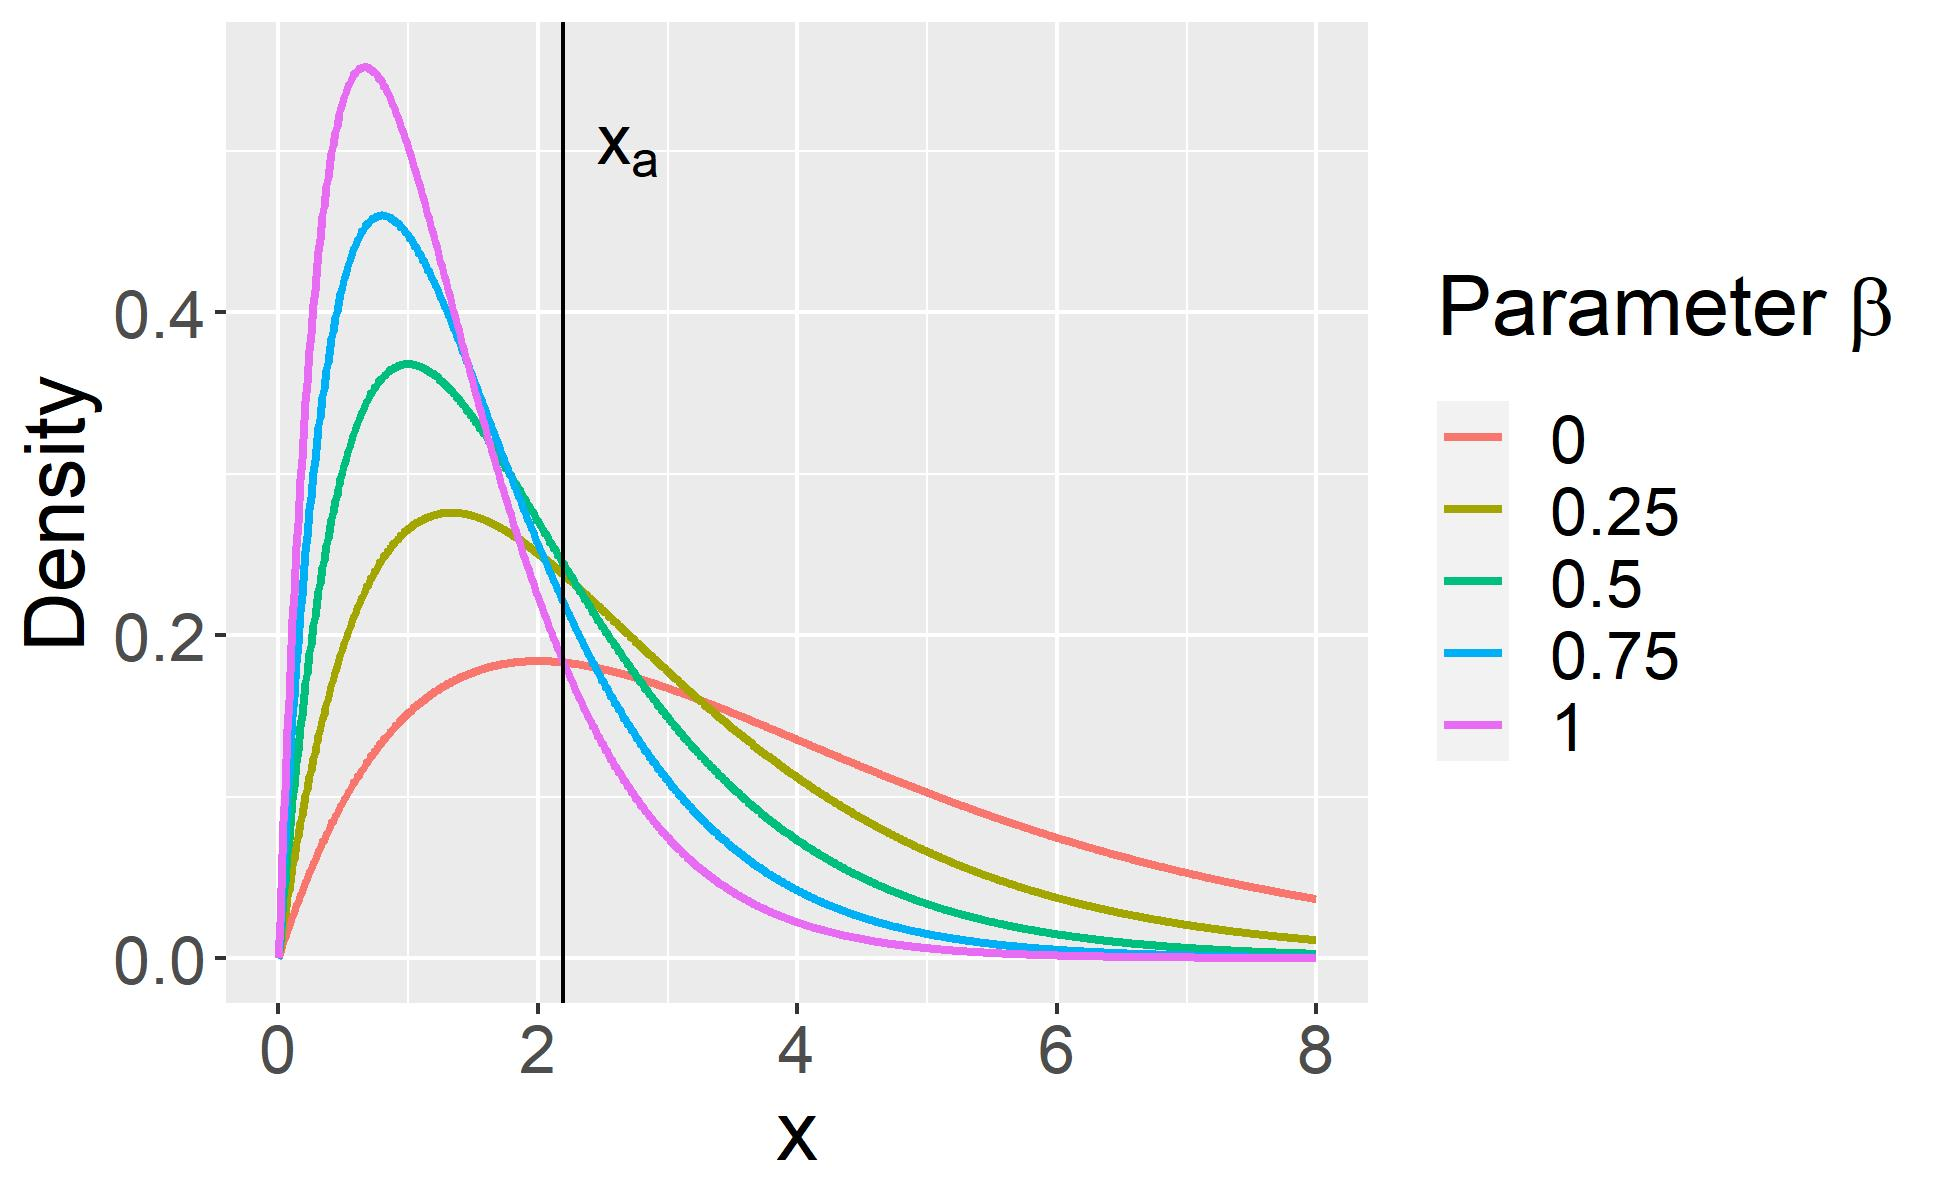
\includegraphics[width=\textwidth]{gamma1b.jpg}
			\caption{$\alpha = 0$, $\beta \in [0, 1]$}
			\label{fig:gam1b}
		\end{subfigure}
		\hfill
		\begin{subfigure}[b]{0.32\textwidth}
		    \centering
		    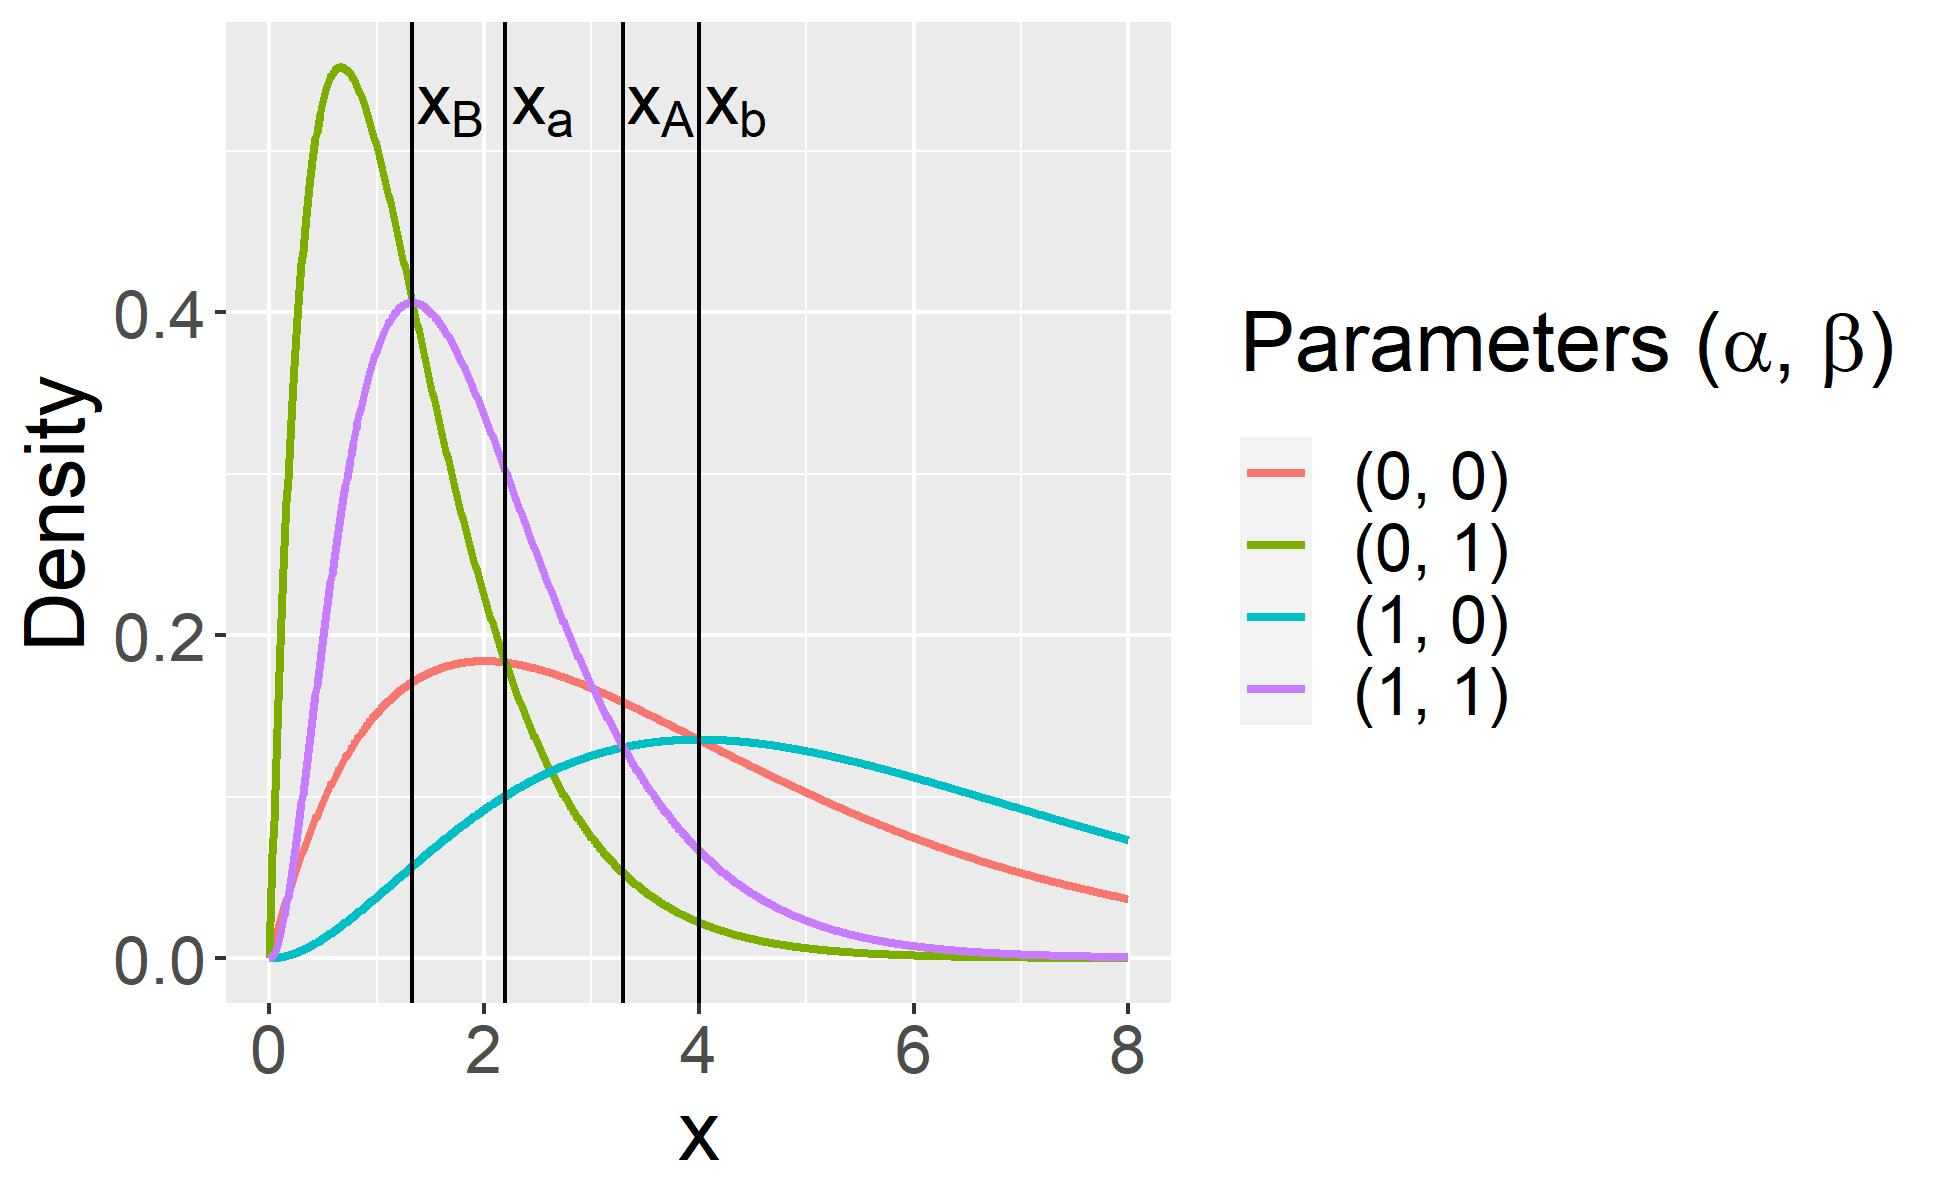
\includegraphics[width=\textwidth]{gamma2.jpg}
			\caption{$\alpha \in \{0,1\}$, $\beta \in \{0,1\}$}
		\label{fig:gam2}
		\end{subfigure}
		\caption{Example of minorization of the density of a gamma distribution $Ga(2+\alpha, 0.5+\beta)$.}
		\label{fig:gam}
	\end{figure}
	
	%\noindent
	We can now proceed with the proof of Proposition \ref{pro:uni}.
	
	\begin{proof}
		The transition kernel $P = P_{\theta} P_{\z}$ is a composition of two kernels. The kernel $P_{\theta}$ updates the parameters $\theta$ while keeping the latent data $\z$ fixed, and $P_{\z}$ update $\z$ while keeping $\theta$ fixed. %A one-step transition therefore corresponds to the following scheme 
		%$$\x_1 = (\theta_1, \z_1) \rightarrow (\theta_2, \z_1) \rightarrow (\theta_2, \z_2) = \x_2.$$
		We therefore have
		$$P((\theta_1, \z_1), (d\theta_2, d\z_2)) = P_\theta(\theta_1, d\theta_2 | \z_1) P_\z(\z_1, d\z_2 | \theta_2)$$
		where
		\begin{align}
		\label{eq:Pth}
		    P_\theta(\theta_1, d\theta_2 | \z_1)
		    & = \pi(d\theta_2 | \z_1) \\
		    & = \pi(\beta_2 | \z_1) \pi(\gamma_2 | \z_1) d\beta_2 d\gamma_2 \nonumber
		\end{align}
		corresponds to the transition kernel of a Gibbs sampler and
		\begin{align}
		\label{eq:Pz}
		    P_\z(\z_1, d\z_2 | \theta_2)
		    & = Q(d\z_2 | \theta_2) \alpha((\theta_2, \z_1),(\theta_2, \z_2)) + \delta_{\z_1}(d\z_2)\int(1-\alpha((\theta_2, \z_1),(\theta_2, \z_2))) Q(d\z_2| \theta_2) \nonumber \\
			& \ge Q(d\z_2| \theta_2) \alpha((\theta_2, \z_1),(\theta_2, \z_2)) \\
			& = q(\z_2| \theta_2) \min\left\lbrace 1, \dfrac{\pi(\theta_2, \z_2)q(\z_1| \theta_2)}{\pi(\theta_2, \z_1)q(\z_2| \theta_2)} \right\rbrace d\z_2 \nonumber
		\end{align}
		corresponds to a Metropolis-Hasting transition kernel in which a new configuration of the latent data is generated from the proposal kernel $Q$ conditionally on the current value of the parameters $\theta_2$, but independently of the current configuration $\z_1$. The density $q$ of the proposal kernel $Q$ is given in \eqref{eq:q}.
		
		To show that $\chi$ is a small state, it suffices to show that there exists a positive function $k$ such that
		\begin{equation}
		    \label{eq:min}
		    k(\theta_2, \z_2) \le \pi(\beta_2 | \z_1) \pi(\gamma_2 | \z_1) q(\z_2; \theta_2) \min\left\lbrace 1, \dfrac{\pi(\theta_2, \z_2)q(\z_1| \theta_2)}{\pi(\theta_2, \z_1)q(\z_2|\theta_2)} \right\rbrace
		\end{equation}
		for all $\theta_1 \in \chi_\theta$ and all $\z_1 \in \chi_\z.$
		Indeed, suppose that we can find a positive function $k$ satisfying the inequality \eqref{eq:min}, then for any set $A$ and any $(\theta, \z)$ we have, by \eqref{eq:Pth}, \eqref{eq:Pz} and \eqref{eq:min},
		\begin{align*}
		    P((\theta, \z), A)
		    & \ge \int_A \pi(\theta' | \z) \pi(\beta' | \z) \pi(\gamma' | \z) \min\left\lbrace 1, \dfrac{\pi(\theta', \z')q(\z| \theta')}{\pi(\theta', \z)q(\z'|\theta')} \right\rbrace d(\beta', \gamma', \z') \\
		    & \ge \int_A k(\theta', \z') d(\theta', \z') \\
		    & = \epsilon \nu(A)
		\end{align*}
		with $\epsilon = \int k(\theta, \z) d(\theta, \z)$ a positive constant and $\nu(A) = \epsilon^{-1} \int_A k(\theta, \z) d(\theta, \z)$ a probability measure. 
		
		We now construct a positive function $k$ satisfying \eqref{eq:min}. The inequality depends on $(\theta_1, \z_1)$ only through the full conditional distributions $\pi(\beta_2 | \z_1)$ and $\pi(\gamma_2 | \z_1)$ and the ratio $\dfrac{q(\z_1| \theta_2)}{\pi(\theta_2, \z_1)}$.
		It therefore suffices to find positive functions $k_\beta, k_\gamma$ and $k_r$ such that, for all $\z_1$,
		$$k_\beta(\beta_2) \le \pi(\beta_2 | \z_1),
		\quad k_\gamma(\gamma_2) \le \pi(\gamma_2 | \z_1),
		\quad \text{and} \quad k_r(\theta_2) \le \dfrac{q(\z_1|\theta_2)}{\pi(\theta_2, \z_1)}.$$
		
		First, we can obtain a closed form minorization of $\pi(\beta_2| \z_1)$ using Proposition \ref{pro:ga1} as follows,
		\begin{align*}
			\pi(\beta_2| \z_1) 
			& = Ga\left(\beta_2; a_{\beta} + n_I, b_{\beta} + \int_{0}^{t_{end}}S(t)I(t)dt\right) \\
			& \ge \inf_{\begin{aligned}
				 0\le \int_{0}^{t_{end}} S(t)I(t)dt \le n(n_I+I_0) t_{end}
		\end{aligned}}   Ga\left(\beta_2; a_{\beta} + n_I, b_{\beta} + \int_{0}^{t_{end}}S(t)I(t)dt\right) \\
			& = \min\{Ga(\beta_2;a_{\beta}+n_I, b_{\beta}), Ga(\beta_2;a_{\beta}+n_I,b_{\beta}+n(n_I+I_0) t_{end})\} \\
			& = k_\beta(\beta_2) > 0
		\end{align*}
		since $n_I = \sum_k I_k$ is known and the sufficient statistic from $\z_1$, 
		$\int_{0}^{t_{end}}S(t)I(t)dt$, is bounded between $0$ and $n (n_I+I_0)t_{end}$. Similarly, by Proposition \ref{pro:ga2}, we can minorize $\pi(\gamma_2| \z_1)$ as follows,
		\begin{align*}
			\pi(\gamma_2| \z_1) 
			& = Ga\left(\gamma_2; a_{\beta} + n_R, b_{\beta} + \int_{0}^{t_{end}}I(t)dt\right)  \\
			& \ge \inf_{\begin{aligned}
				 0 \le n_R &\le n_I + I_0, \\
				 0 \le \int_{0}^{t_{end}} I(t)dt &\le (n_I+I_0) t_{end}
		\end{aligned}} Ga\left(\gamma_2; a_{\beta} + n_R, b_{\beta} + \int_{0}^{t_{end}}I(t)dt\right) \\
			& = \min\{		Ga(\gamma_2;a_{\gamma}+n_R+I_0,b_{\gamma}), Ga(\gamma_2;a_{\gamma},b_{\gamma}+(n_I+I_0) t_{end})\} \\
			& = k_\gamma(\gamma_2) > 0
		\end{align*}
		since the sufficient statistics from $\z_1$, $n_R$ and $\int_{0}^{t_{end}}I(t)dt$, are respectively bounded between $0$ and $n_I + I_0$, and between $0$ and $(n_T+I_0) t_{end}$.
		
		Finally, the ratio $\dfrac{q(\z_1|\theta_2)}{\pi(\theta_2, \z_1)}$ can be minorized as follows, %\ram{(in the second inequality, minimize the whole numerator in terms of $I(.)$ instead of its each factors (=> use previous proof minimizing the proposal density); this will provide a better bound)}
		\begin{align*}
		    \dfrac{q(\z_1|\theta_2)}{\pi(\theta_2, \z_1)} 
		    & = \dfrac{\prod_{k=1}^K \prod_{j\in \mathcal{I}_k} \TruncExp(z^I_j; \mu_k, t_{k-1}, t_k) \prod_{i=1}^n (1-p_i)^{\mathbf{1}\{z^R_i=\infty\}} \left(p_i \TruncExp(z^R_i;\gamma, z^I_i, t_{end})\right)^{\mathbf{1}\{z^R_i \le t_{end}\}}}
        	{\beta^{n_I} \prod_{l\in \mathcal{I}} I(z^I_l) \gamma^{n_R} \exp\{-\beta \int_0^{t_{end}} S(t)I(t)dt -\gamma \int_0^{t_{end}} I(t)dt\}} \\
        	& = \dfrac{\prod_{k=1}^K \prod_{j\in \mathcal{I}_k} \TruncExp(z^I_j; \mu_k, t_{k-1}, t_k)}
        	{\prod_{l\in \mathcal{I}} \beta I(z^I_l) \exp\{-\beta \int_0^{t_{end}} S(t)I(t)dt\}}\\
        	& = \dfrac{\prod_{k=1}^K \prod_{j\in \mathcal{I}_k} \dfrac{\beta I(t_{k-1}) \exp\{-\beta I(t_{k-1}) (z^I_j - t_{k-1})\}}{1-\exp\{-\beta I(t_{k-1})(t_k - t_{k-1})\}}}
        	{\prod_{l\in \mathcal{I}} \beta I(z^I_l) \exp\{-\beta \int_0^{t_{end}} S(t)I(t)dt\}}\\
        	%& = \dfrac{\prod_{k=1}^K \prod_{j\in \mathcal{I}_k} \dfrac{I(t_{k-1}) \exp\{-\beta I(t_{k-1}) (z^I_j - t_{k-1})\}}{1-\exp\{-\beta I(t_{k-1})(t_k - t_{k-1})\}}}
        	%{\prod_{l\in \mathcal{I}} I(z^I_l) \exp\{-\beta \int_0^{t_{end}} S(t)I(t)dt\}}\\
        	& \ge \dfrac{\prod_{k=1}^K \prod_{j\in \mathcal{I}_k} I(t_{k-1}) \exp\{-\beta I(t_{k-1}) (z^I_j - t_{k-1})\}}
        	{\prod_{l\in \mathcal{I}} I(z^I_l) \exp\{-\beta \int_0^{t_{end}} S(t)I(t)dt\}}\\
        	& \ge \dfrac{\prod_{k=1}^K \prod_{j\in \mathcal{I}_k} \exp\{-\beta n (t_k - t_{k-1})\}}
        	{n^{n_I}}\\
        	& = k_r(\beta_2),
		\end{align*}
		where the second equality holds since the contribution of the removal times in the numerator and the denominator cancel each other as the removal times are generated from the same distribution under the SIR and the PD-SIR processes:
        \begin{align*}
        	& \dfrac{\prod_{i=1}^n (1-p_i)^{\mathbf{1}\{z^R_i=\infty\}} (p_i \TruncExp(z^R_i;\gamma, z^I_i, t_{end}))^{\mathbf{1}\{z^R_i \le t_{end}\}}}{\gamma^{n_R} \exp\{- \gamma \int_0^{t_end} I(t)dt\}} \\
        	& = \dfrac{\prod_{j \in \mathcal{R}^c} \exp\{-\gamma(t_{end}-z^I_j)\} \prod_{k \in \mathcal{R}} (1-\exp\{\gamma(t_{end}-z^I_k)\}) \dfrac{\gamma \exp\{-\gamma (z^R_k - z^I_k)\}}{1-\exp\{\gamma(t_{end}-z^I_k)\}} }{\gamma^{n_R} \exp\{ \gamma \sum_{i=1}^n \min\{z^R_i, t_{end}\} - z^I_i\}} \\
        	& = \dfrac{\exp\{-\gamma \sum_{j \in \mathcal{R}^c}(t_{end}-z^I_j)\} \gamma^{n_R} \exp\{-\gamma \sum_{k\in R}(z^R_k - z^I_k)\} }{\gamma^{n_R} \exp\{-\gamma[\sum_{j \in \mathcal{R}^c}(t_{end}-z^I_j) + \sum_{k\in \mathcal{R}}(z^R_k - z^I_k)] \}} \\
        	& = 1,
        \end{align*}
        the first inequality holds because $1-\exp\{-\beta I(t_{k-1})(t_k - t_{k-1})\} \le 1$ and the second inequality holds because $1\le I(.) \le n$,  $0\le\int_0^{t_{end}} S(t)I(t)dt$ and $z^I_j \le t_k$ when $j\in\mathcal{I}_k$.
		
		Taken together, these inequalities give
		\begin{align*}
		\pi(\beta_2 | \z_1) \pi(\gamma_2 | \z_1) q(\z_2; \theta_2) \min\left\lbrace 1, \dfrac{\pi(\theta_2, \z_2)q(\z_1| \theta_2)}{\pi(\theta_2, \z_1)q(\z_2
		|\theta_2)} \right\rbrace
		& \ge k_\beta(\beta_2) k_\gamma(\gamma_2) q(\z_2; \theta_2) \min\left\lbrace 1, k_r(\beta_2) \dfrac{\pi(\theta_2, \z_2)}{q(\z_2|\theta_2)} \right\rbrace \\
		& = k(\theta_2, \z_2)
		\end{align*}
		for all $\theta_1 \in \chi_\theta$ and all $\z_1 \in \chi_\z$, which completes the proof.

	\end{proof}
	
	% Gamma 2
	%can be used to minorize a density of the form
	% \begin{equation}
	% 	\label{eq:ga}
	% 	Ga(x;a+\alpha,b+\beta) = \frac{(b+\beta)^{a+\alpha}}{\Gamma(a+\alpha)}x^{a+A-1}\exp\{-x(b+B)\}, \quad 0\le\alpha\le A, 0\le\beta\le B.
	% \end{equation}
	% over $\alpha$ and $\beta$ for each value of $x$. We can show the following.
	% \begin{lemma}	
	% 	\label{pro:ga2}
	% 	For a fix $x>0$, the density $Ga(x;a+\alpha,b+\beta)$ is minimized by $(\alpha, \beta) \in \{(A, 0), (0, B)\}$, the minimizing set of values depending on $x$. In particular,	
	% 	$$\inf_{\begin{aligned}
	% 			0\le \alpha\le A \\ 0\le \beta\le B
	% 	\end{aligned}}Ga(x;a+\alpha,b+\beta) = 
	% 	\begin{cases}
	% 		Ga(x;a+A,b)                     , & x<x_a         \text{ or } x<x_{a+A}^* \vee x_b^*\\
	% 		Ga(x;a,b+B)                     , & x_{a+A}^* < x \text{ or } x_a^* \wedge x_{b+B}^* < x\\
	% 		\min\{Ga(x;a+A,b), Ga(x;a,b+B)\}, & x_a^* \wedge x_b^*\le x < x_{a+A}^* \vee x_{b+B}^*\\
	% 	\end{cases}$$
	% \end{lemma}
	
%%%%%%%%%%%%%%%%%%%%%%%%%%%%%%%%%%%%%%%%%%%
	
	% Truncated Exponential
%	Proof of Lemma \ref{pro:tru}
	
%	\begin{proof}
%		Remember that $\TruncExp(u; \mu, 0, u) = \frac{\mu \exp\{-u\mu\}}{1-\exp\{-u\mu\}}$ is the density of an exponential distribution bounded above by $u$.
%		\begin{align*}
%			\frac{d}{d\mu}\TruncExp(u; \mu, 0, u)
%			& = \left(\frac{\exp\{-u\mu\}}{1-\exp\{-u\mu\}} \right) \left[ 1-\mu u - \mu u \left(\frac{\exp\{-u\mu\}}{1-\exp\{-u\mu\}} \right) \right]
%		\end{align*}
%		Now let $g(\mu) = 1-\mu u - \mu u \left(\frac{\exp\{-u\mu\}}{1-\exp\{-u\mu\}} \right)$. By L'H\^{o}pital's rule, $g(0) = 0$. Moreover, for $\mu>0$, we have
%		\begin{align*}
%			g'(\mu)
%			& = - \mu \left(1+\frac{\exp\{-u\mu\}}{1-\exp\{-u\mu\}} \right) \left[ 1-u\mu \left(\frac{\exp\{-u\mu\}}{1-\exp\{-u\mu\}} \right) \right]  \\
%			& = - \mu \left(1+\frac{\exp\{-u\mu\}}{1-\exp\{-u\mu\}} \right) \left[ 1- \frac{u\mu}{\exp\{u\mu\}-1} \right] \\
%			& \le 0
%		\end{align*}
%		where the inequality follows from $\frac{u\mu}{\exp\{u\mu\}-1}\le1$.
%		This implies that $g(\mu) \le 0$ for $\mu>0$. We therefore have $\frac{d}{d\mu}\TruncExp(u; \mu, 0, u) \le 0$ and the result of the proposition follows.
%	\end{proof}

	
	\bibliographystyle{plain}
	\bibliography{bibliography}
	
\end{document}